\chapter{Other cuts and corrections}
\label{other}

\section{Fiducial cuts}
\label{fiduc} The CLAS detector has an active detection solid angle
that is obviously smaller than $4\pi$. This is in part due to the space filled with
the torus field coils: the angles covered by the coils are not
equipped with any detection system and therefore form a "dead" area
for detection. Moreover, different studies and analyses have shown
that also the edges of the active area do not provide a safe region
for particle reconstruction, being affected by rescattering from the
coil, field distortions, and similar effects. Therefore it is now
common practice to accept for the analysis only events inside
specific fiducial cuts, i.e. cuts on the kinematic variables
(momentum and angles) of each particle. This method guarantees that the
reconstructed events accepted in the analysis include only particles
detected in "safe" areas of the detector, that is where the
acceptance is thought to be well understood. These cuts are applied for both real events and Monte Carlo reconstructed events and produce a
reduction factor in the number of events accepted in each kinematic
bin that is called detector acceptance.

\subsection{Fiducial cuts for negatively charged particles}
\label{fiduch_nagative}

In the CLAS experiments with the normal direction of the torus magnetic field, like in e1e experiment, negatively charged particles are inbending. For that type of particles sector independent, symmetrical, and momentum dependent cuts are applied. To establish the shape of these cuts relatively flat areas in $\varphi$ distributions are selected. For that purpose all events are binned in  the particle momentum and the particle polar angle $\theta$ (see Fig.~\ref{fig:fiduch_negative_1d}). In Fig.~\ref{fig:fiduch_negative_1d} $\varphi$ distributions are shown for one slice over momentum and for various bins in $\theta$ for electrons (left side plots) and $\pi^{-}$ (right side plots). Events between the vertical lines in Fig.~\ref{fig:fiduch_negative_1d} are selected for further analysis. The analytical shape of these cuts is given by Eq.~\ref{eq:fiduch_electrons} for electrons and Eq.~\ref{eq:fiduch_pim} for $\pi^{-}$
\begin{equation}
\begin{aligned}
& \theta_{min}  = 9.7 + 17/(P_{e'} + 0.2) \\
& \delta\varphi_{e'}  = p_{1}sin(p_{2}(\theta_{e'}-\theta_{min}))^{p_{3}+p_{4}/\theta_{e'}+p_{5}/\theta_{e'}^{2}} + p_{6}  \\
& p_{1}  = 37.3(0.85 + 1.1P_{e'}) \\
& p_{2}  = 0.01745 \\
& p_{3}  = p_{1}/37.3 \\
& p_{4}  = -62.8 - 30P_{e'} \\
& p_{5}  = 1525 \\
& p_{6}  = 0  \label{eq:fiduch_electrons}
\end{aligned}  
\end{equation}

\begin{equation}
\begin{aligned}
& \theta_{min} = 11 + 8/(0.472P_{\pi^{-}} + 0.117) \\
& \delta\varphi_{\pi^{-}} = p_{1}sin(p_{2}(\theta_{\pi^{-}}-\theta_{min}))^{p_{3}+p_{4}/\theta_{\pi^{-}}+p_{5}/\theta_{\pi^{-}}^{2}} + p_{6} \\
& p_{1} = 30.5 \\
& p_{2} = 0.01745 \\
& p_{3} = 0.705 + 1.1P_{\pi^{-}} \\
& p_{4} = -63.2 - 33.3P_{\pi^{-}} \\
& p_{5} = 1530 \\
& p_{6} = -1 \label{eq:fiduch_pim}
\end{aligned}  
\end{equation}
where $P_{e'}$ and $P_{\pi^{-}}$ are the momenta of the particles in GeV, $\theta_{e'}$ and $\theta_{\pi^{-}}$ are the polar angles of the particles in degrees. $\delta\varphi_{e'}$ and $\delta\varphi_{\pi^{-}}$ are the portions of the polar angle
$\varphi$ accepted by the fiducial cut, or in other words if
$\theta > \theta_{min}$ and $|\varphi| < \delta\varphi$ then the particle is accepted. 
The functions~\ref{eq:fiduch_electrons},\ref{eq:fiduch_pim} are shown in 2D plots $\varphi$ versus $\theta$ in Fig.~\ref{fig:eother_cuts_negative_fiduch_2d} for electrons (left side) and $\pi^{-}$ (right side).

There are some additional inefficient areas that are not related to the gaps between CLAS sectors. These areas are typicaly caused by drift chamber and time-of-flight system inefficiencies (dead wires or PMTs). Some of them are reproduced in Monte Carlo simulation, while others are not. To exclude the latter from the analysis additional fiducial cuts on $\theta$ versus momentum distributions are applied. These cuts are individual for each CLAS sector. They are shown by the black curves for real and Monte Carlo events in Fig.~\ref{fig:other_cuts_negaitive_th_vs_p_electronss} for electrons and in Fig.~\ref{fig:other_cuts_negaitive_th_vs_p_pions} for $\pi^{-}$. For the electron distributions in Fig.~\ref{fig:other_cuts_negaitive_th_vs_p_electronss} only CLAS sector five is shown since there are no dead areas in other sectors.


\begin{figure}[htp]
\begin{center}
\fbox{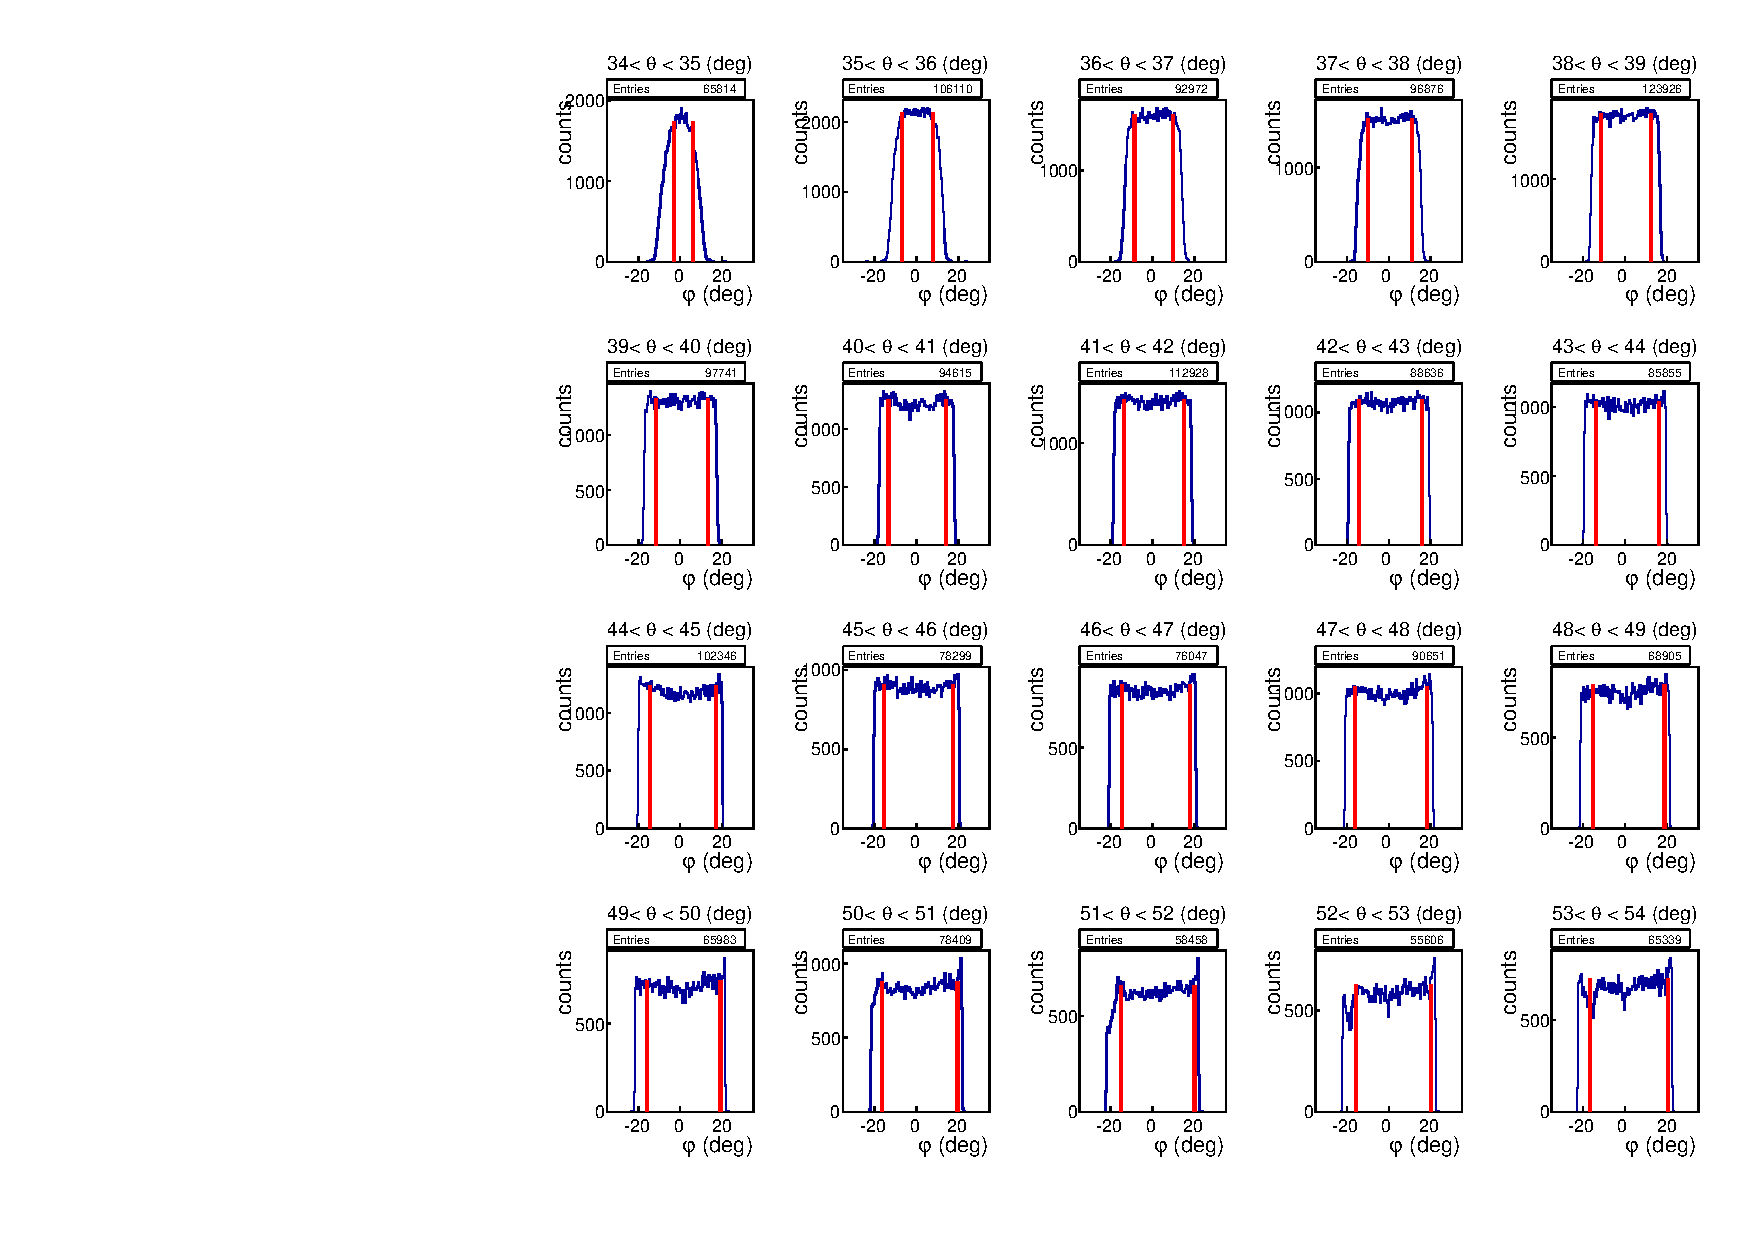
\includegraphics[width=7.5cm]{pictures/other_cuts/fiduch/el_fid_1dim_s6_2.pdf}}
\fbox{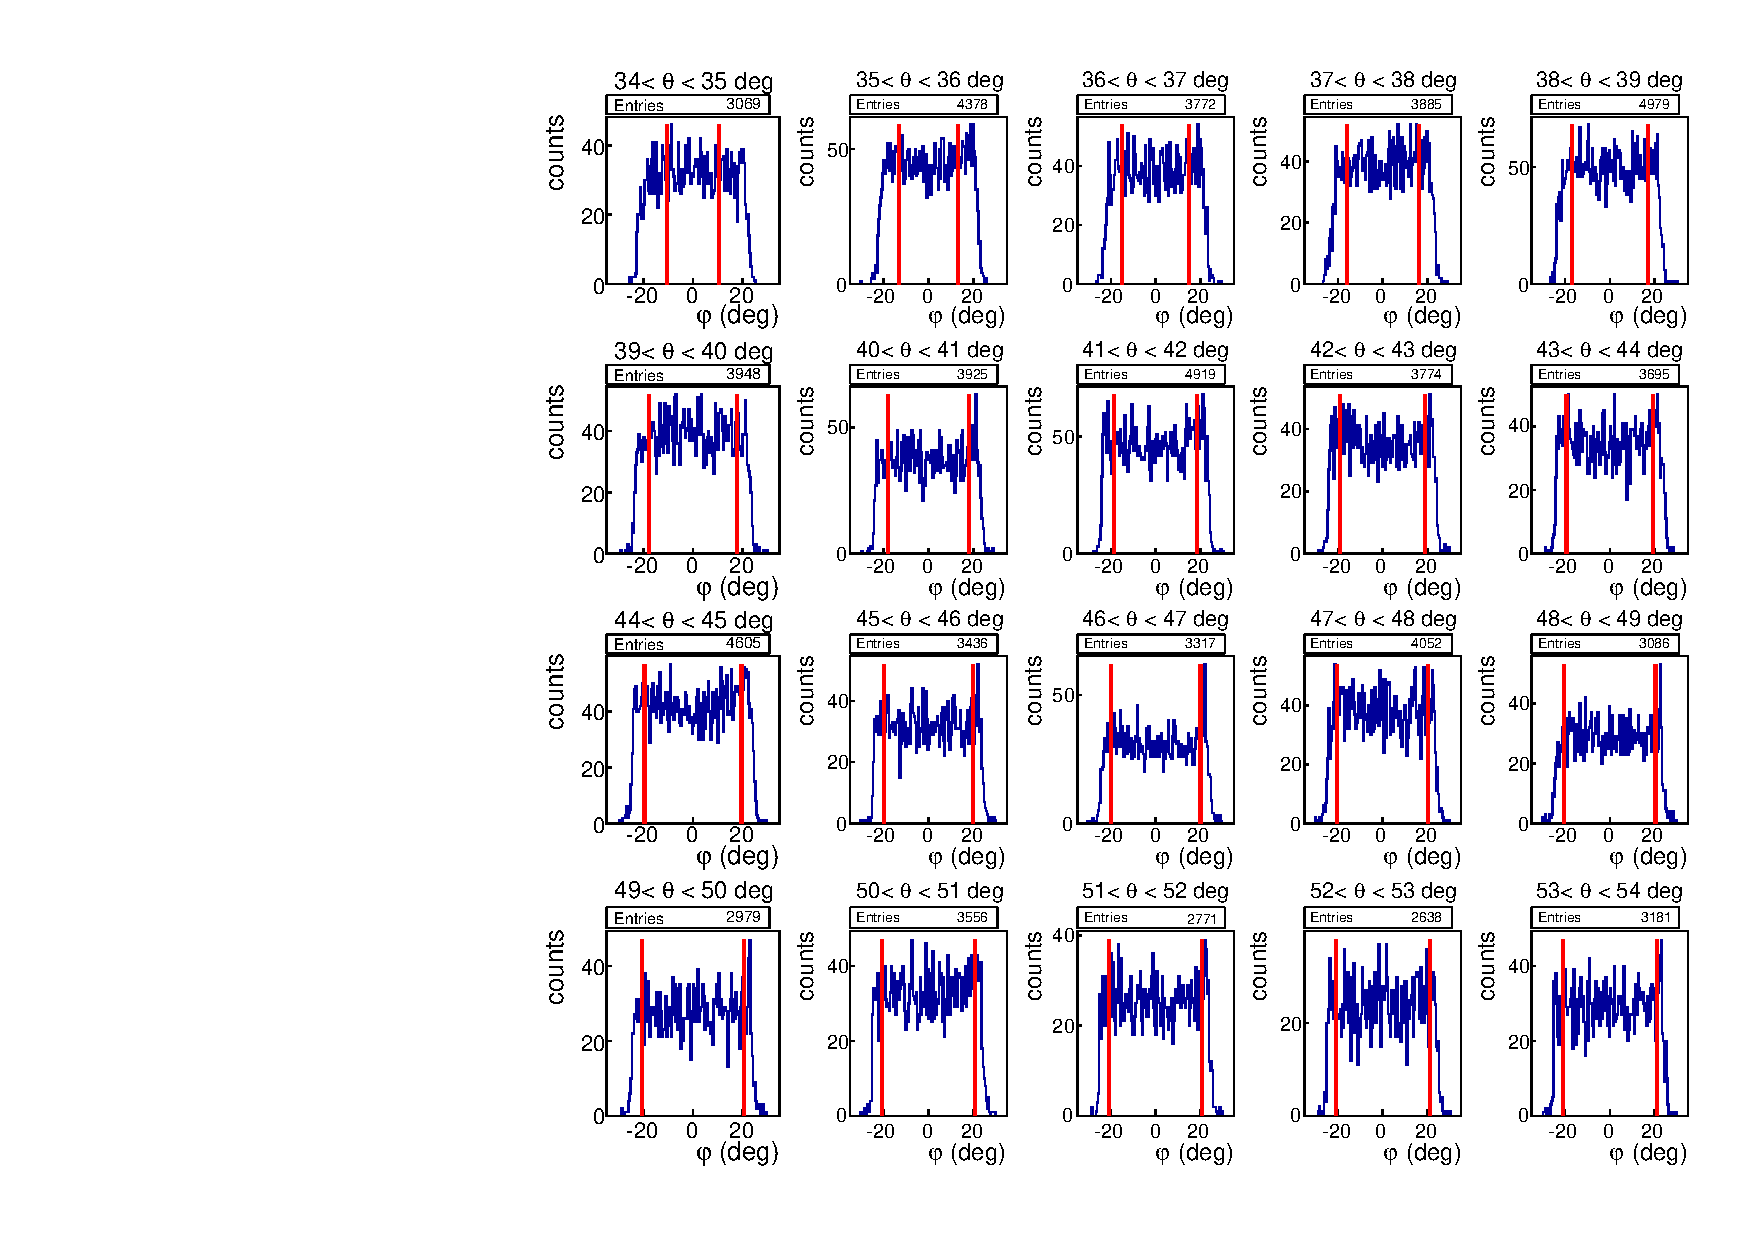
\includegraphics[width=7.5cm]{pictures/other_cuts/fiduch/pim_fid_1dim_s1_3.pdf}}
\caption{\small $\varphi$-event distributions for electrons (left plot) and $\pi^{-}$ (right plot). Electrons are shown for CLAS sector 6 and a momentum range from 480 MeV to 560 MeV, while $\pi^{-}$ are for sector 3 and a momentum range from 400 MeV to 600 MeV. Various plots represent bins in polar angle $\theta$. Events between the red lines are selected for the analysis. \label{fig:fiduch_negative_1d}}
\end{center}
\end{figure}


\begin{figure}[htp]
\begin{center}
\begin{minipage}{.49\textwidth}
\framebox{
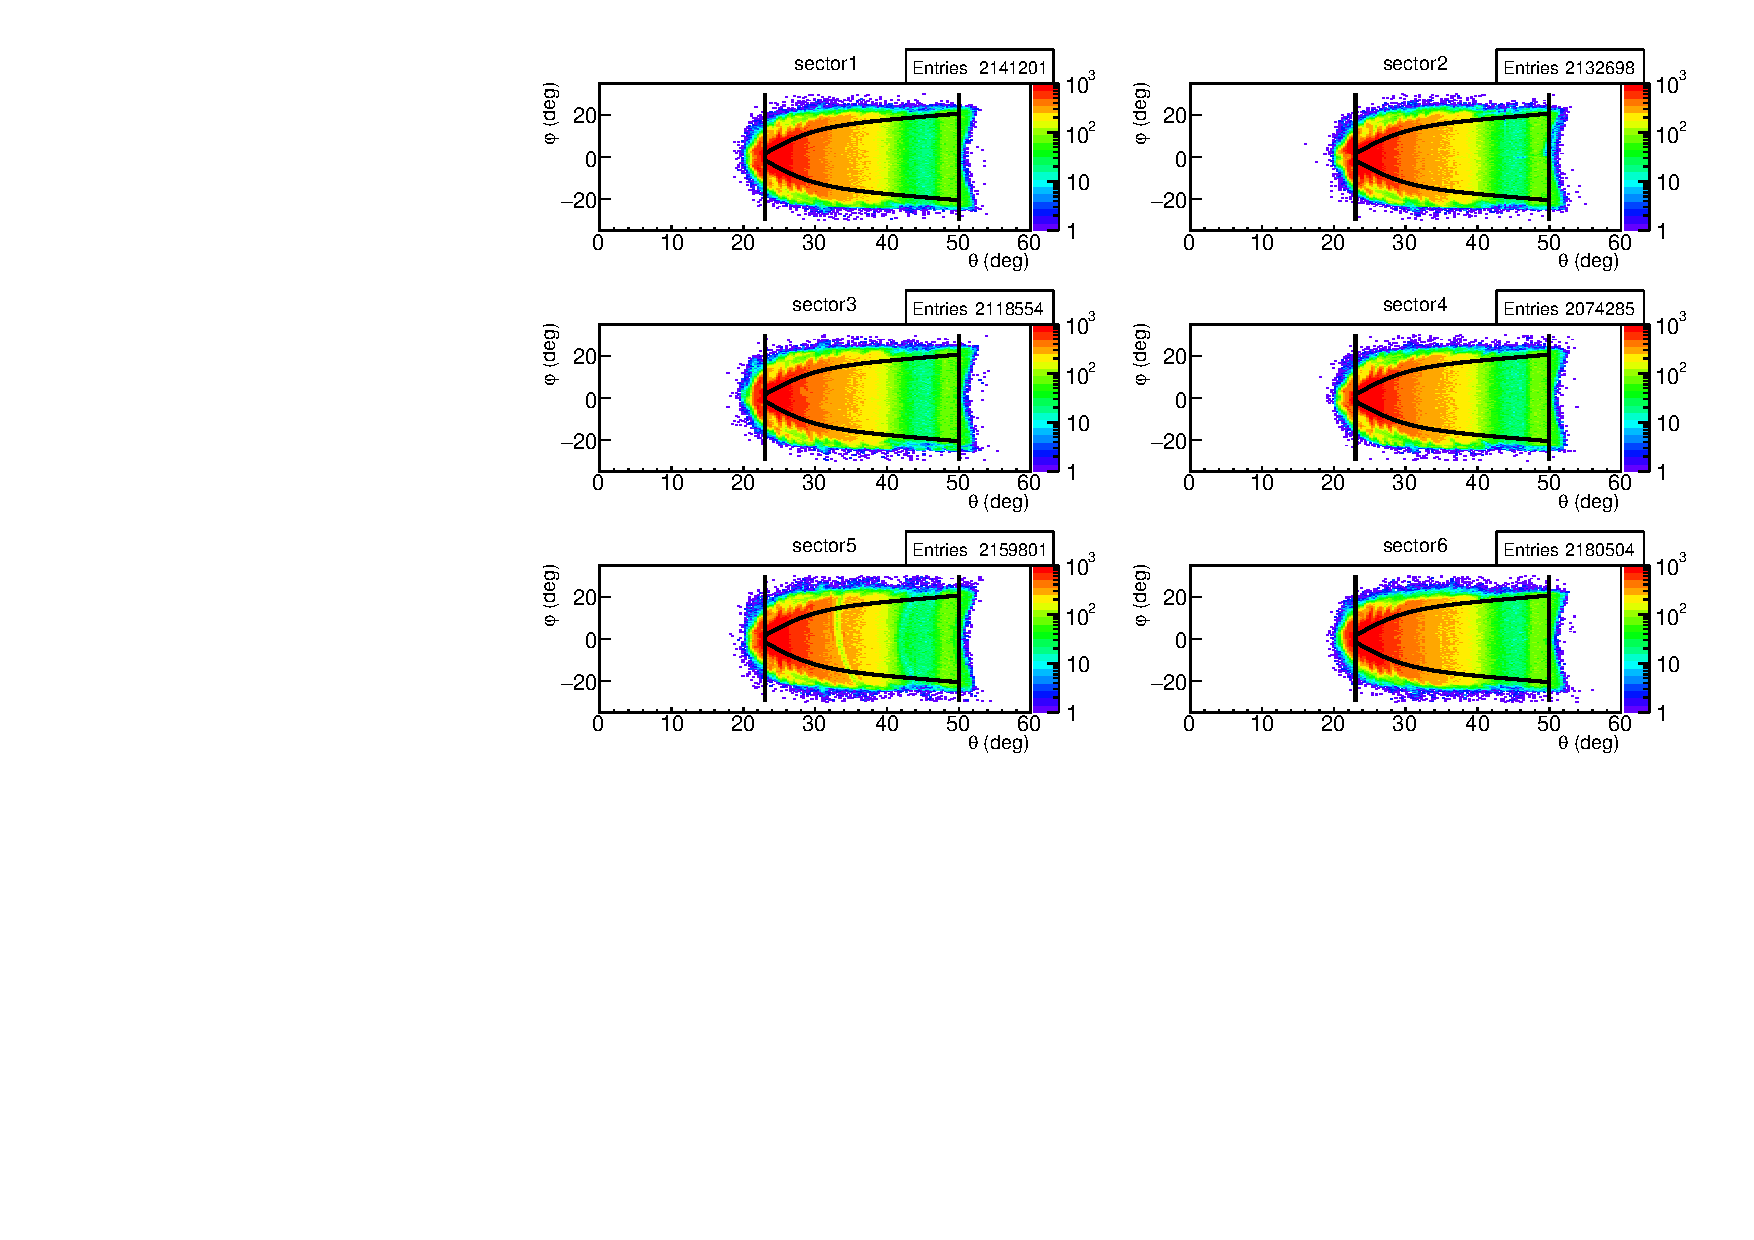
\includegraphics[width=7.6cm]{pictures/other_cuts/fiduch/el_fid_2dim_9.pdf}
}
\end{minipage}
\begin{minipage}{.49\textwidth}
\framebox{
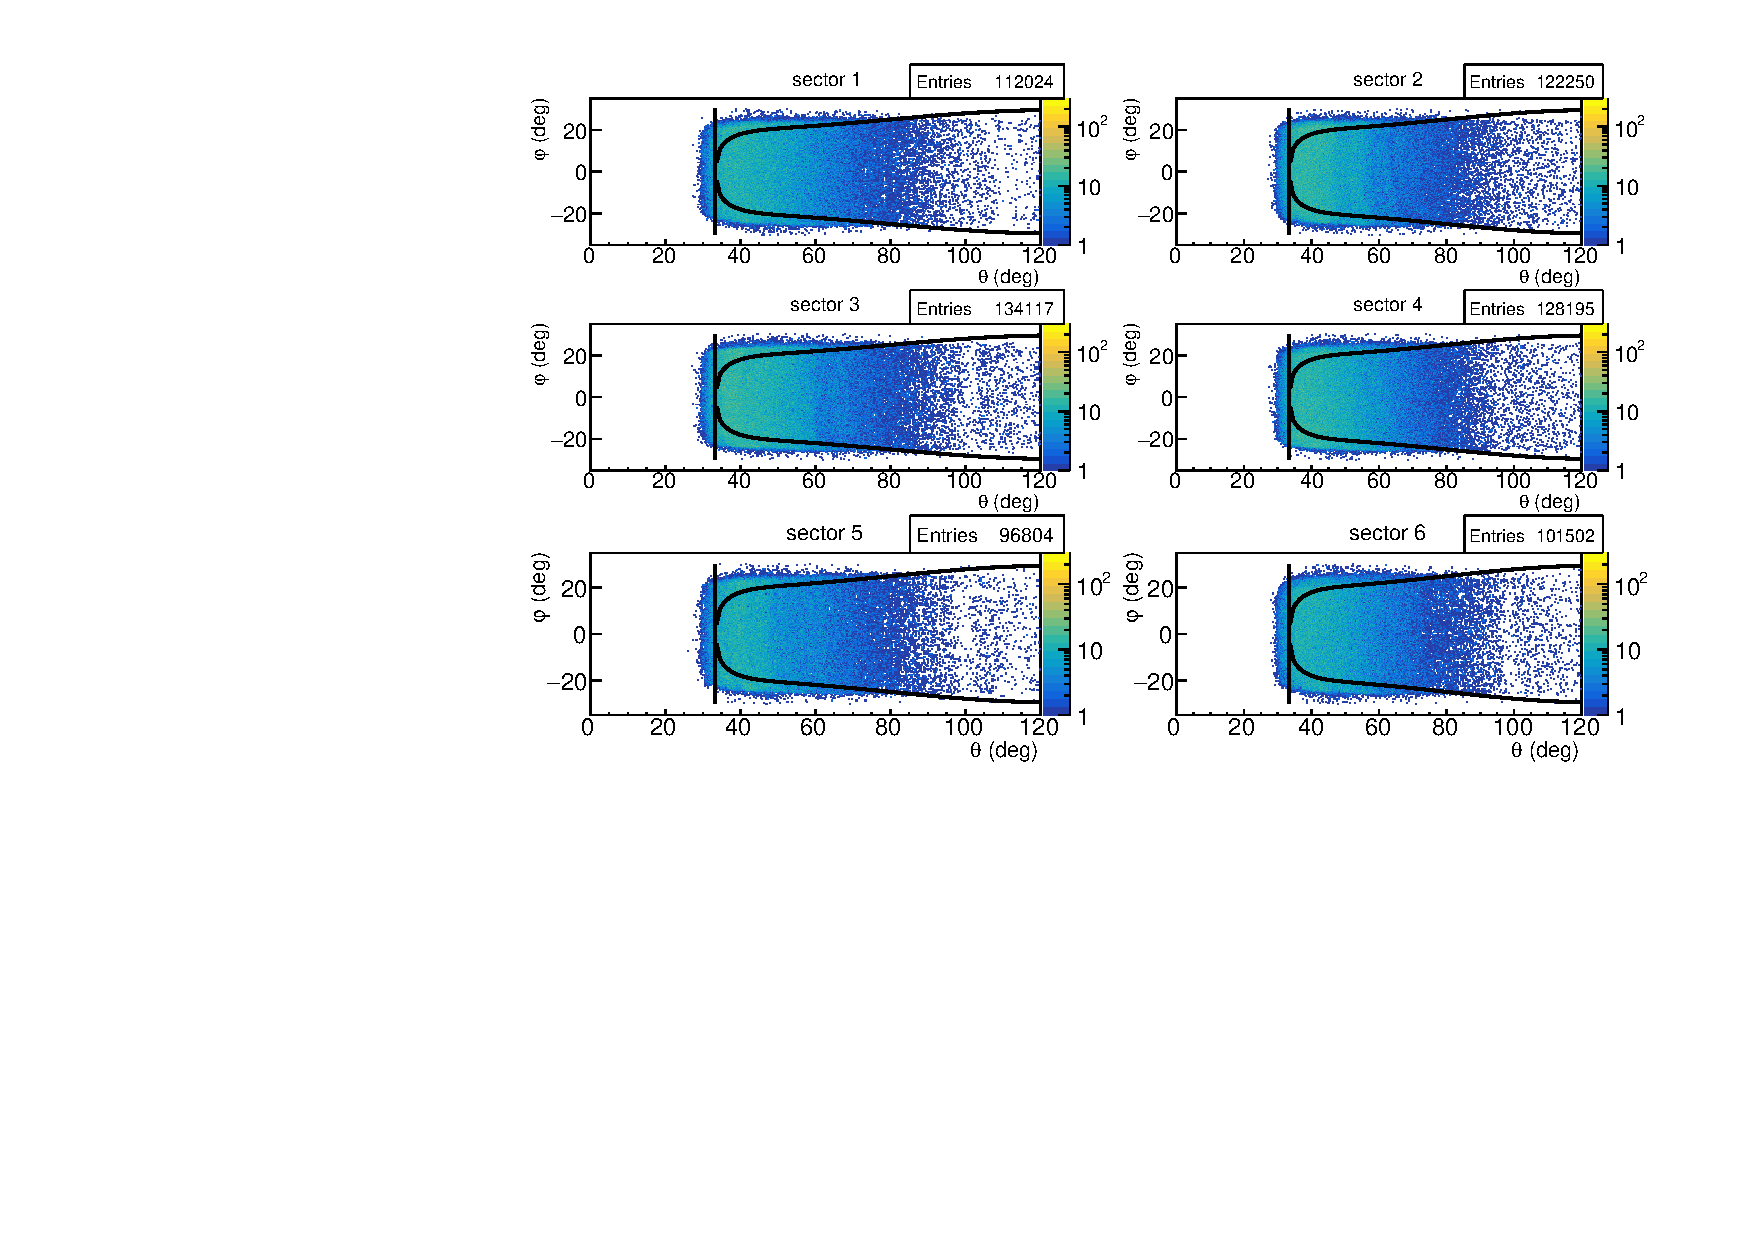
\includegraphics[width=7.6cm]{pictures/other_cuts/fiduch/pim_fid_2dim_2.pdf}
}
\end{minipage}
\caption{\small $\varphi$ versus $\theta$ distributions for electrons with momenta from 1120 MeV to 1200 MeV (left frame) and $\pi^{-}$ with momentuma from 400 MeV to 600 MeV (right frame) for all six CLAS sectors. Curves show the applied fiducial cuts, vertical lines stand for minimum and maximum $\theta$ cuts. \label{fig:eother_cuts_negative_fiduch_2d}}
\end{center}
\end{figure}







\begin{figure}[htp]
\begin{center}
\frame{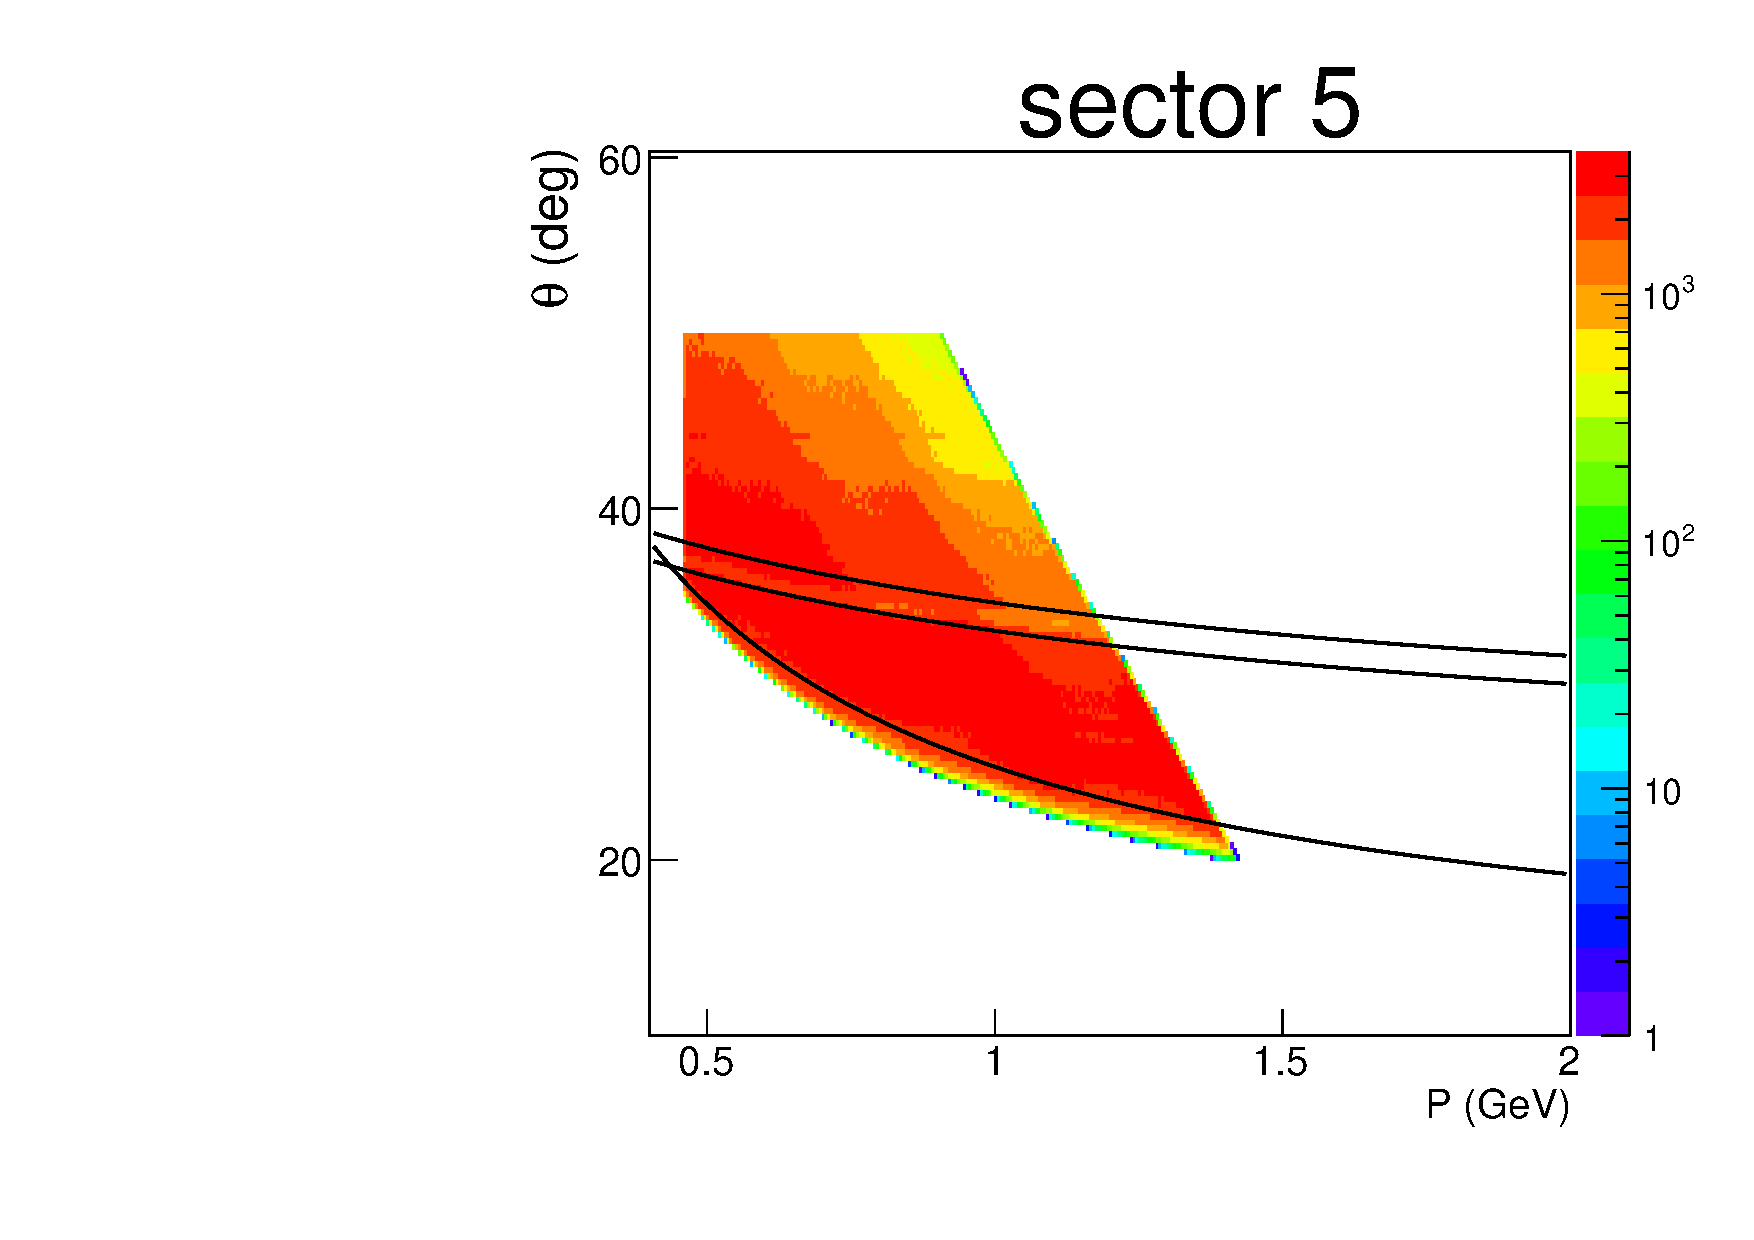
\includegraphics[width=5cm]{pictures/other_cuts/fiduch/th_vs_p_el/el_th_vs_p_sector5.pdf}\
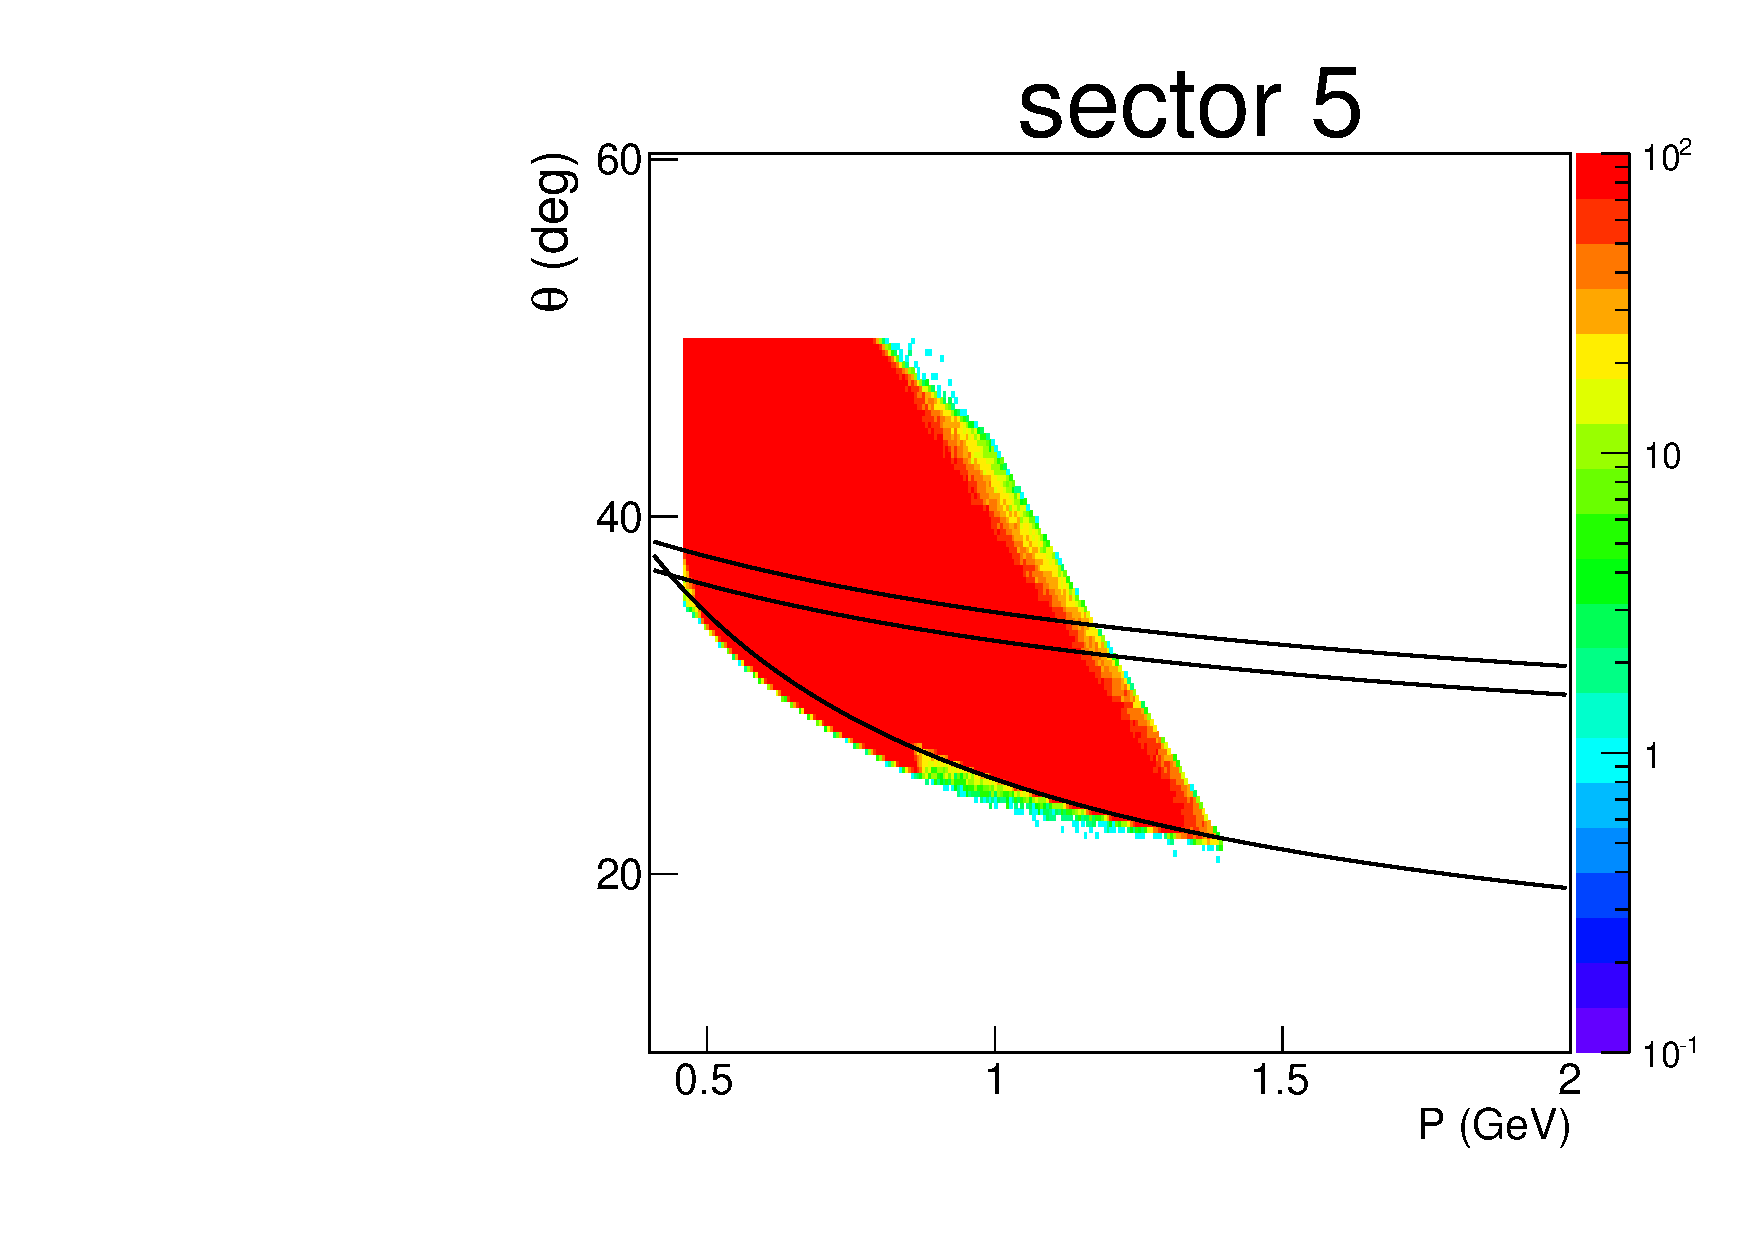
\includegraphics[width=5cm]{pictures/other_cuts/fiduch/th_vs_p_el_sim/el_th_vs_p_sim_sector5.pdf}}
\caption{\small $\theta$ versus momentum distributions for electrons in CLAS sector five. Left plot shows real and right plot Monte Carlo events. Black curves show cuts applied to remove inefficient areas. \label{fig:other_cuts_negaitive_th_vs_p_electronss}}
\end{center}
\end{figure}





\begin{figure}[htp]
\begin{center}
%\begin{framed}
\begin{minipage}{.99\textwidth}
\begin{framed}
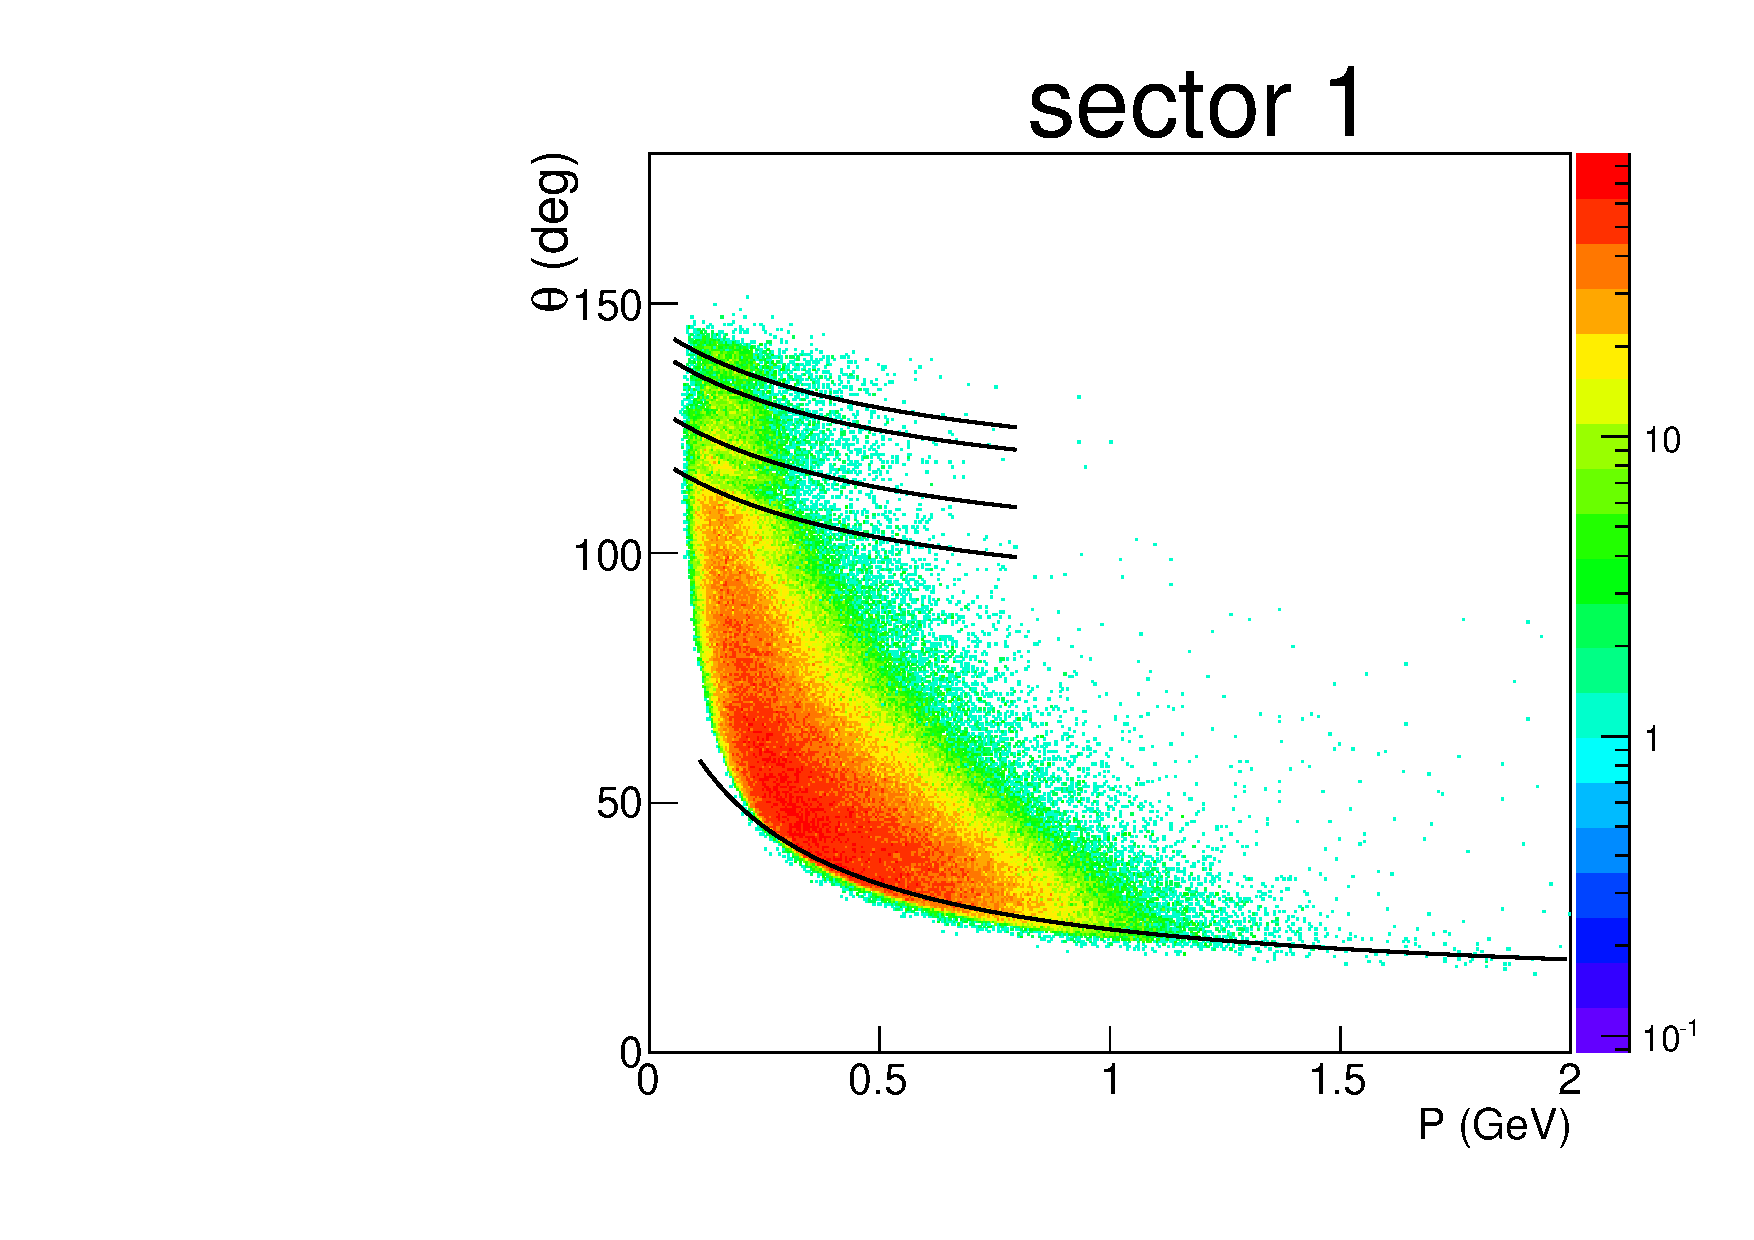
\includegraphics[width=5cm]{pictures/other_cuts/fiduch/th_vs_p_pim/pim_th_vs_p_sector1.pdf}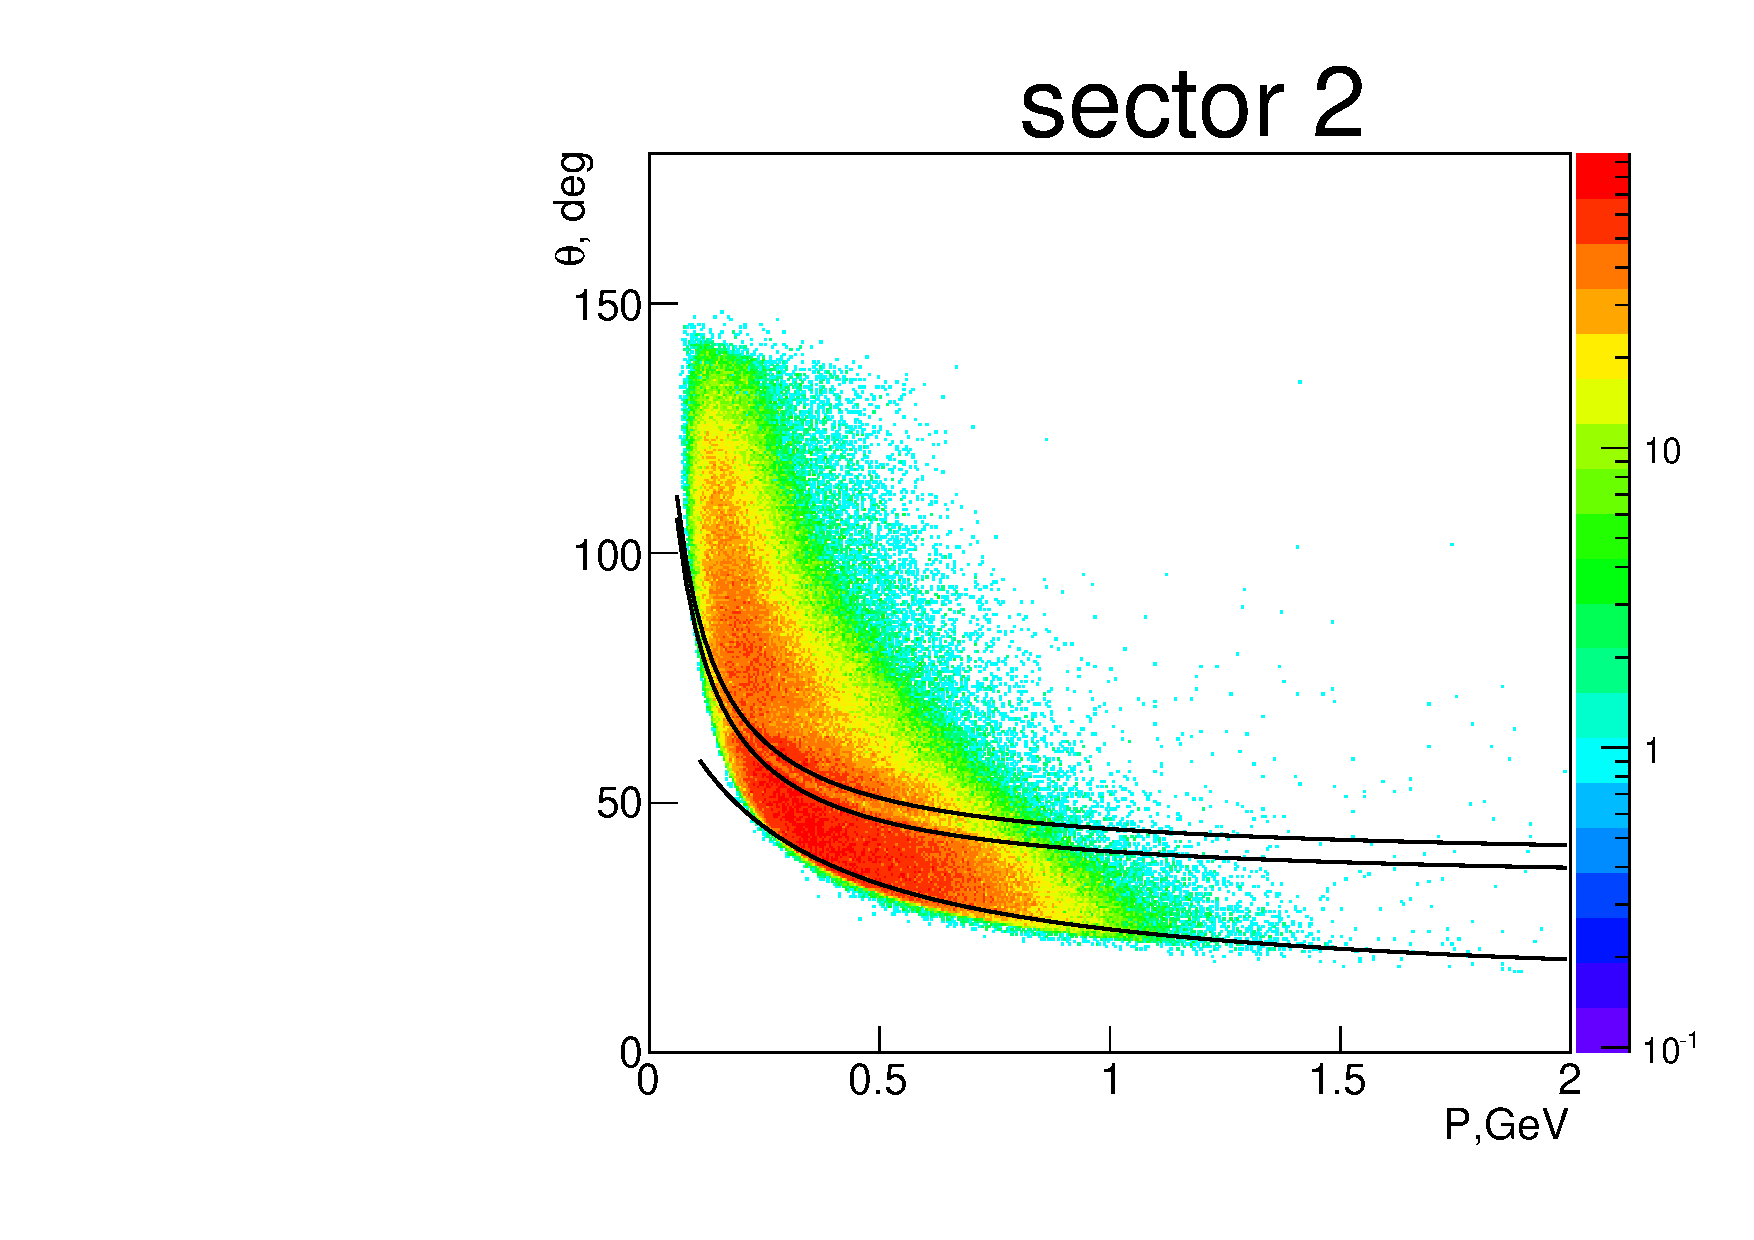
\includegraphics[width=5cm]{pictures/other_cuts/fiduch/th_vs_p_pim/pim_th_vs_p_sector2.pdf}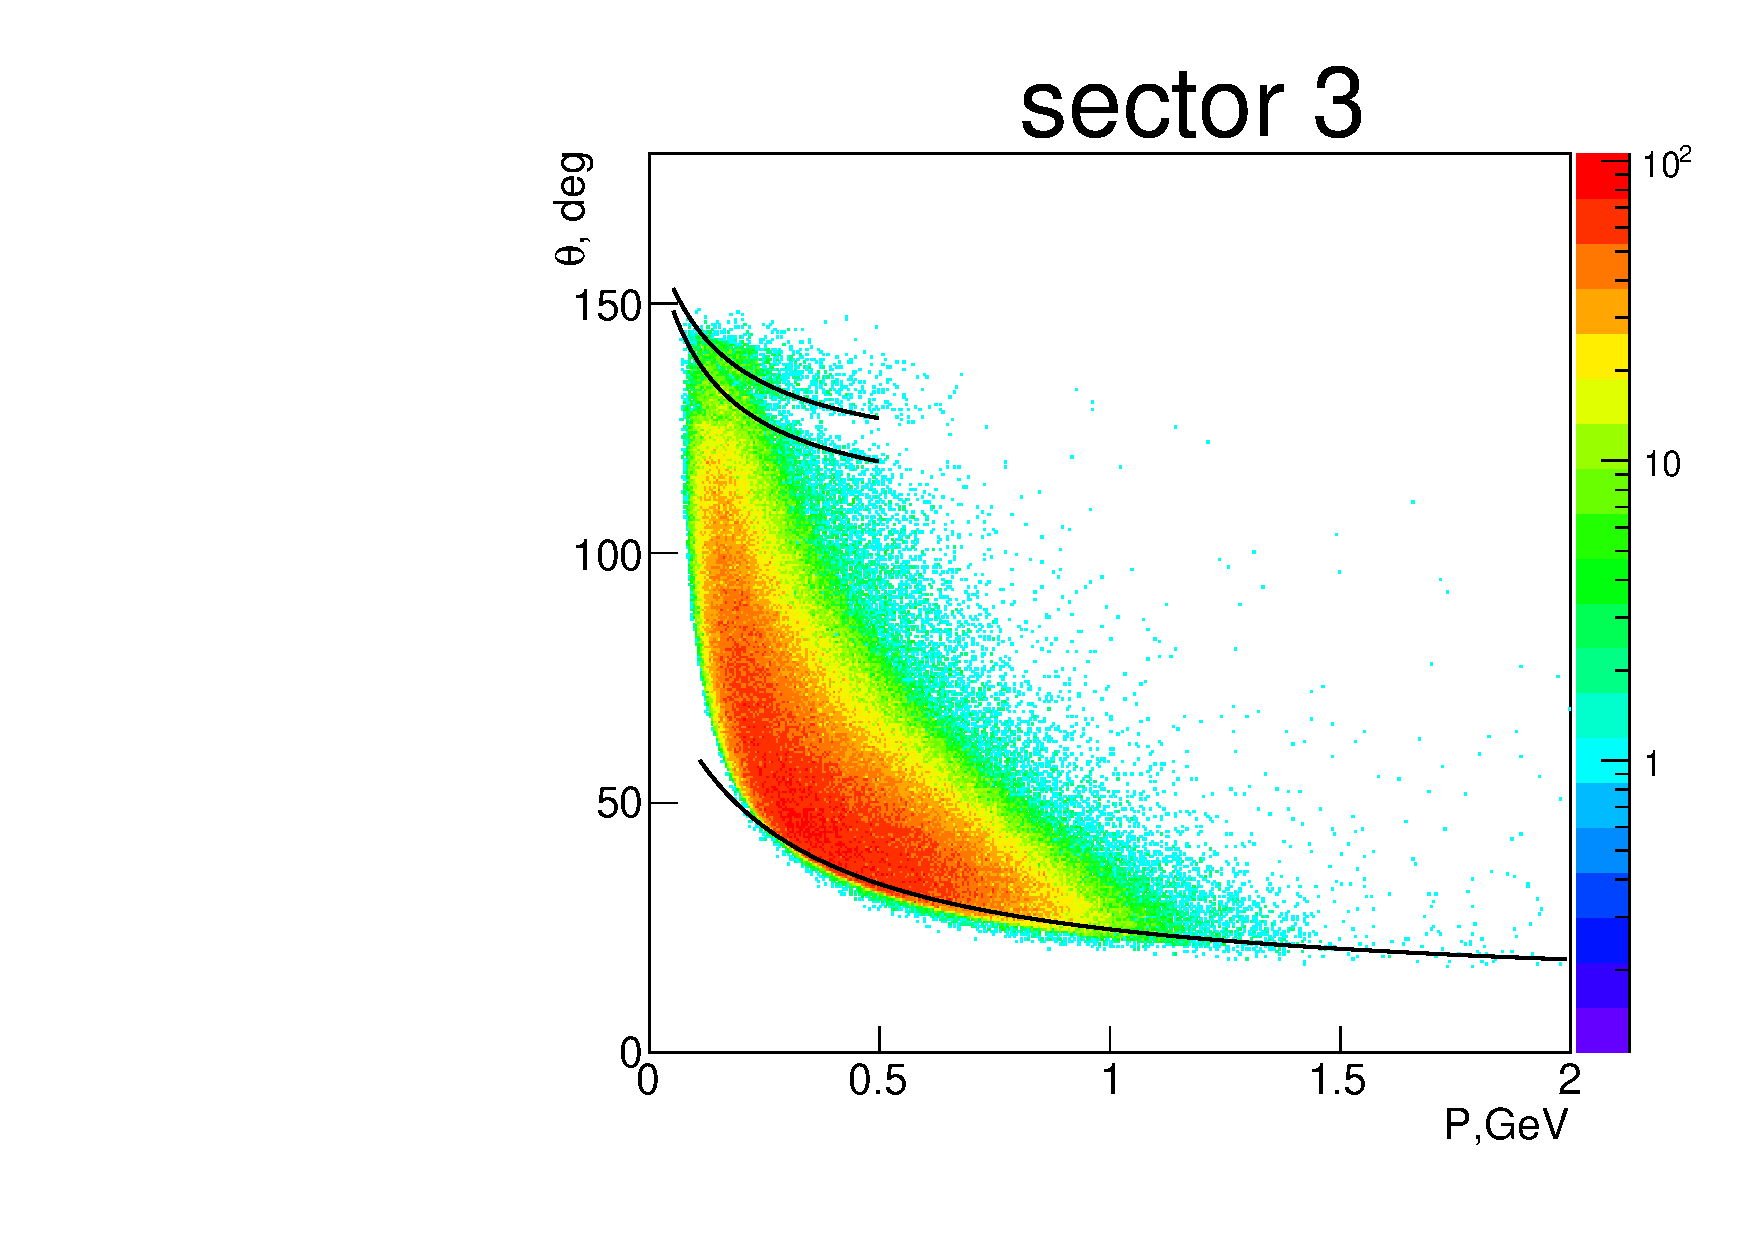
\includegraphics[width=5cm]{pictures/other_cuts/fiduch/th_vs_p_pim/pim_th_vs_p_sector3.pdf}
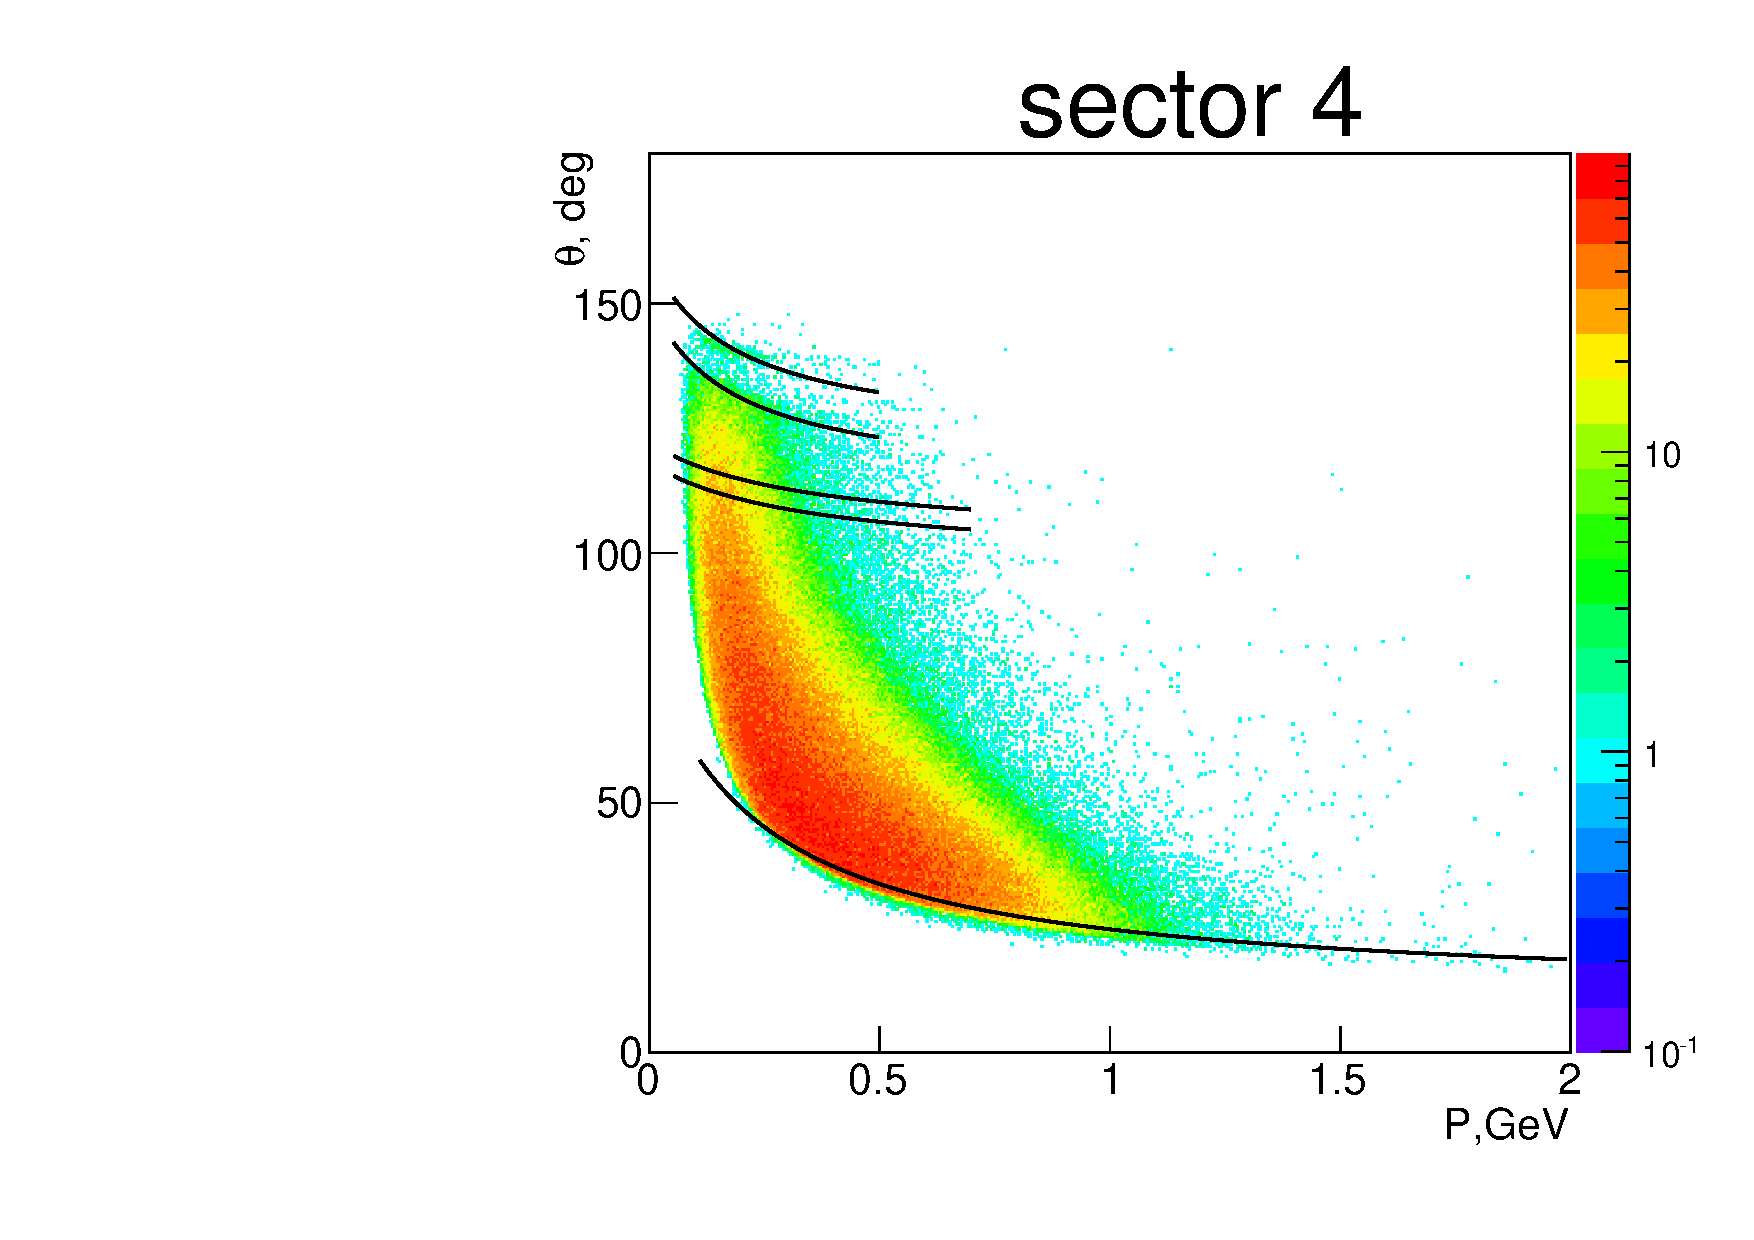
\includegraphics[width=5cm]{pictures/other_cuts/fiduch/th_vs_p_pim/pim_th_vs_p_sector4.pdf}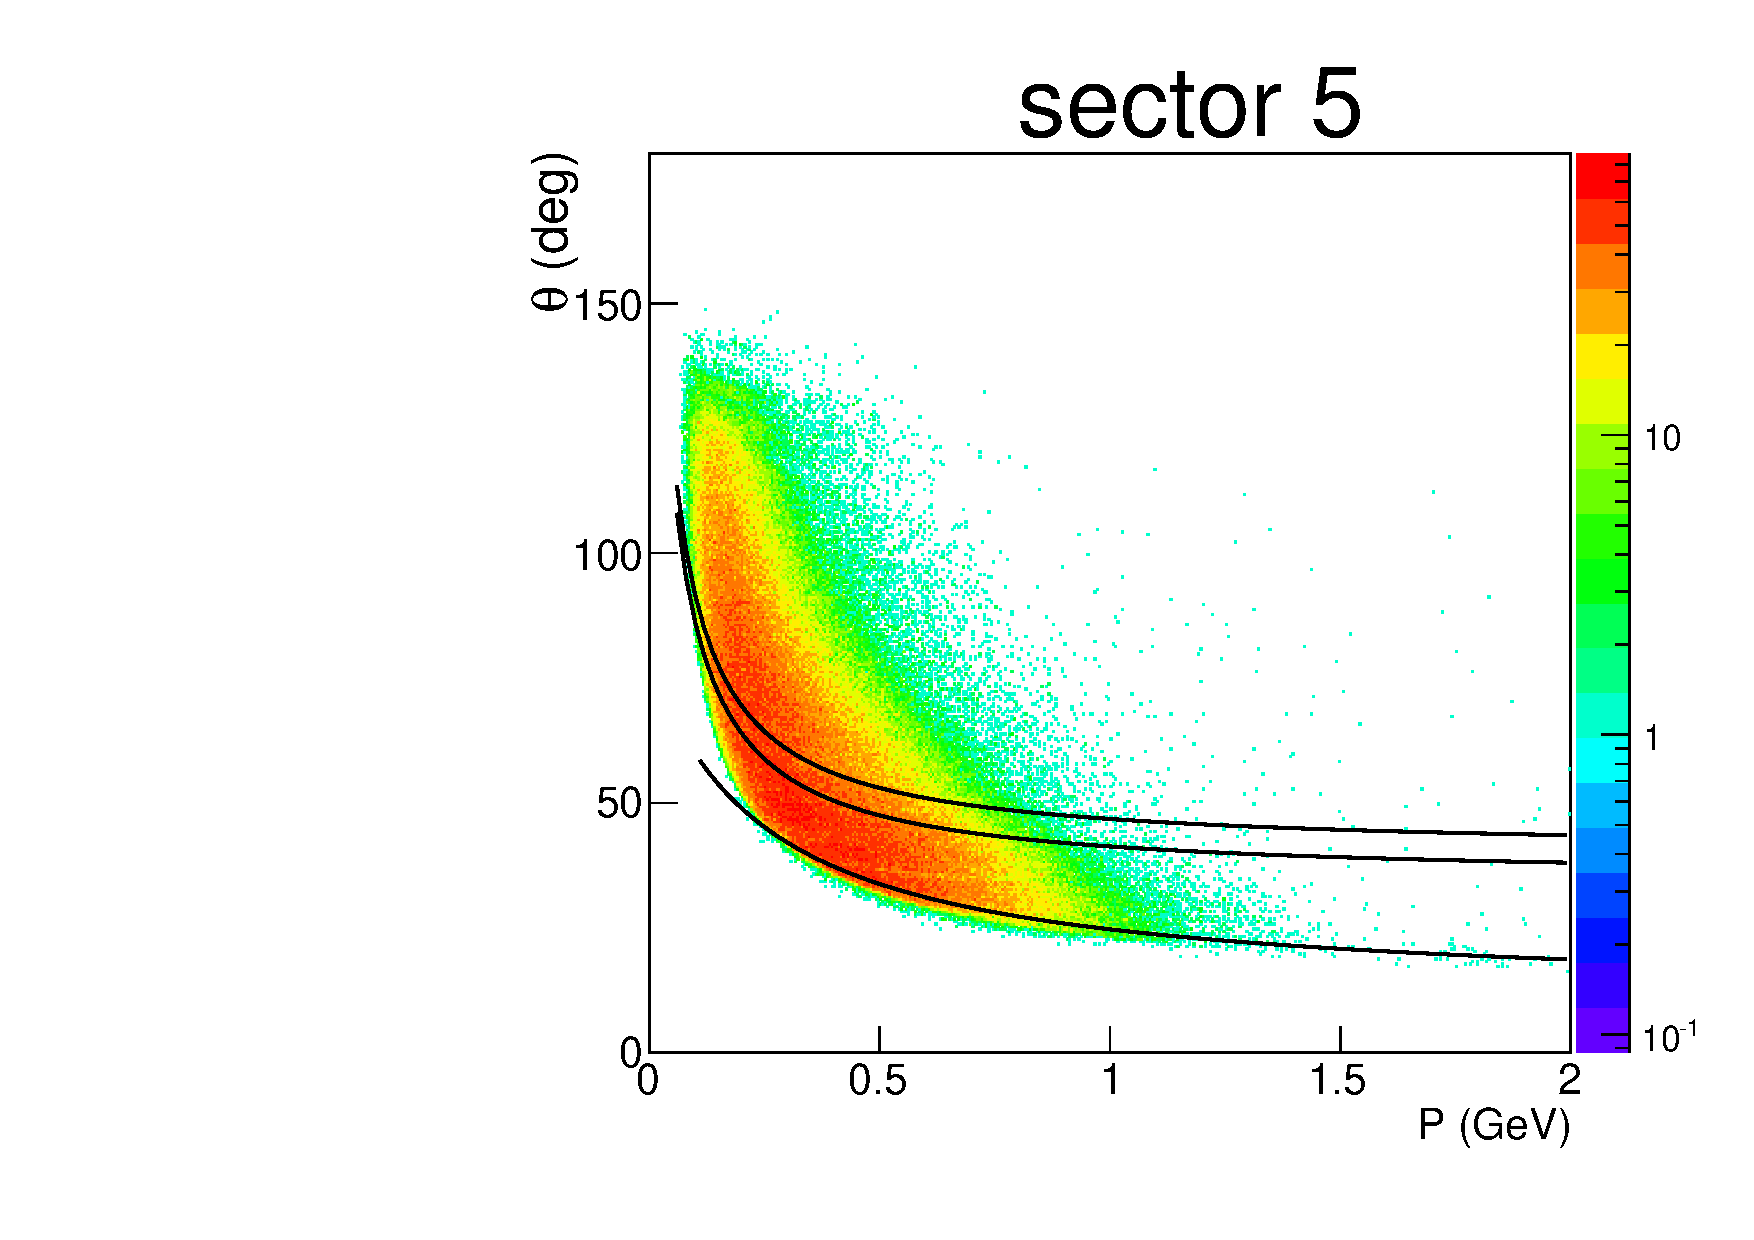
\includegraphics[width=5cm]{pictures/other_cuts/fiduch/th_vs_p_pim/pim_th_vs_p_sector5.pdf}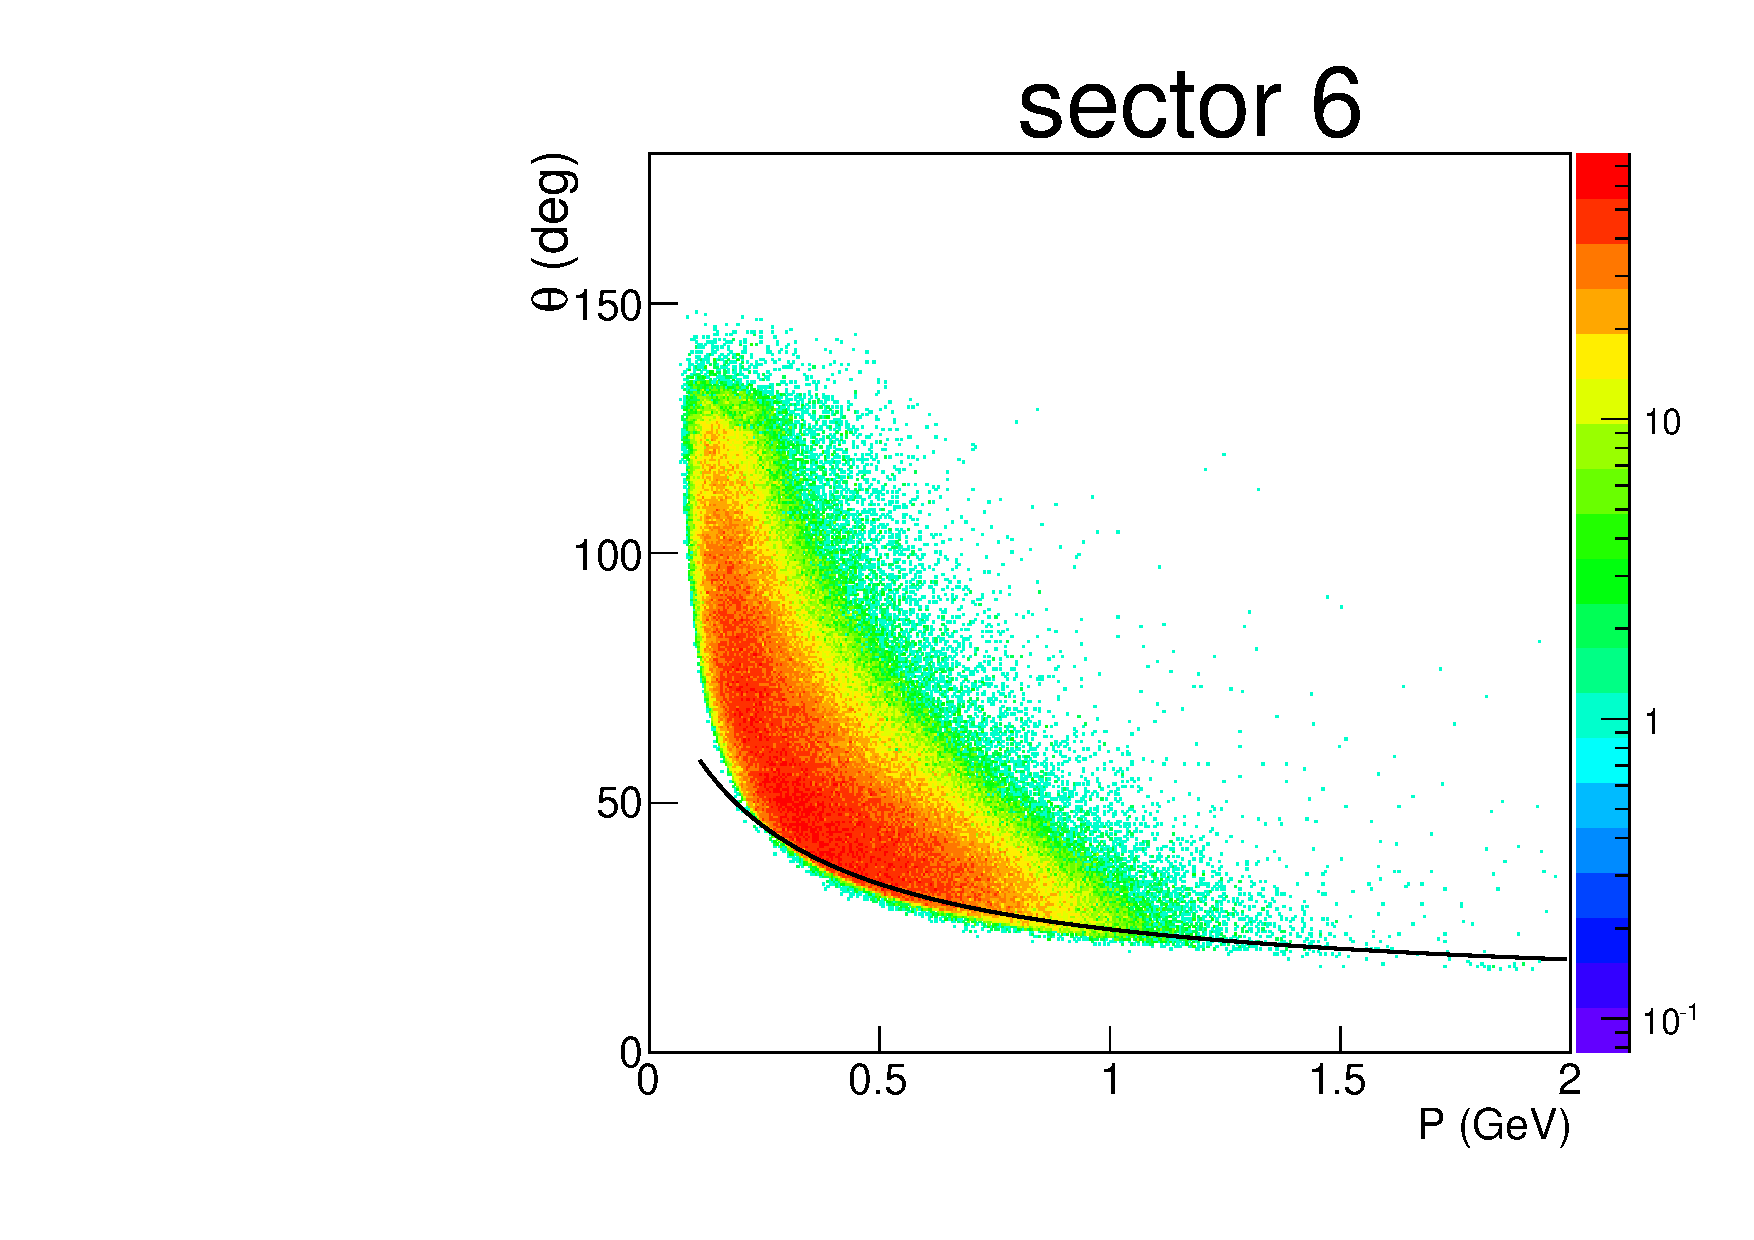
\includegraphics[width=5cm]{pictures/other_cuts/fiduch/th_vs_p_pim/pim_th_vs_p_sector6.pdf}
\end{framed}
\end{minipage}
\begin{minipage}{.99\textwidth}
\begin{framed}
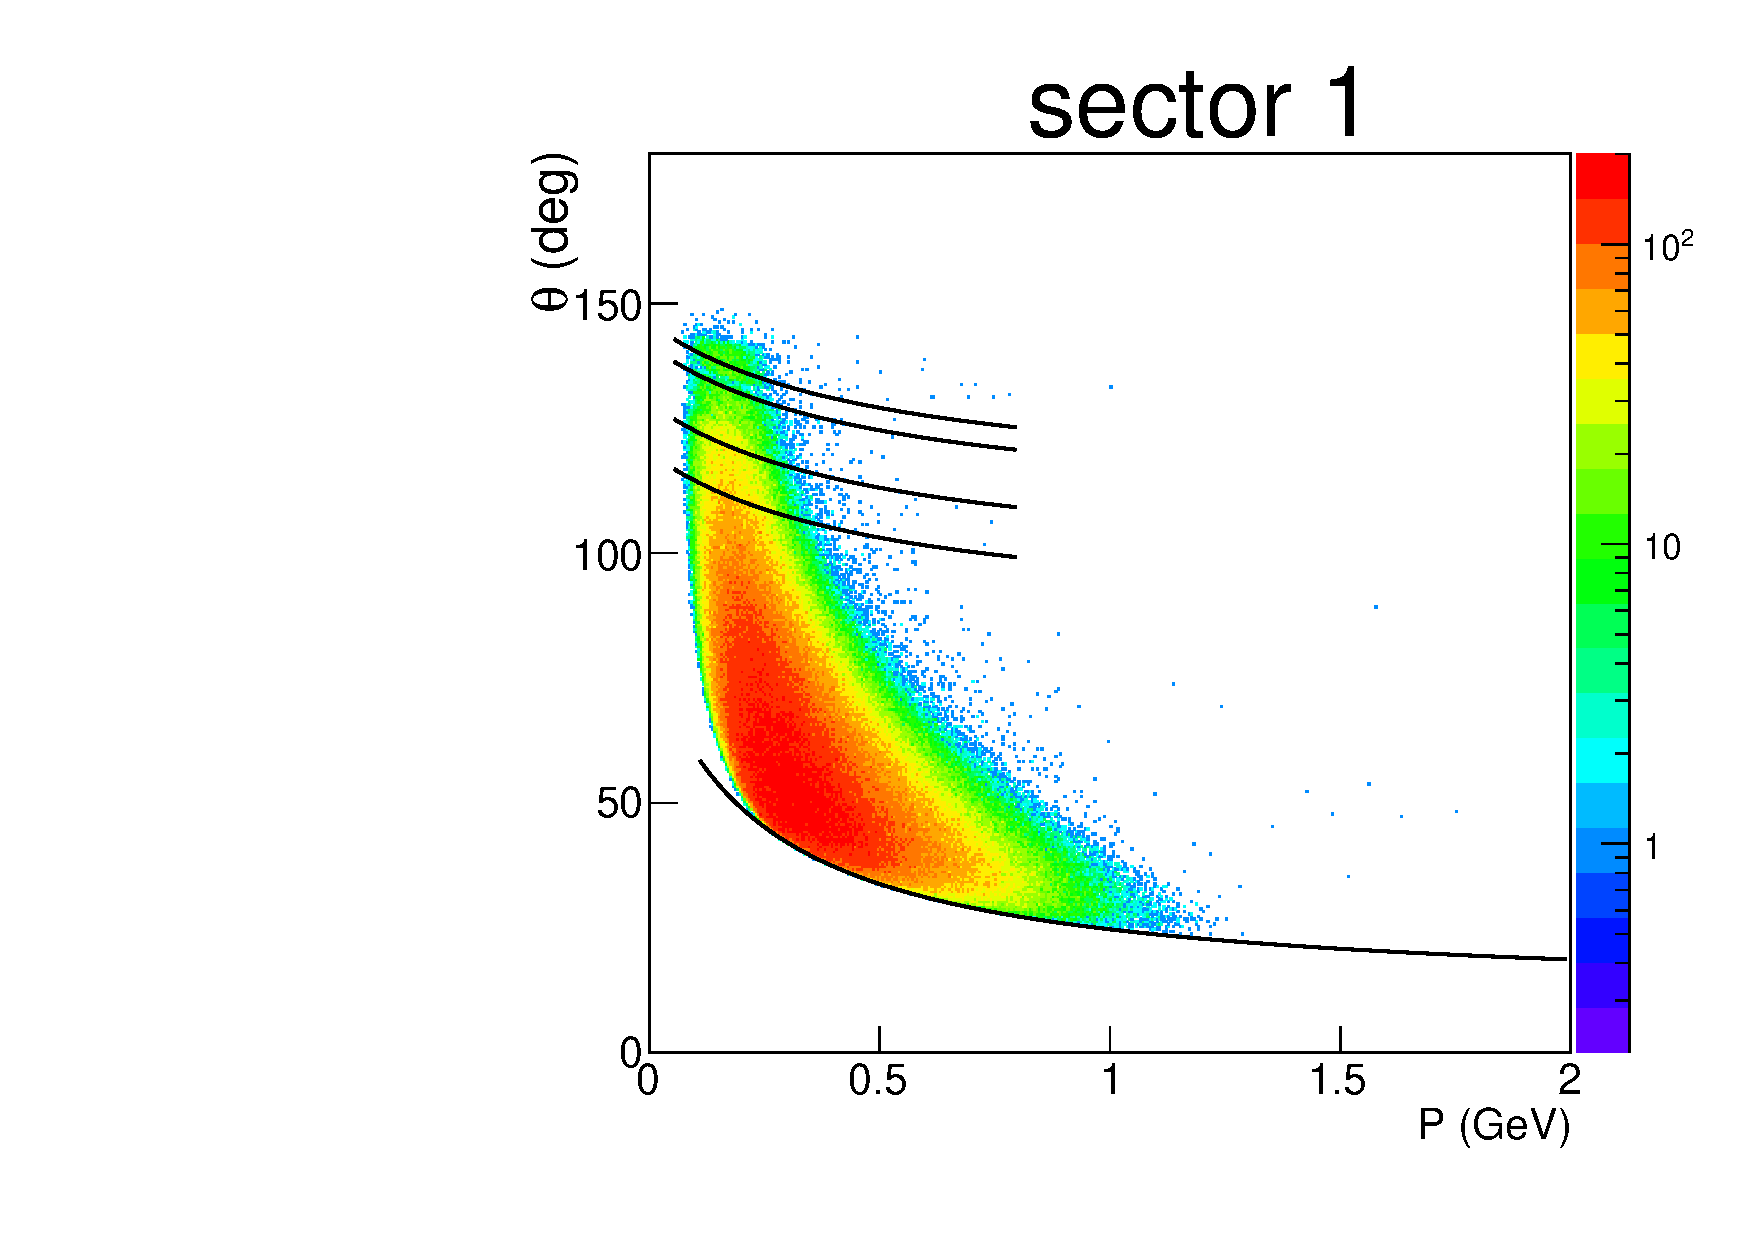
\includegraphics[width=5cm]{pictures/other_cuts/fiduch/th_vs_p_pim_sim/pim_th_vs_p_sim_sector1.pdf}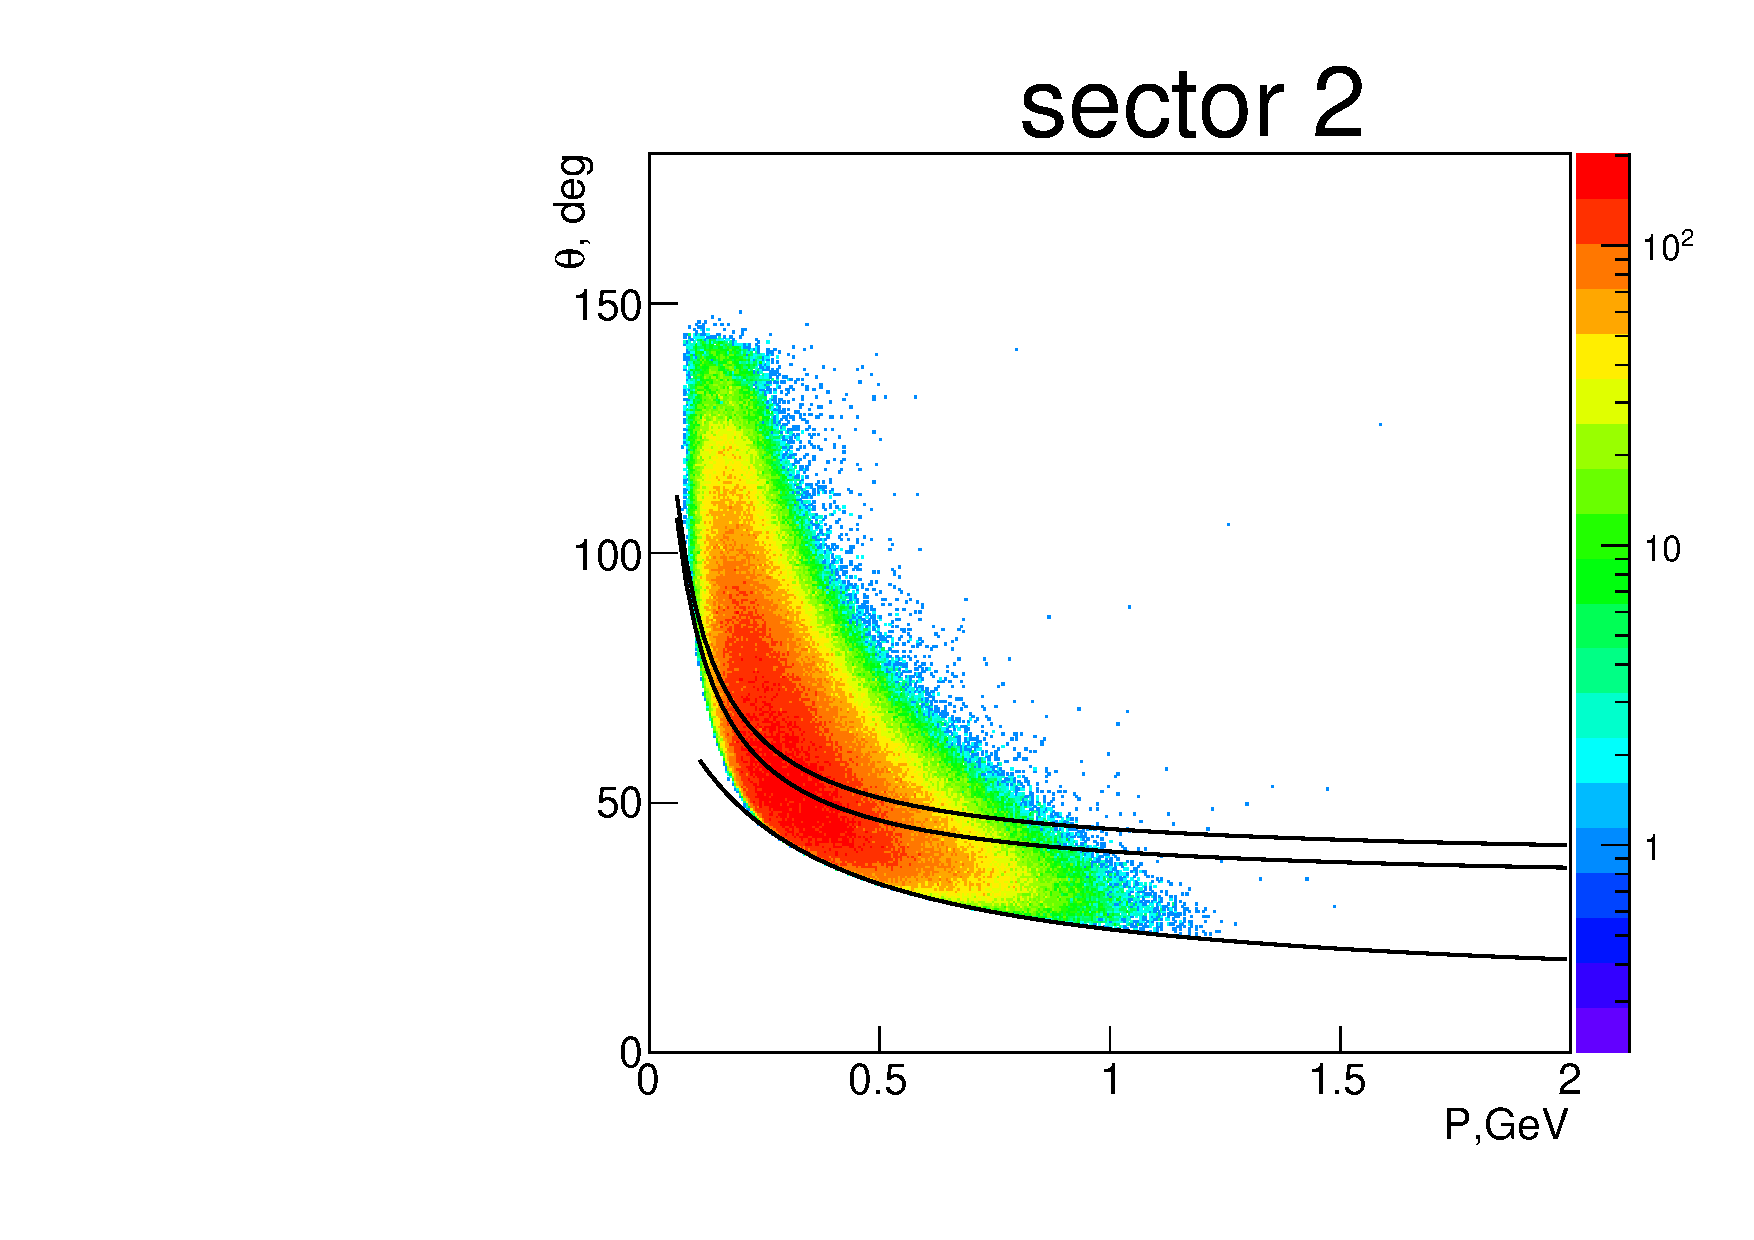
\includegraphics[width=5cm]{pictures/other_cuts/fiduch/th_vs_p_pim_sim/pim_th_vs_p_sim_sector2.pdf}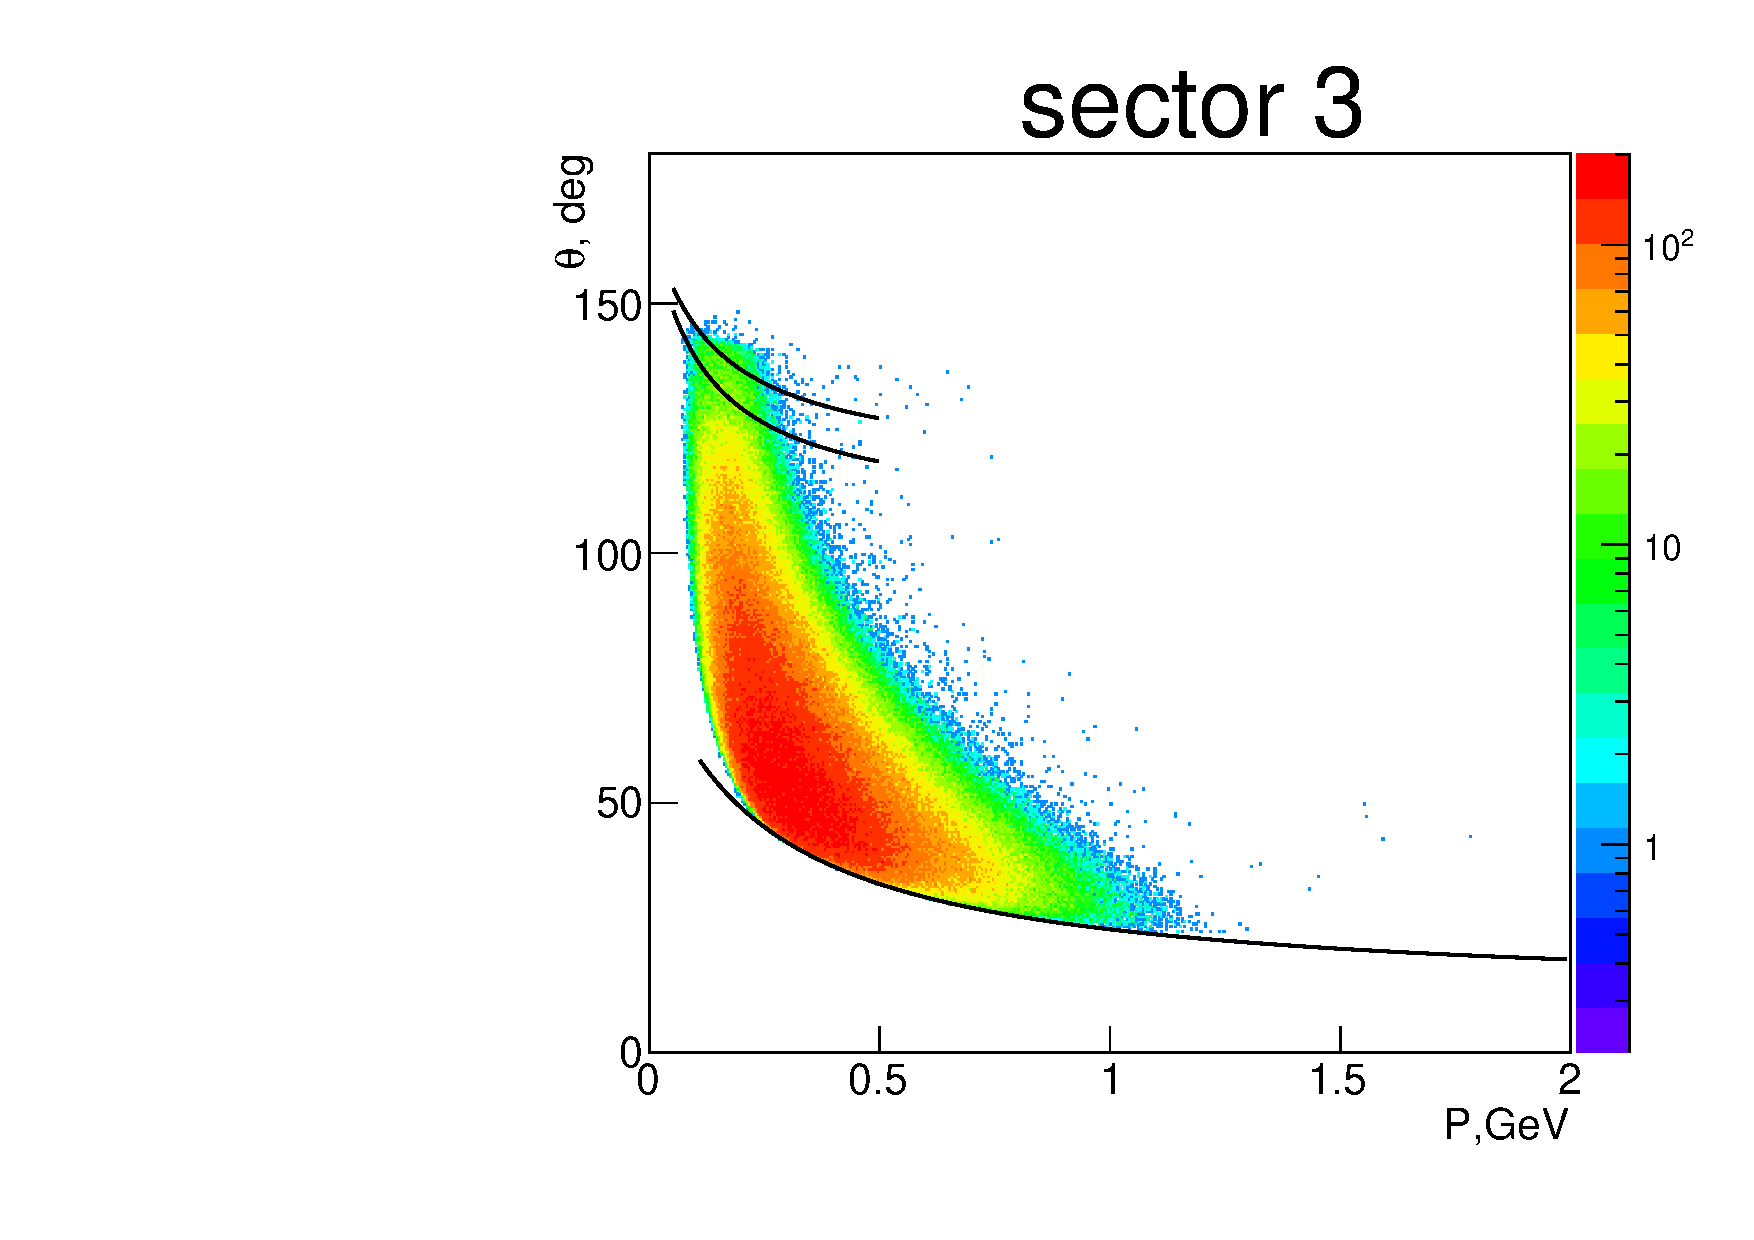
\includegraphics[width=5cm]{pictures/other_cuts/fiduch/th_vs_p_pim_sim/pim_th_vs_p_sim_sector3.pdf}
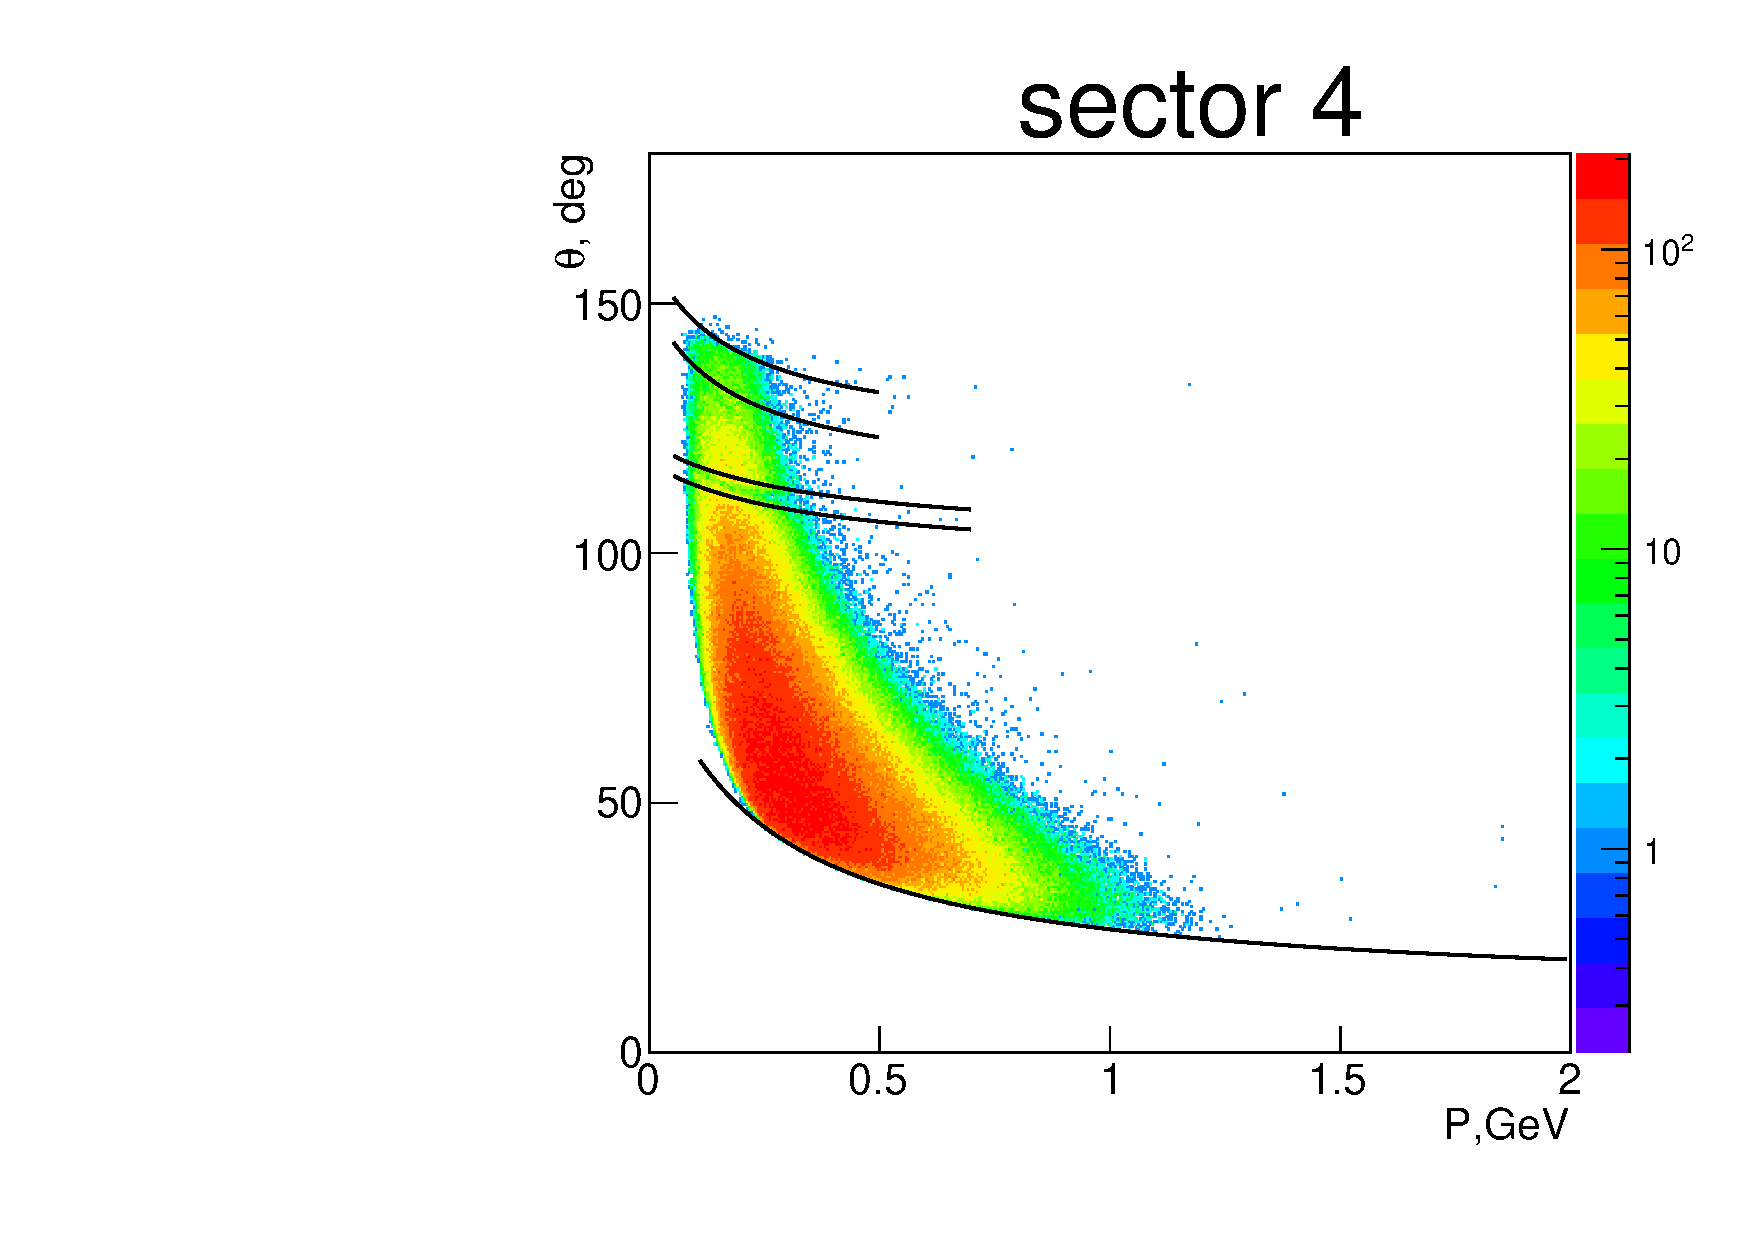
\includegraphics[width=5cm]{pictures/other_cuts/fiduch/th_vs_p_pim_sim/pim_th_vs_p_sim_sector4.pdf}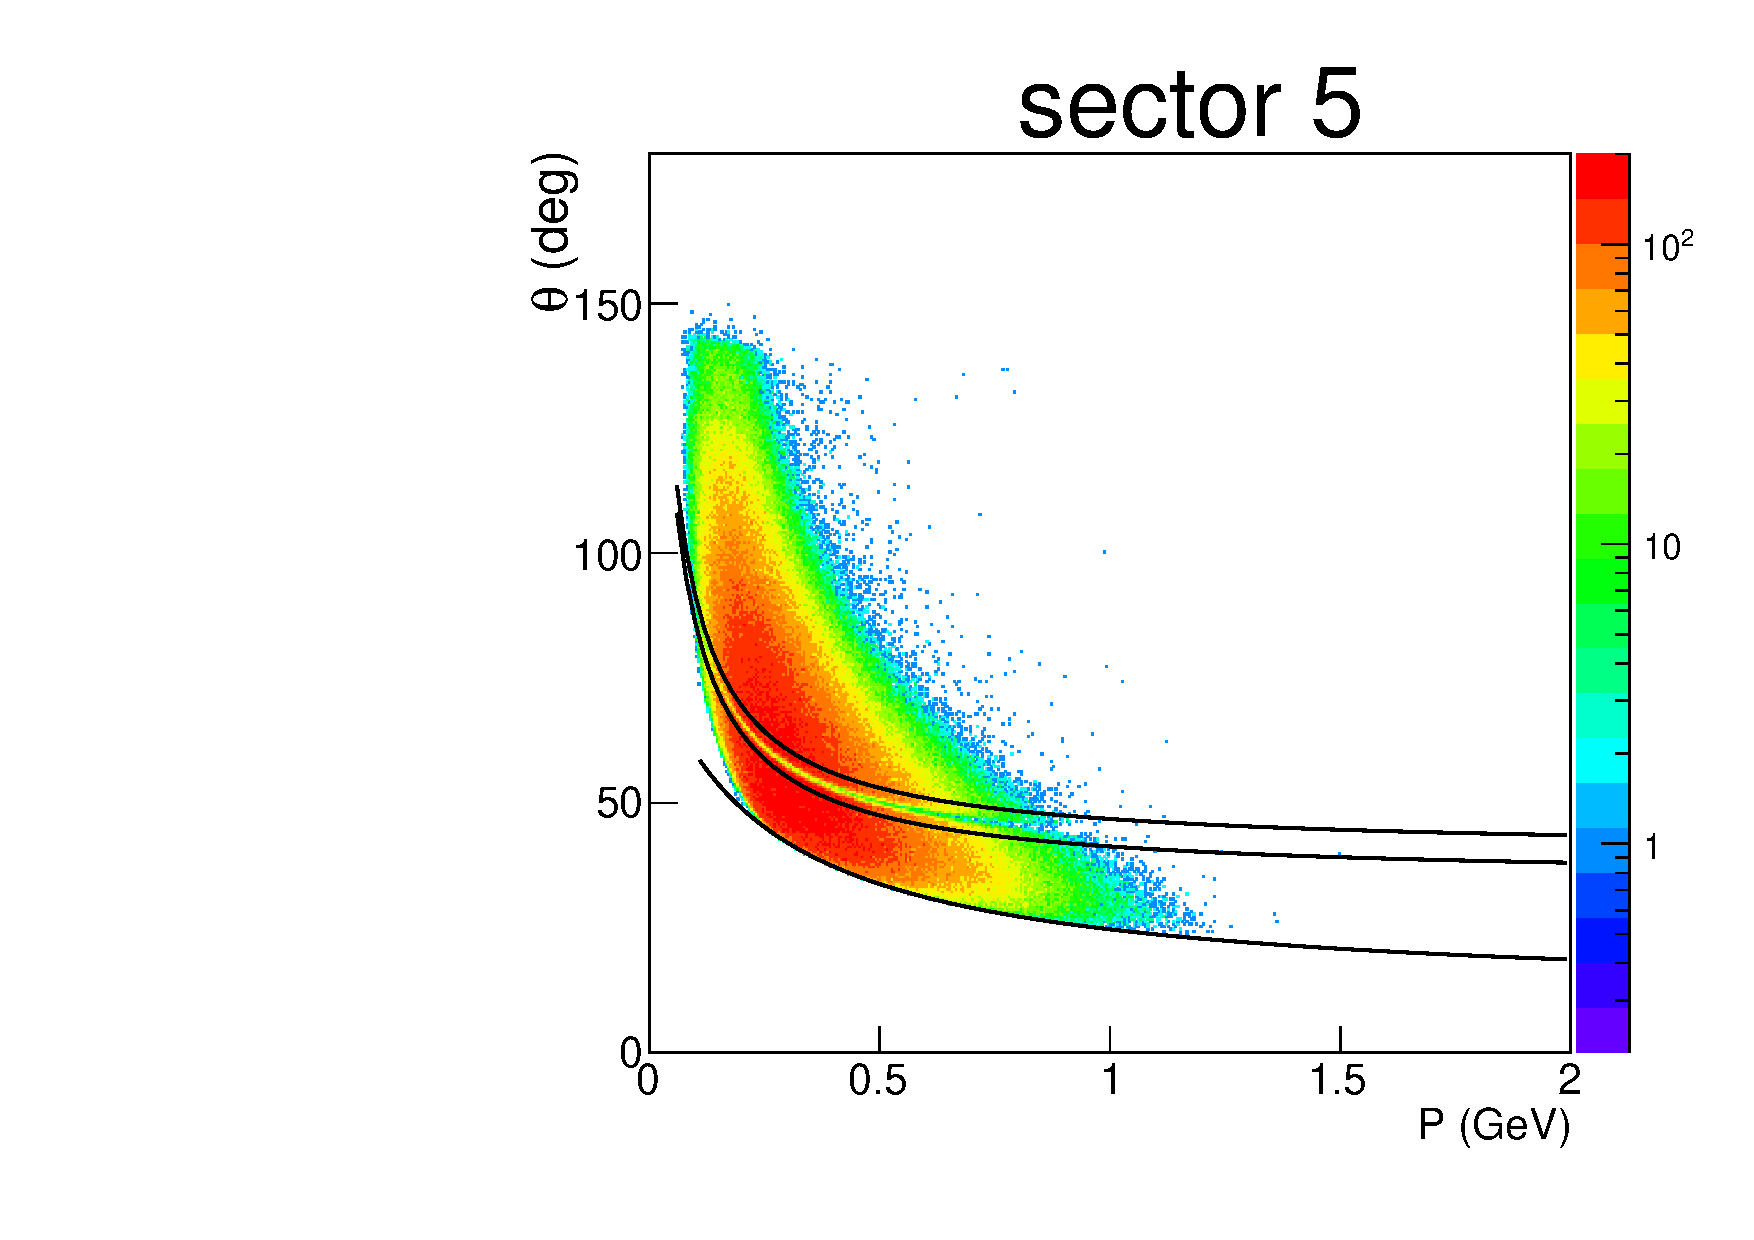
\includegraphics[width=5cm]{pictures/other_cuts/fiduch/th_vs_p_pim_sim/pim_th_vs_p_sim_sector5.pdf}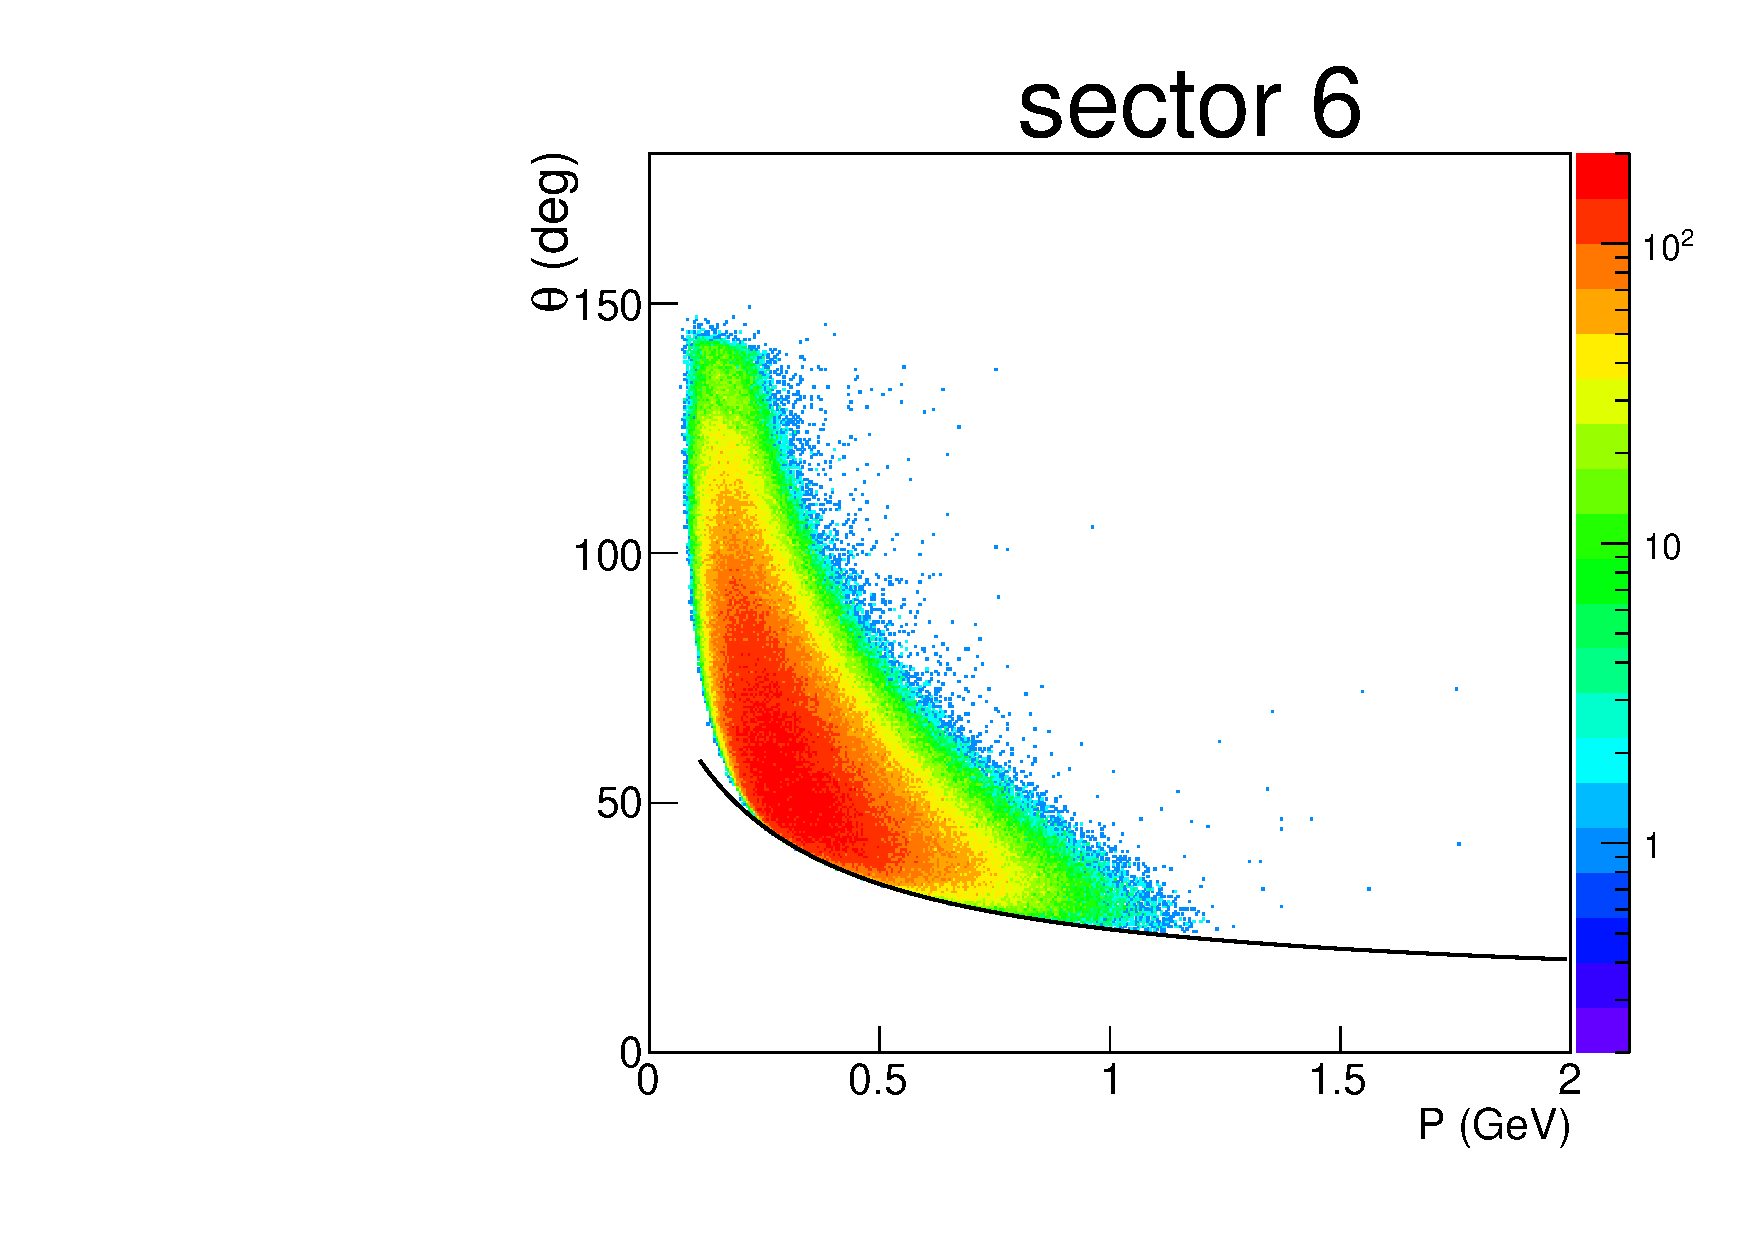
\includegraphics[width=5cm]{pictures/other_cuts/fiduch/th_vs_p_pim_sim/pim_th_vs_p_sim_sector6.pdf}
\end{framed}
\end{minipage}
%\end{framed}
\caption{\small $\theta$ versus momentum distributions for real $\pi^{-}$ events (upper frame)  and for Monte Carlo events (lower frame) for all six CLAS sectors. Black curves show cuts applied to remove inefficient areas. \label{fig:other_cuts_negaitive_th_vs_p_pions}}
\end{center}
\end{figure}

%\begin{figure}[htp]
%\begin{center}
%\begin{framed}
%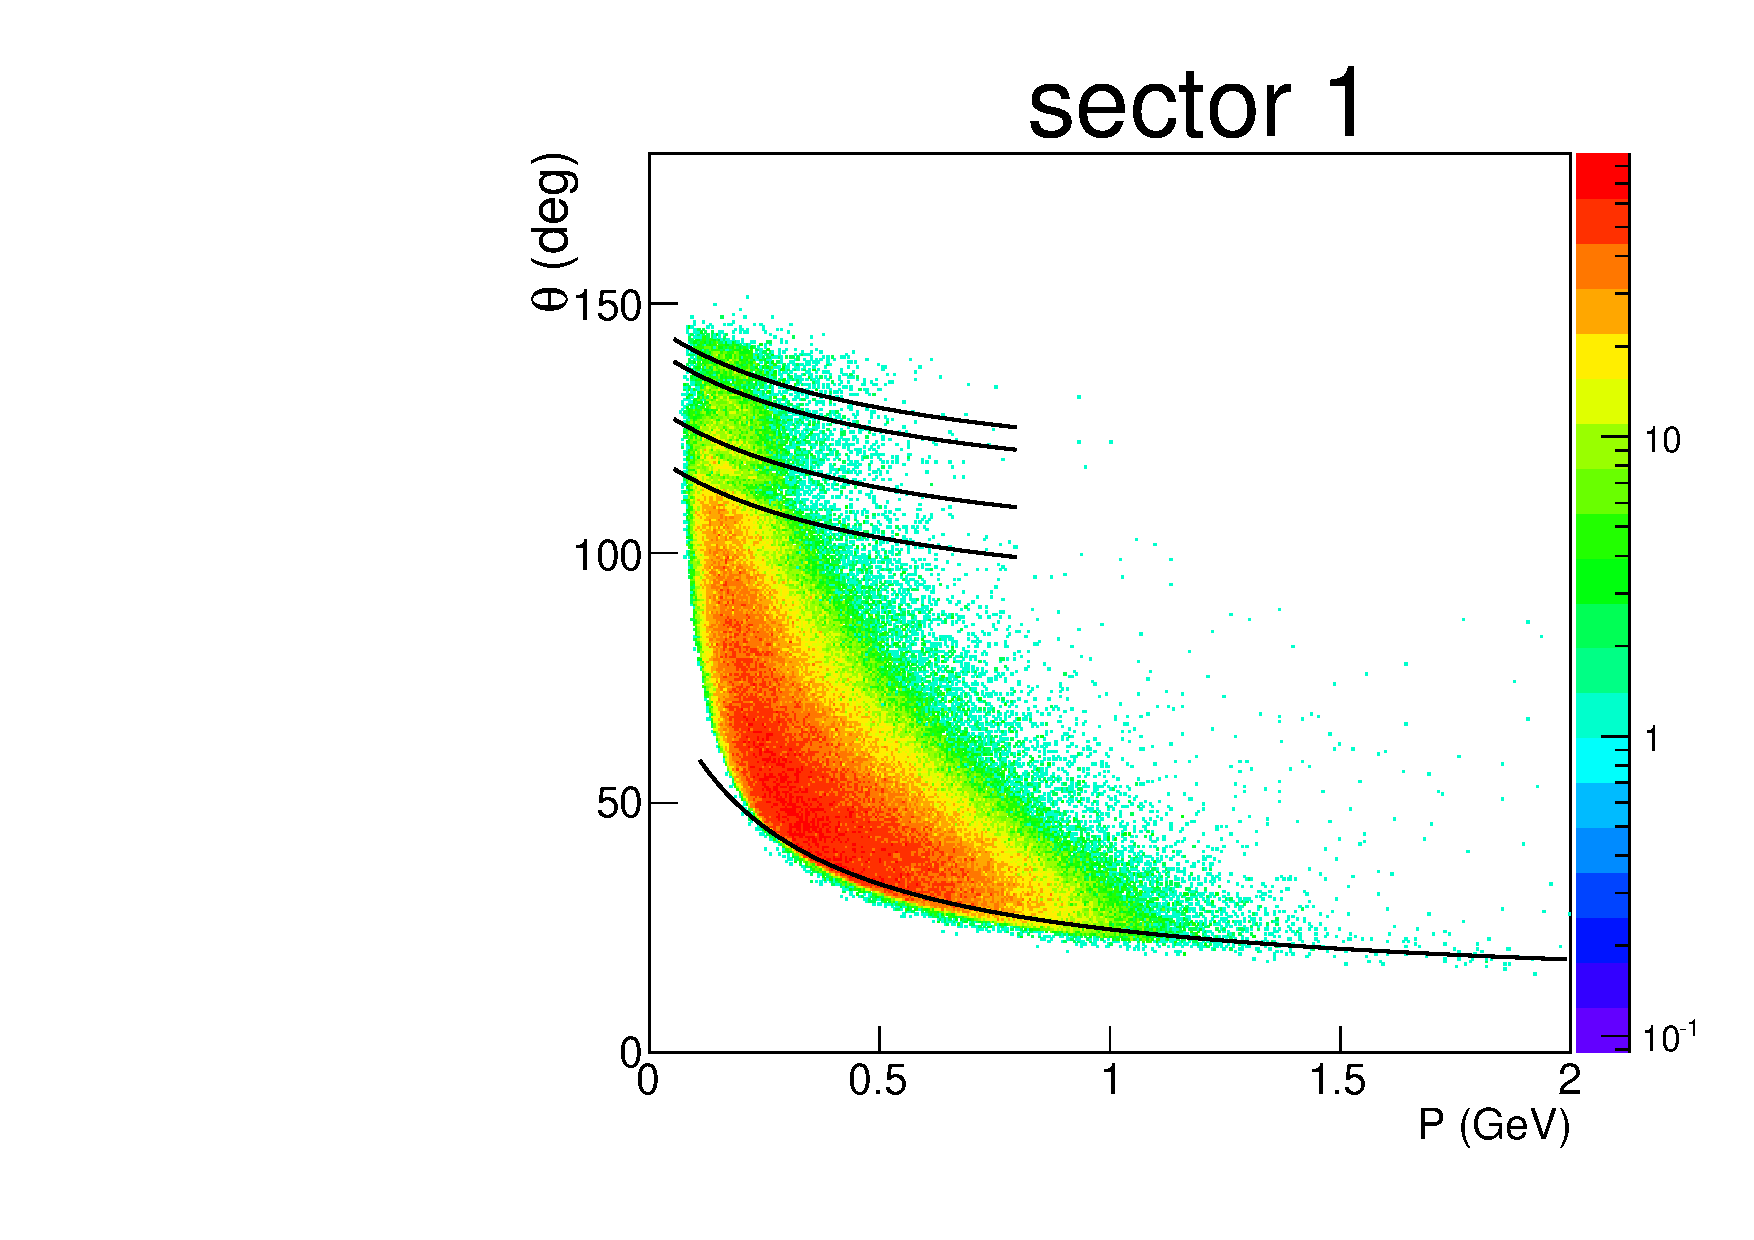
\includegraphics[width=5cm]{pictures/other_cuts/fiduch/th_vs_p_pim/pim_th_vs_p_sector1.pdf}
%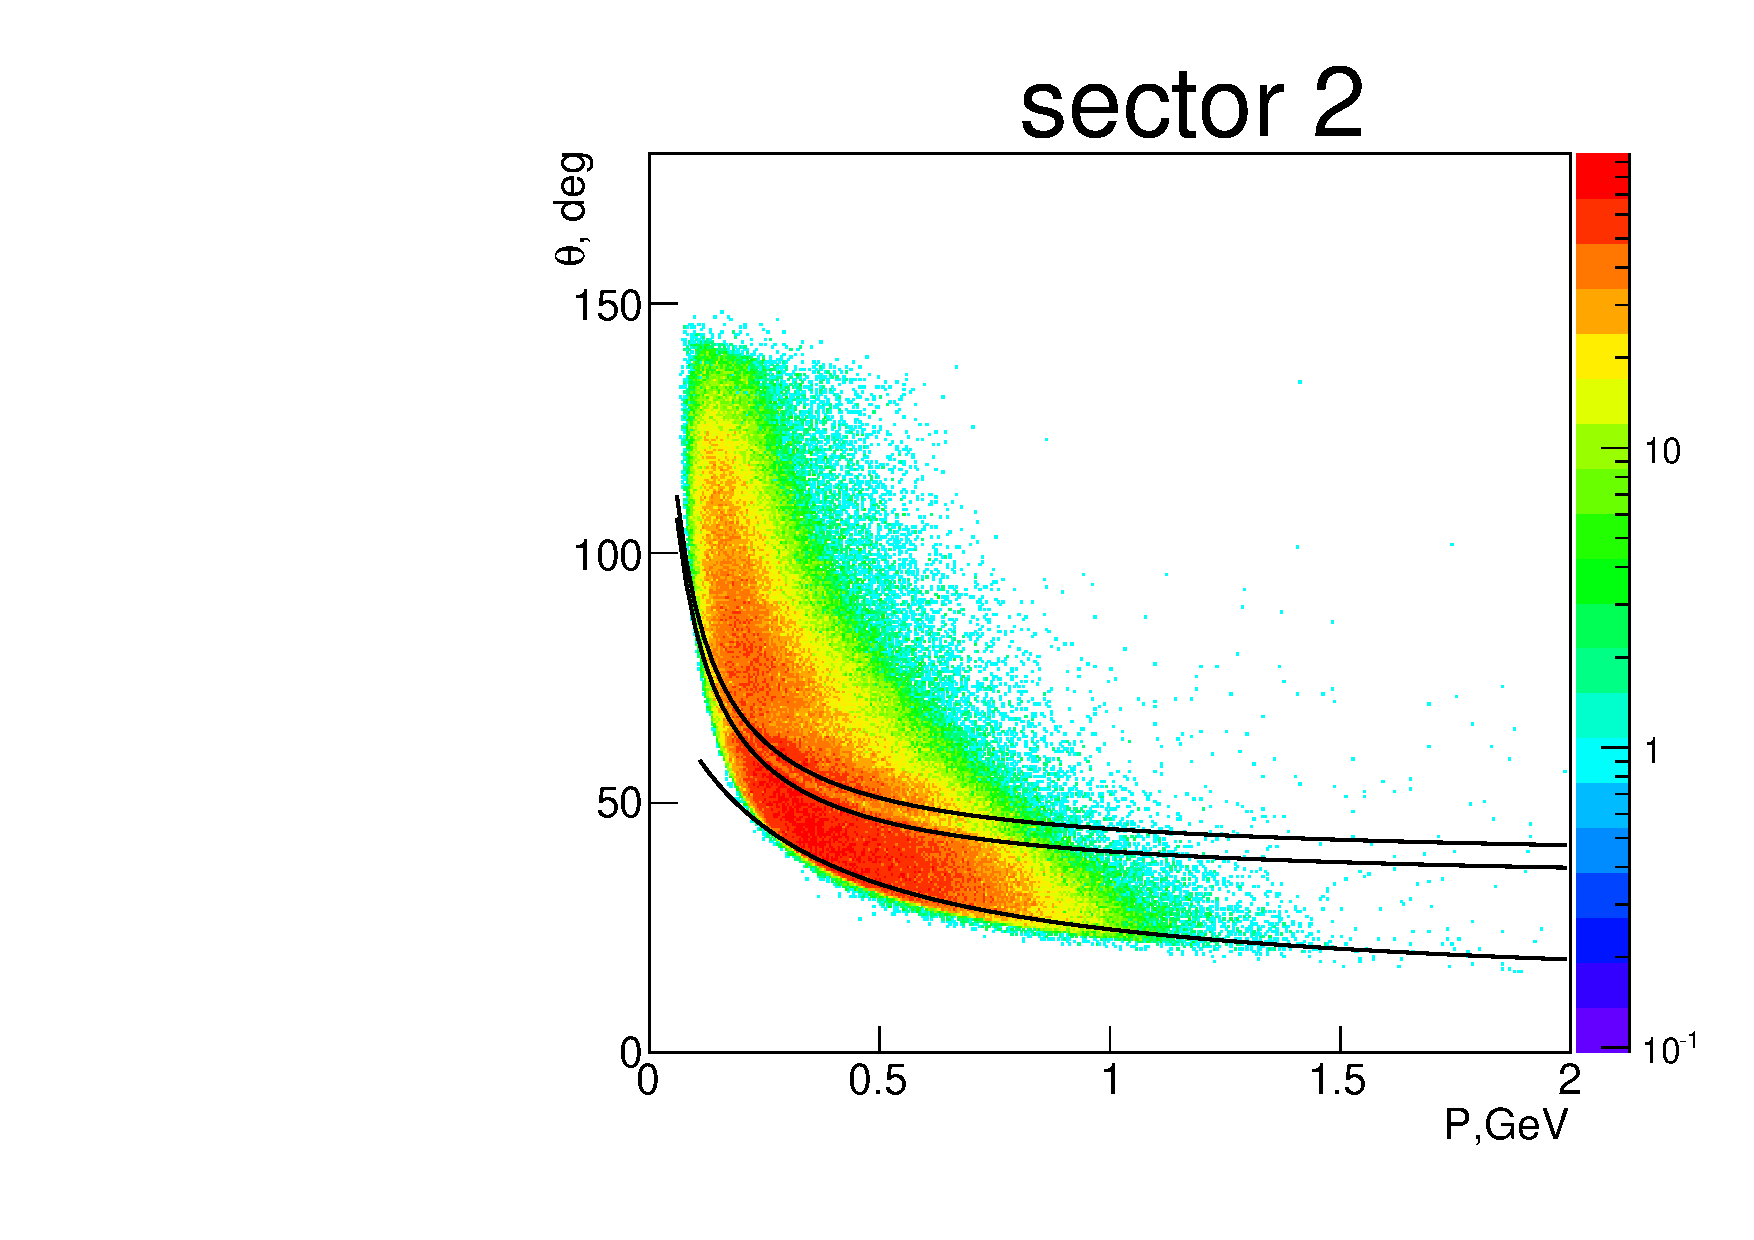
\includegraphics[width=5cm]{pictures/other_cuts/fiduch/th_vs_p_pim/pim_th_vs_p_sector2.pdf}
%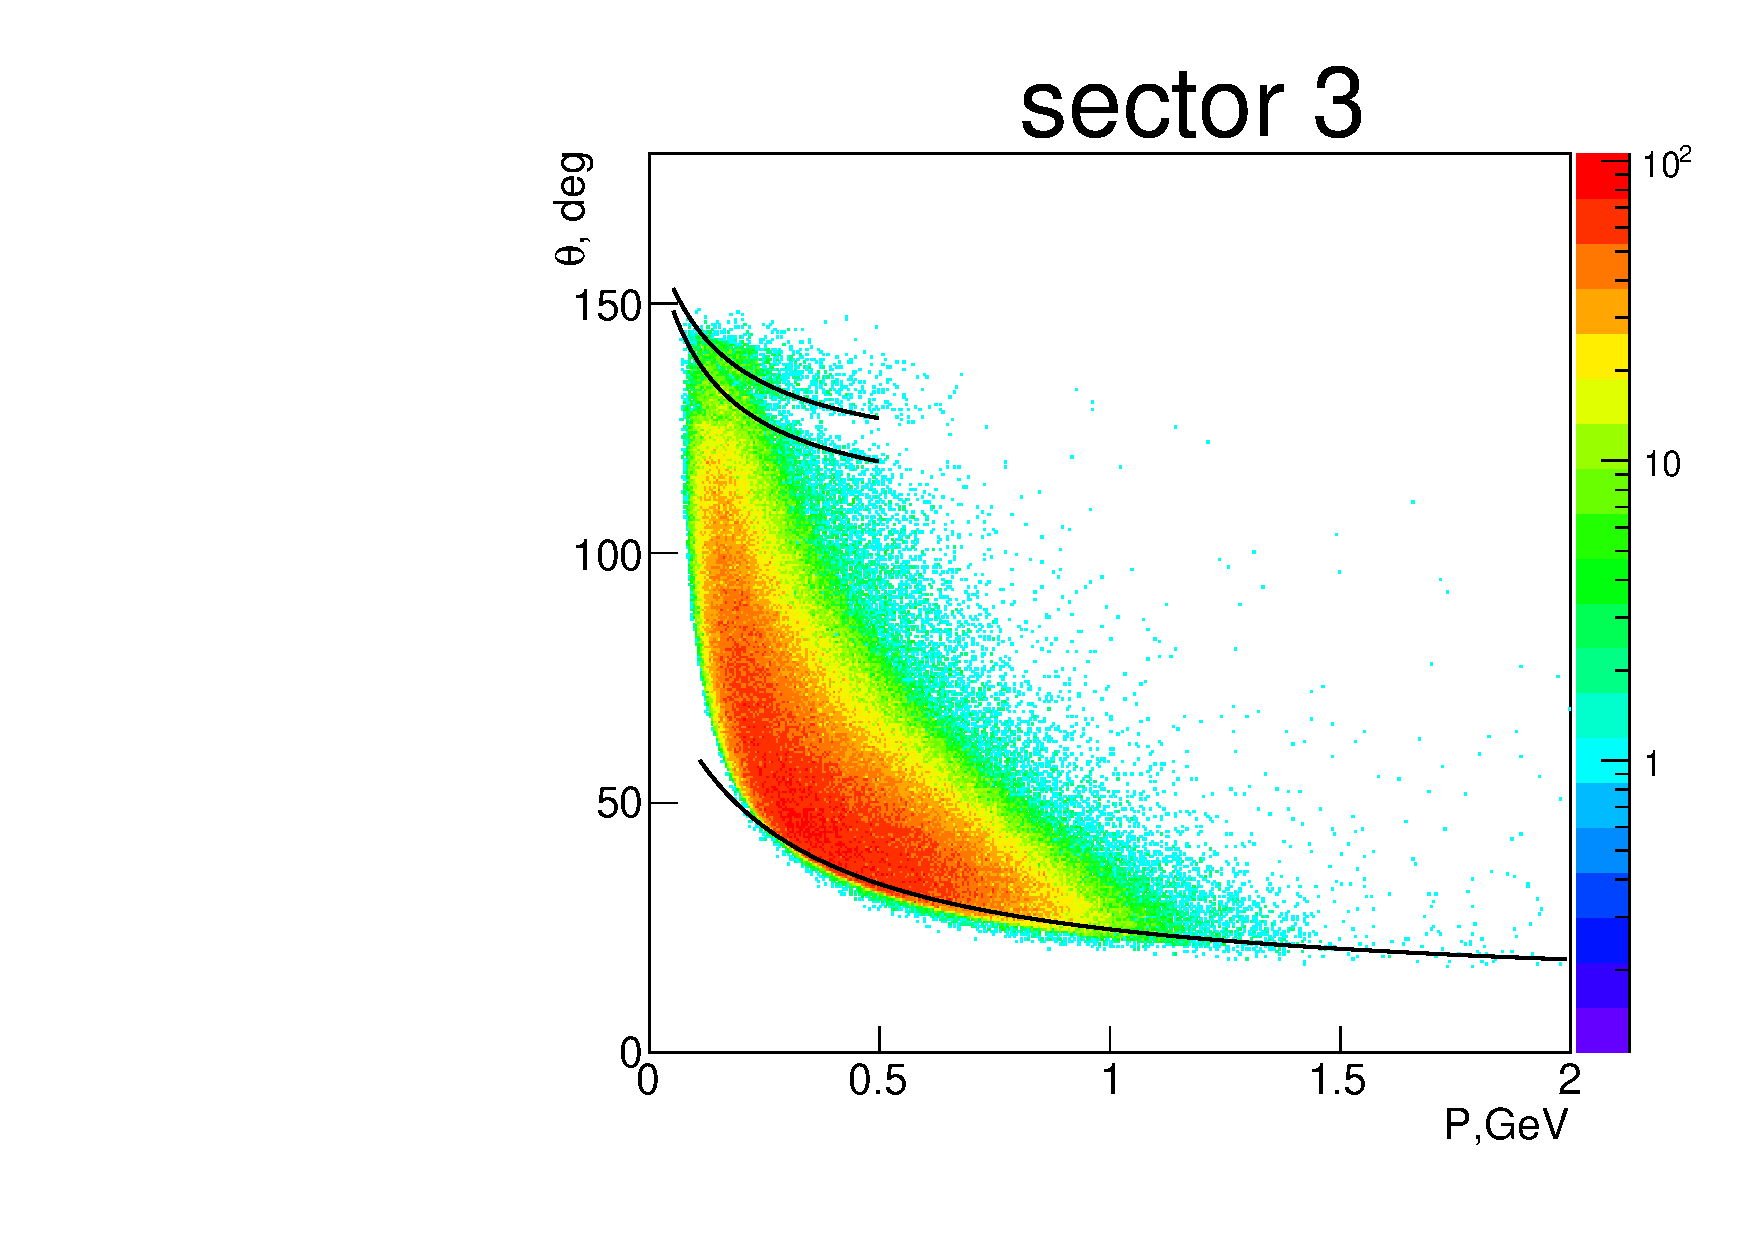
\includegraphics[width=5cm]{pictures/other_cuts/fiduch/th_vs_p_pim/pim_th_vs_p_sector3.pdf}
%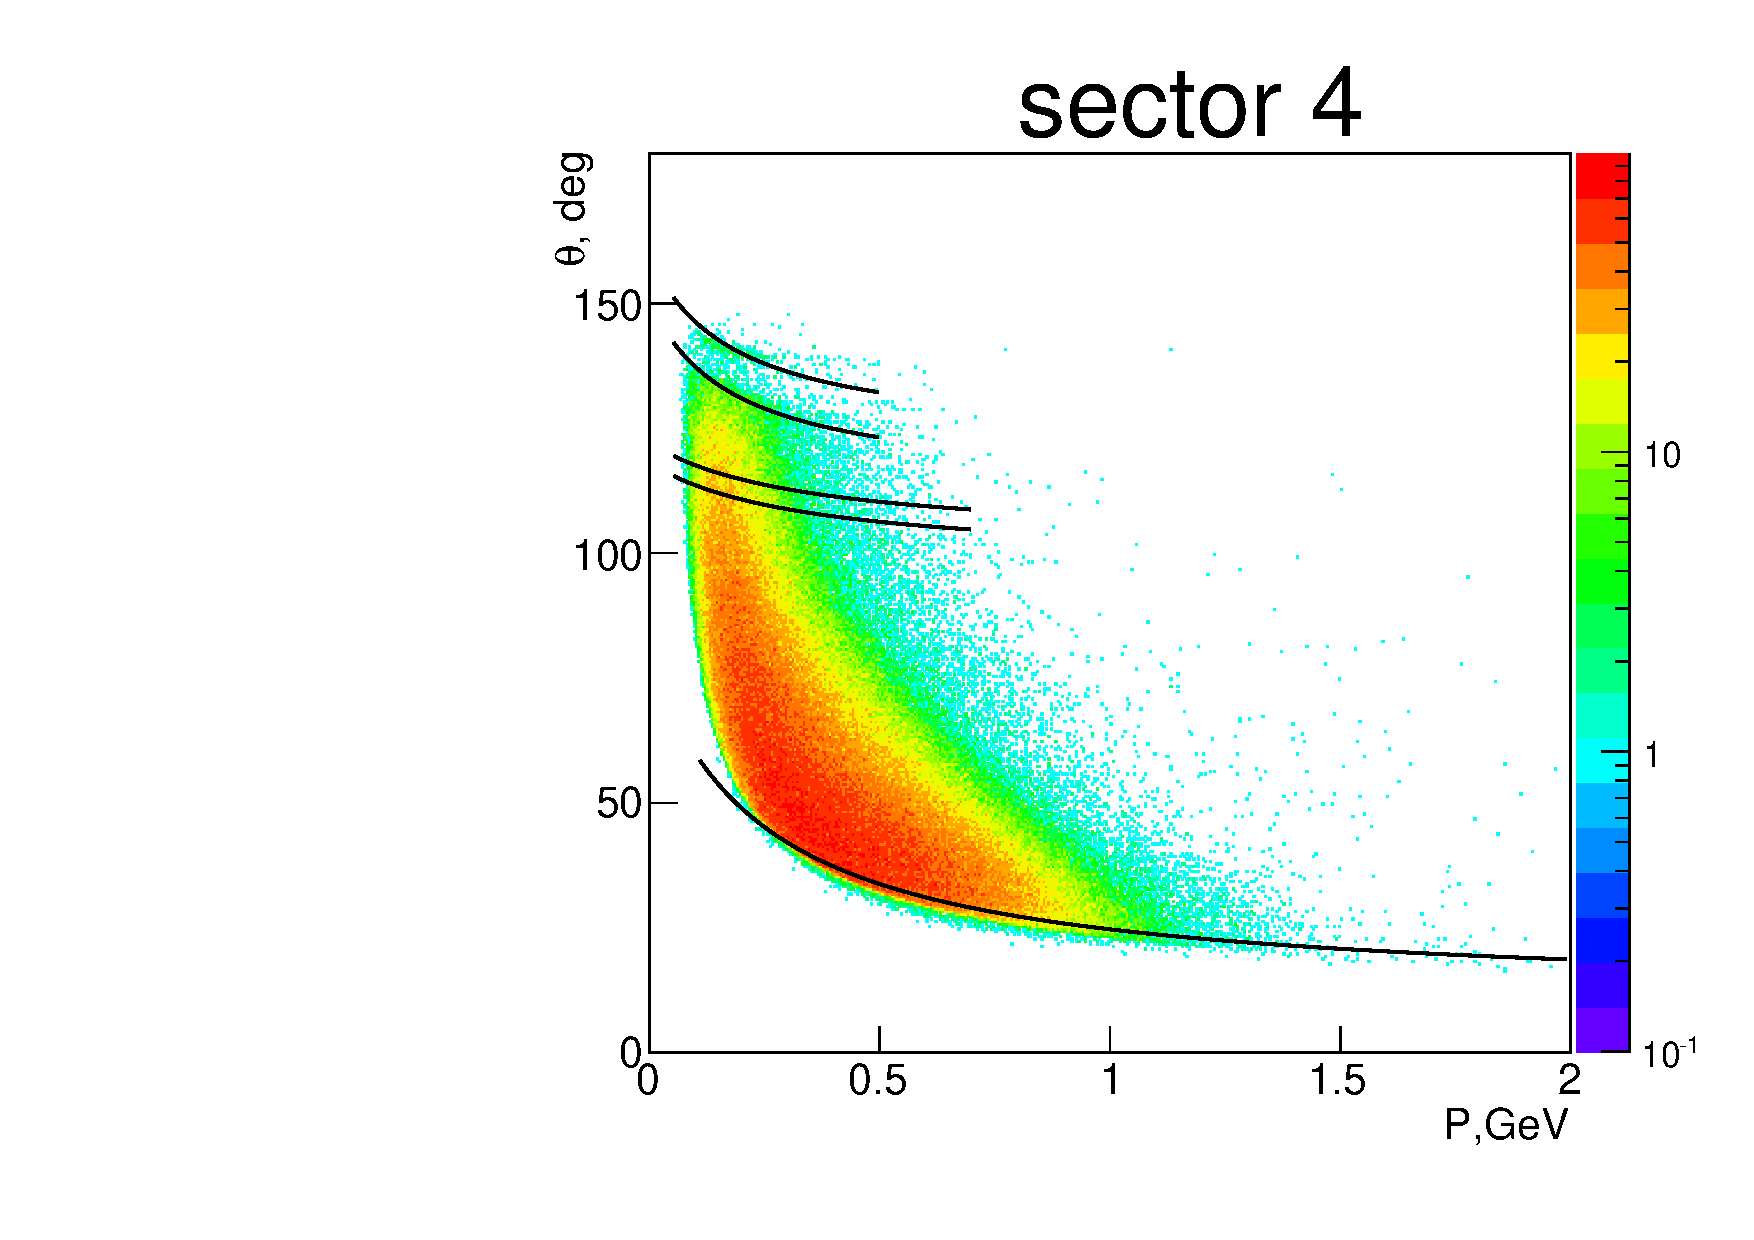
\includegraphics[width=5cm]{pictures/other_cuts/fiduch/th_vs_p_pim/pim_th_vs_p_sector4.pdf}
%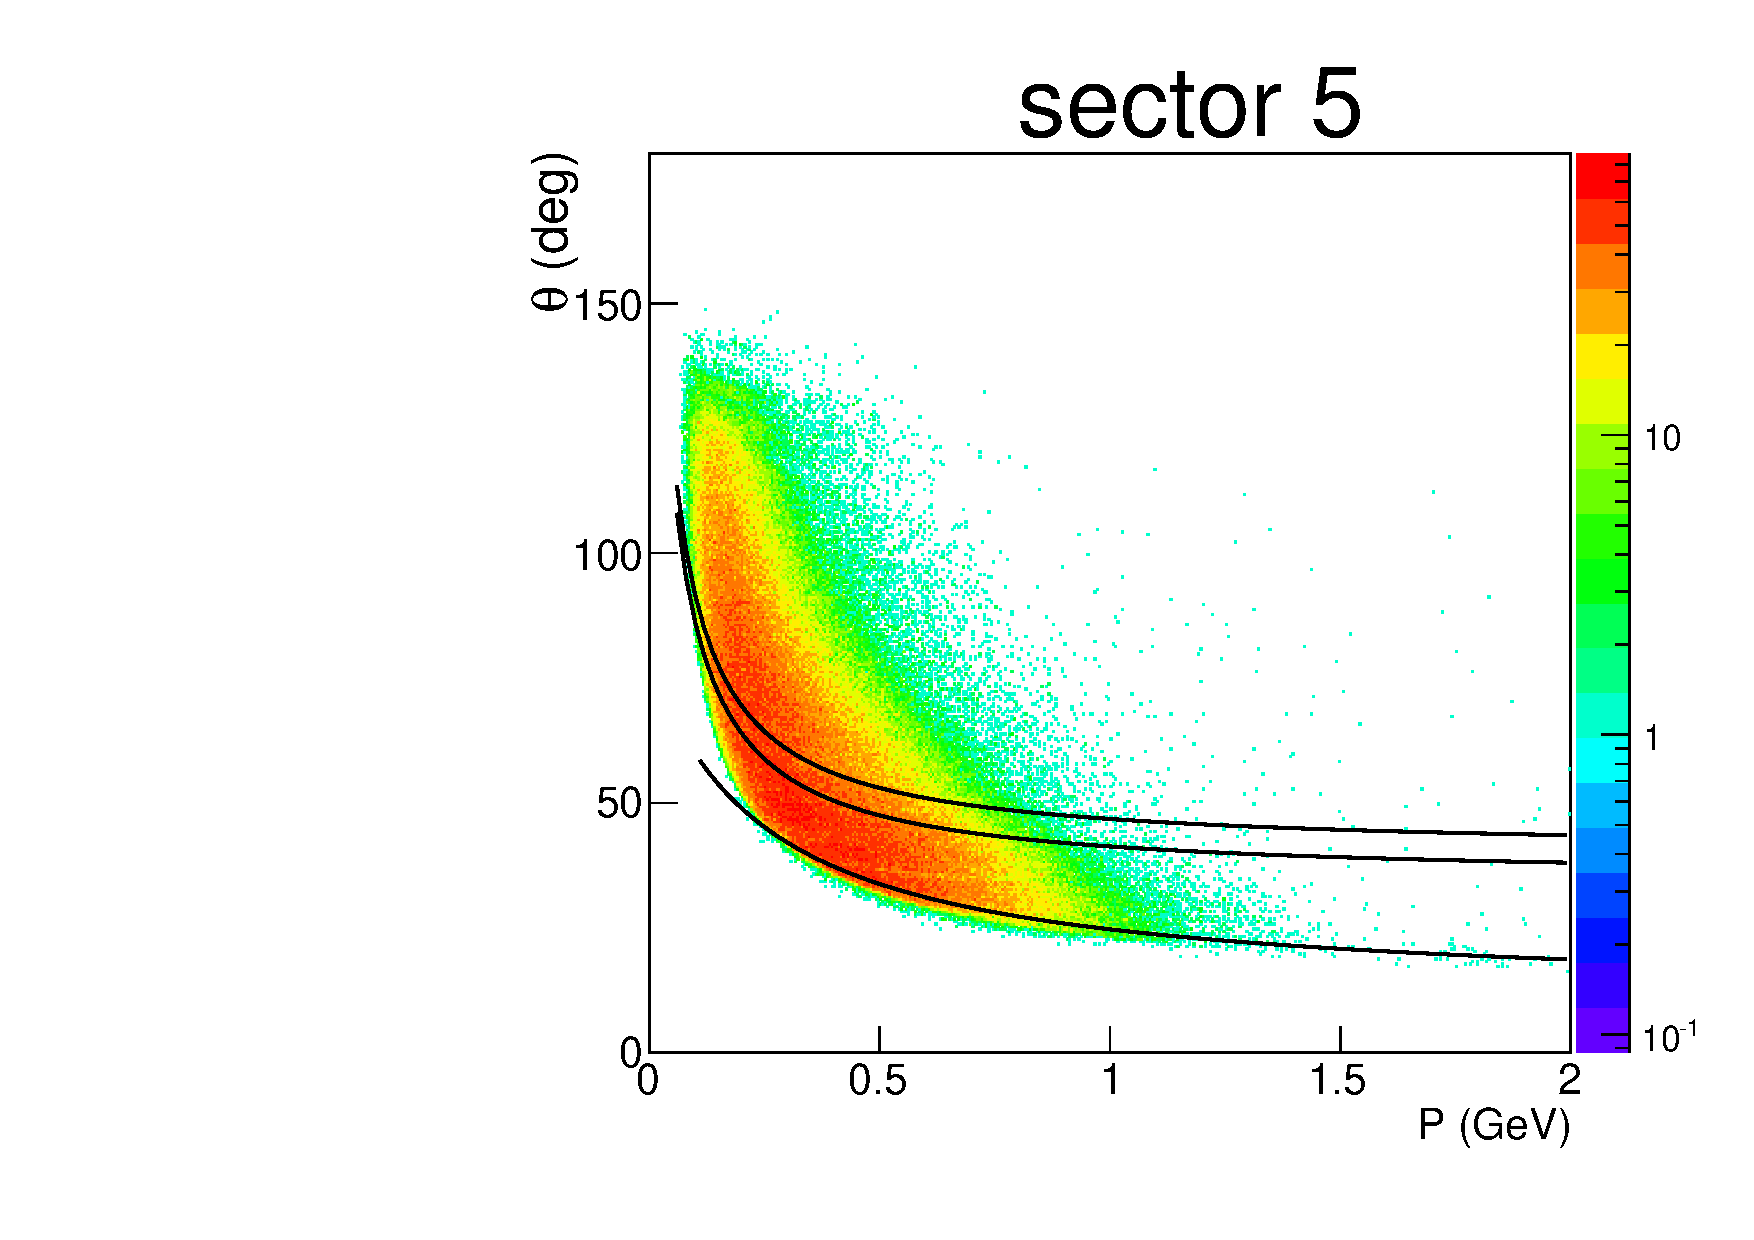
\includegraphics[width=5cm]{pictures/other_cuts/fiduch/th_vs_p_pim/pim_th_vs_p_sector5.pdf}
%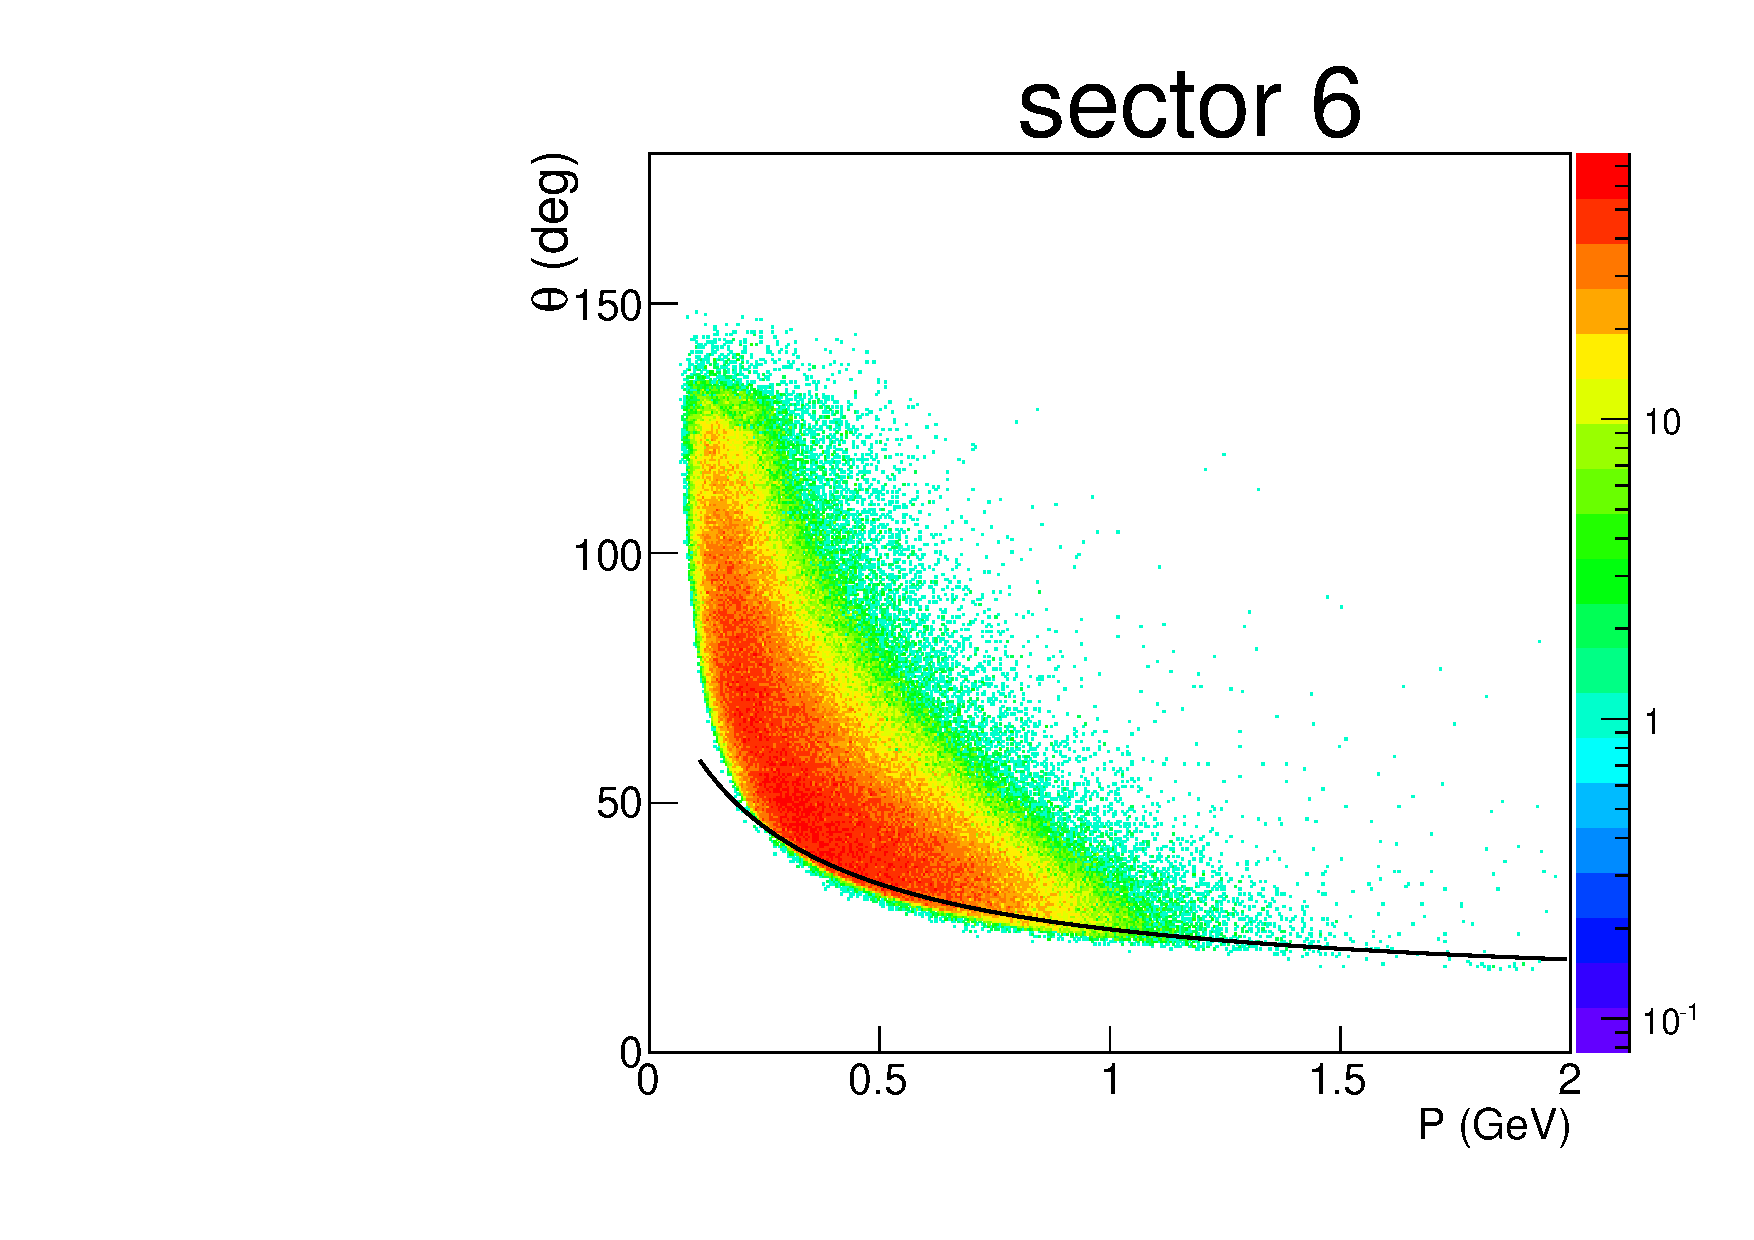
\includegraphics[width=5cm]{pictures/other_cuts/fiduch/th_vs_p_pim/pim_th_vs_p_sector6.pdf}
%\end{framed}
%\caption{\small $\theta$ versus momentum distributions for $\pi^{-}$ . \label{fig:eother_cuts_pim_th_vs_p}}
%\end{center}
%\end{figure}
\subsection{Fiducial cuts for positively charged particles}
\label{fiduch_positive}
For positively charged particles, which are outbending in the e1e experiment, momentum independent and asymmetrical fiducial cuts are the best choice. These cuts are established in the same way as for negatively charged particles, i.e.
by selection of the flat parts of the event distributions over $\varphi$.
The shape of these cuts is given by

\begin{equation}
\begin{aligned}
\varphi_{upper} & =  24(1-e^{-0.08(\theta-9)}) \\
\varphi_{lower} & = -25(1-e^{-0.1(\theta-10)}),   
\label{eq:fiduch_positive}
\end{aligned}  
\end{equation}
where $\theta$ is the particle angle in degrees. $\varphi_{upper}$ and $\varphi_{lower}$ are the upper and lower cut boundaries. Events with $\varphi_{lower} < \varphi < \varphi_{upper}$ are selected for further analysis. 

This function is superimposed on the 2D $\varphi$ versus $\theta$ distributions of real events and shown in Fig.~\ref{fig:eother_cuts_positive_fiduch_2d} by the black curves.
Additional cuts in $\theta$ versus momentum coordinates are shown by the black curves for Monte Carlo and real events in Fig.~\ref{fig:other_cuts_positive_th_vs_p_protons} for protons and in Fig.~\ref{fig:other_cuts_positive_th_vs_p_piplus} for $\pi^{+}$.





\begin{figure}[htp]
\begin{center}
\begin{minipage}{.49\textwidth}
\framebox{
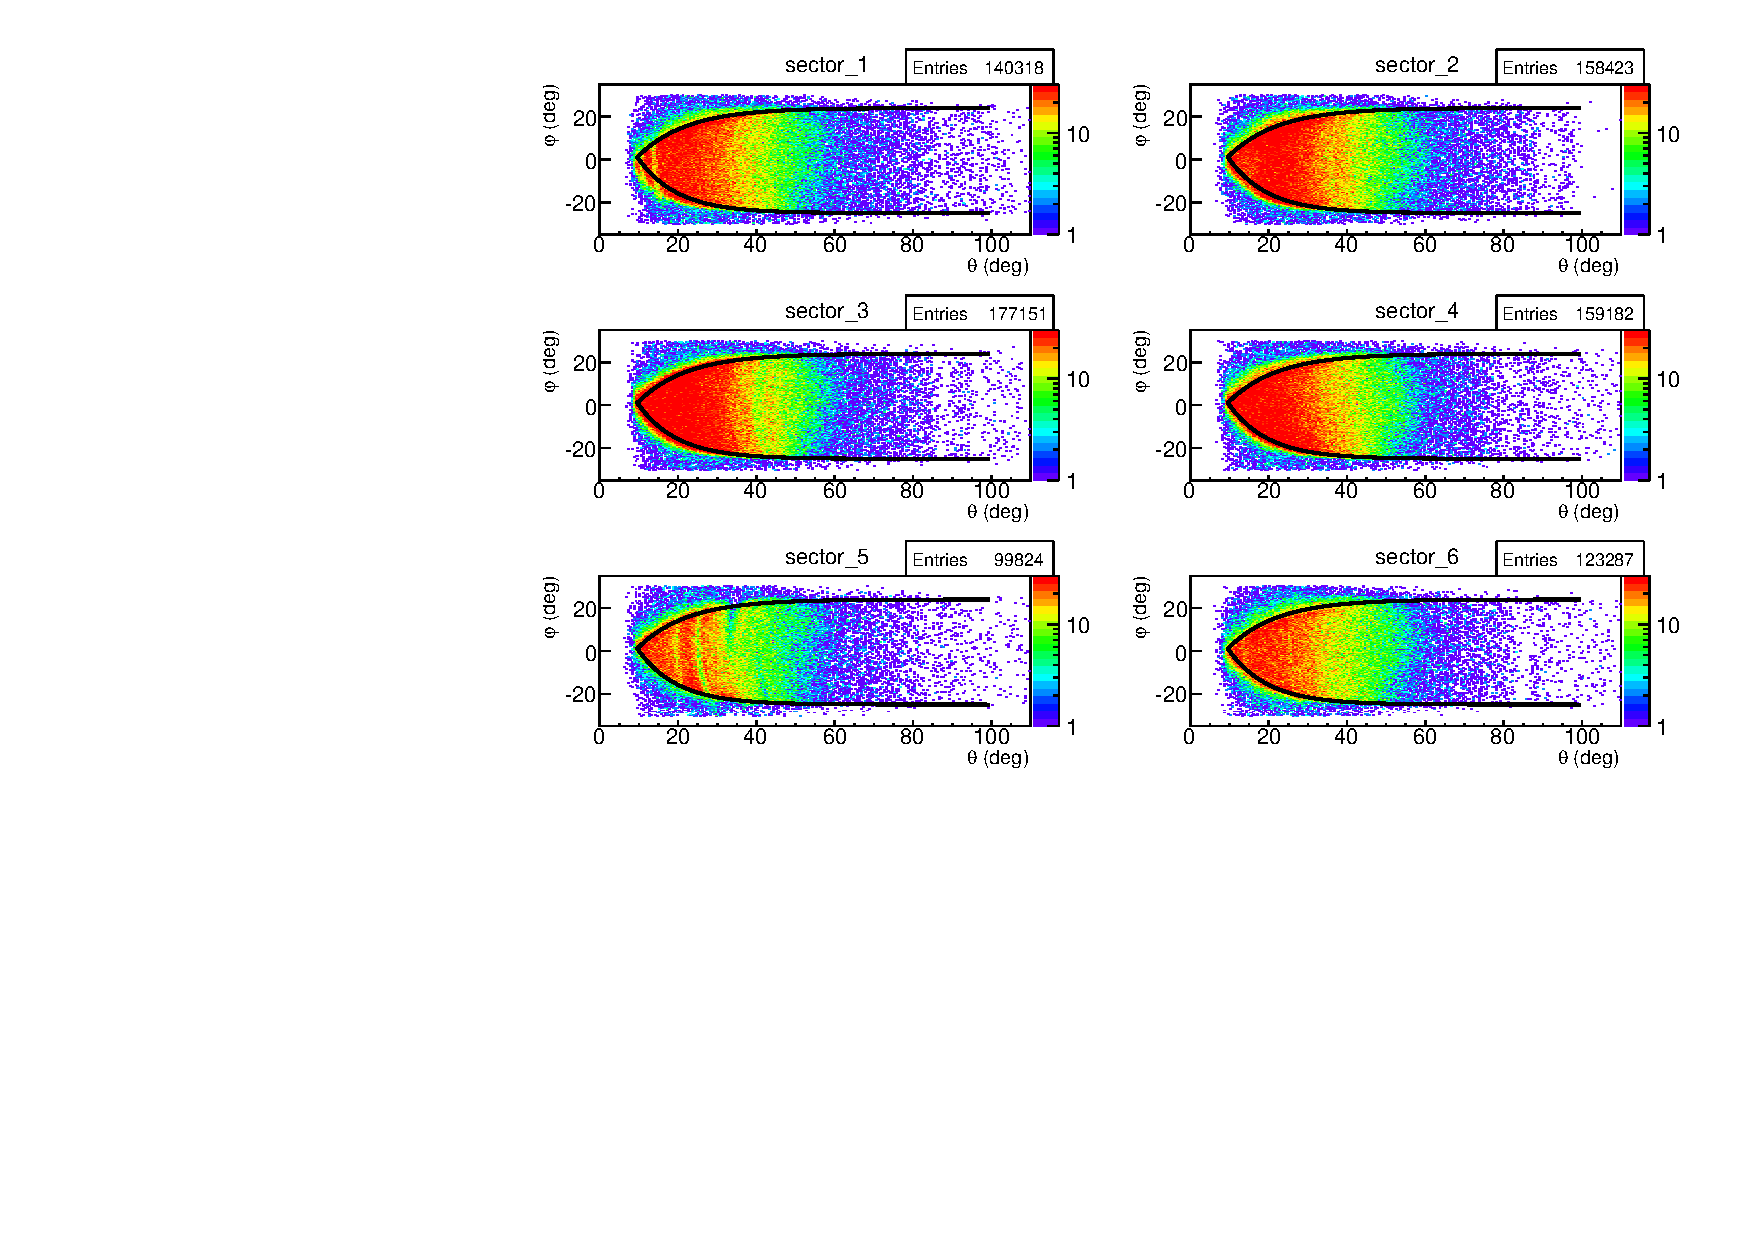
\includegraphics[width=7.6cm]{pictures/other_cuts/fiduch/p_fid_2dim_2.pdf}
}
\end{minipage}
\begin{minipage}{.49\textwidth}
\framebox{
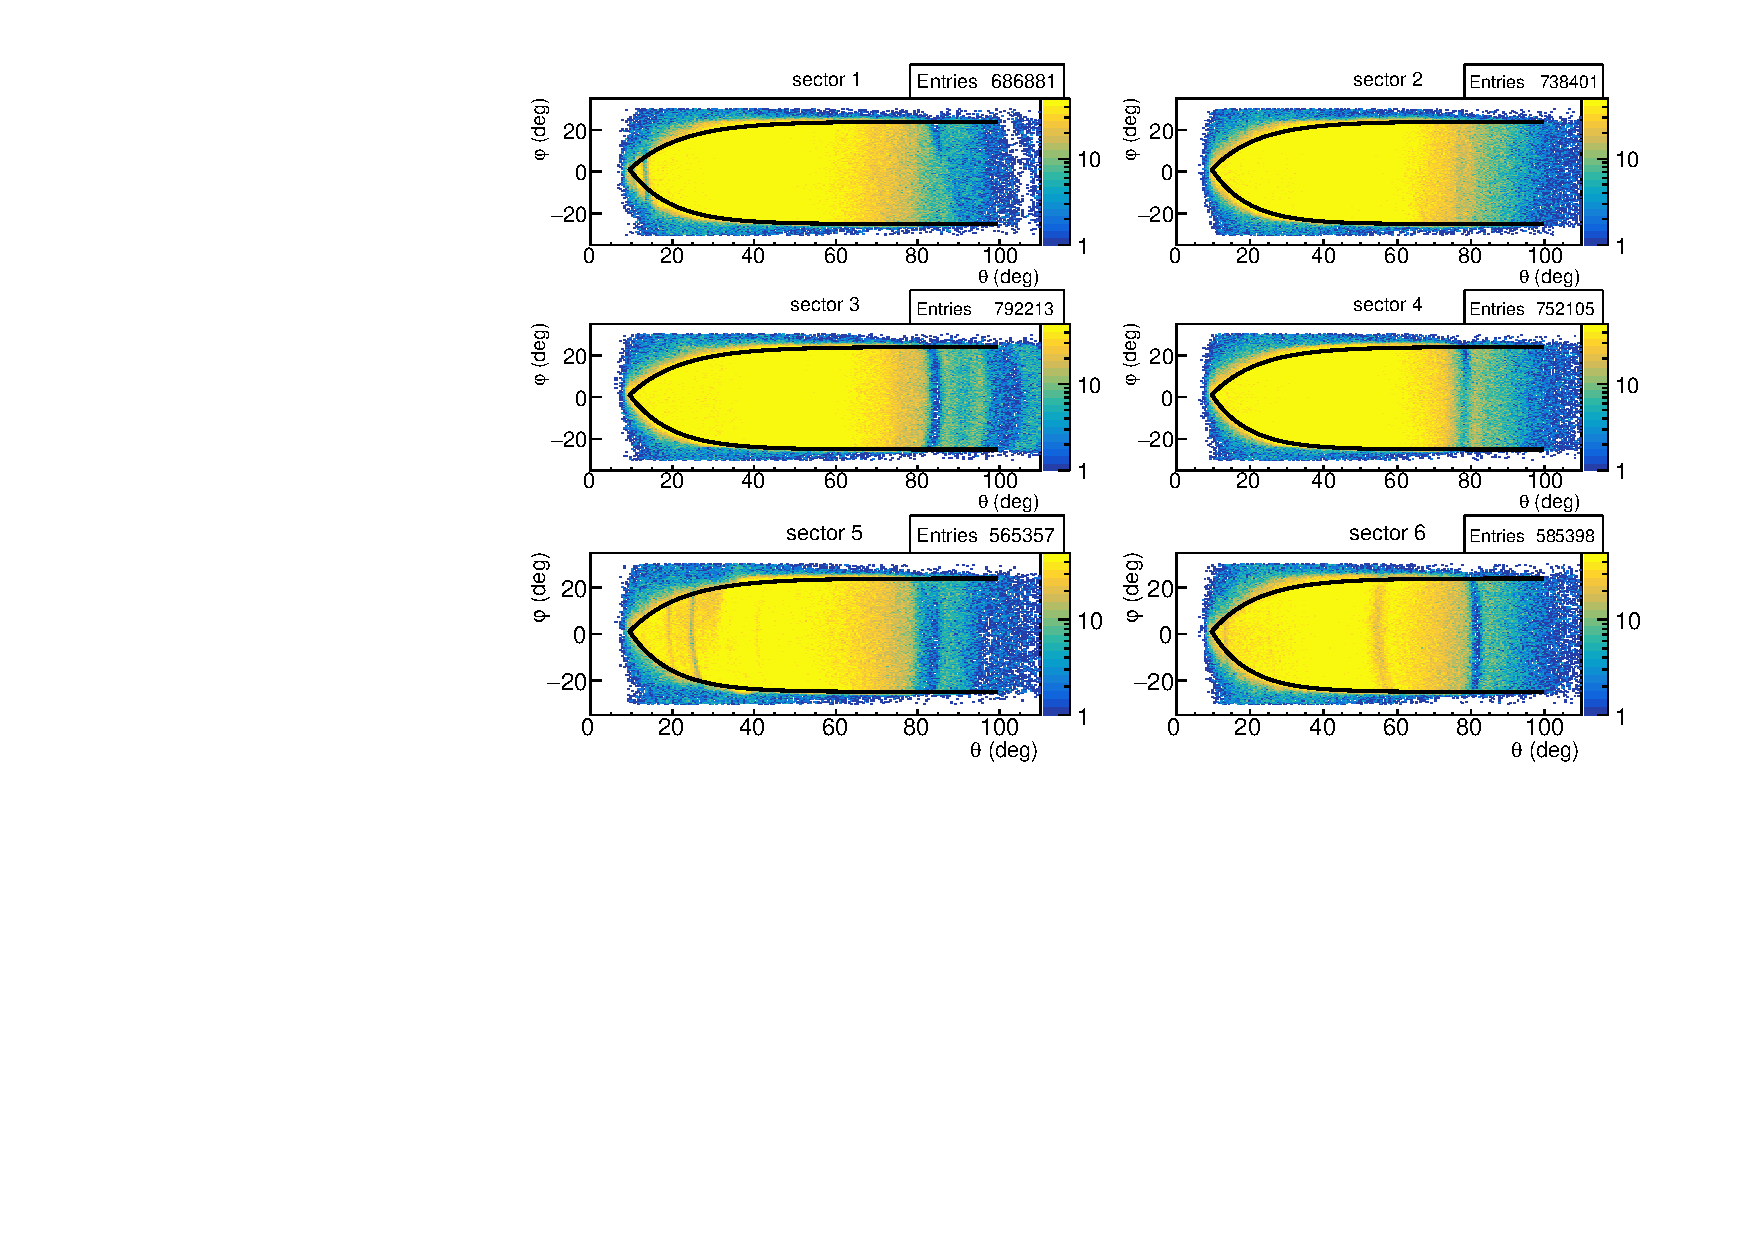
\includegraphics[width=7.6cm]{pictures/other_cuts/fiduch/pip_fid_2dim_2.pdf}
}
\end{minipage}
\caption{\small $\varphi$ versus $\theta$ distributions for protons with momenta from 600 MeV to 800 MeV (left frame) and $\pi^{+}$ with momenta from 400 MeV to 600 MeV (right frame) for all six CLAS sectors. Curves show the applied fiducial cuts. \label{fig:eother_cuts_positive_fiduch_2d}}
\end{center}
\end{figure}




\begin{figure}[htp]
\begin{center}
%\begin{framed}
\begin{minipage}{.99\textwidth}
\begin{framed}
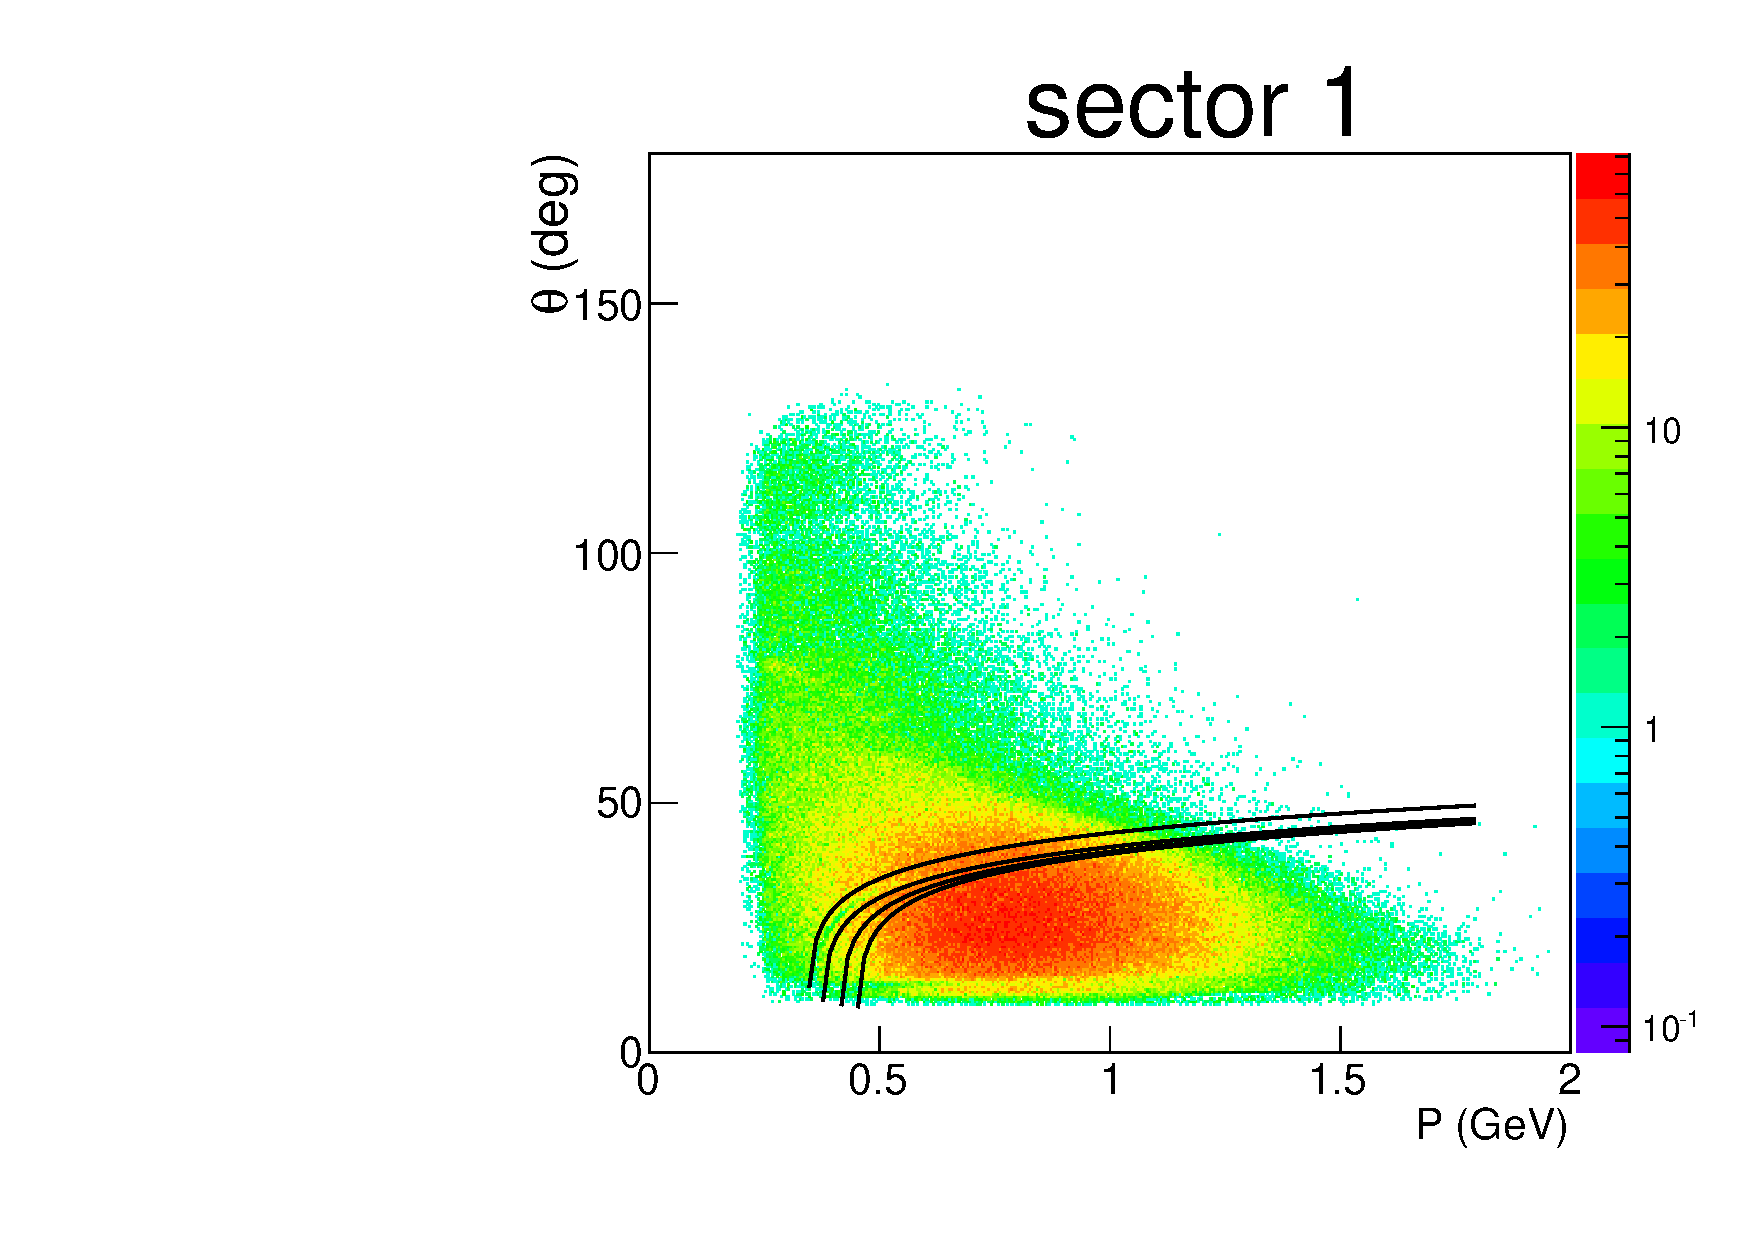
\includegraphics[width=5cm]{pictures/other_cuts/fiduch/th_vs_p_p/p_th_vs_p_sector1.pdf}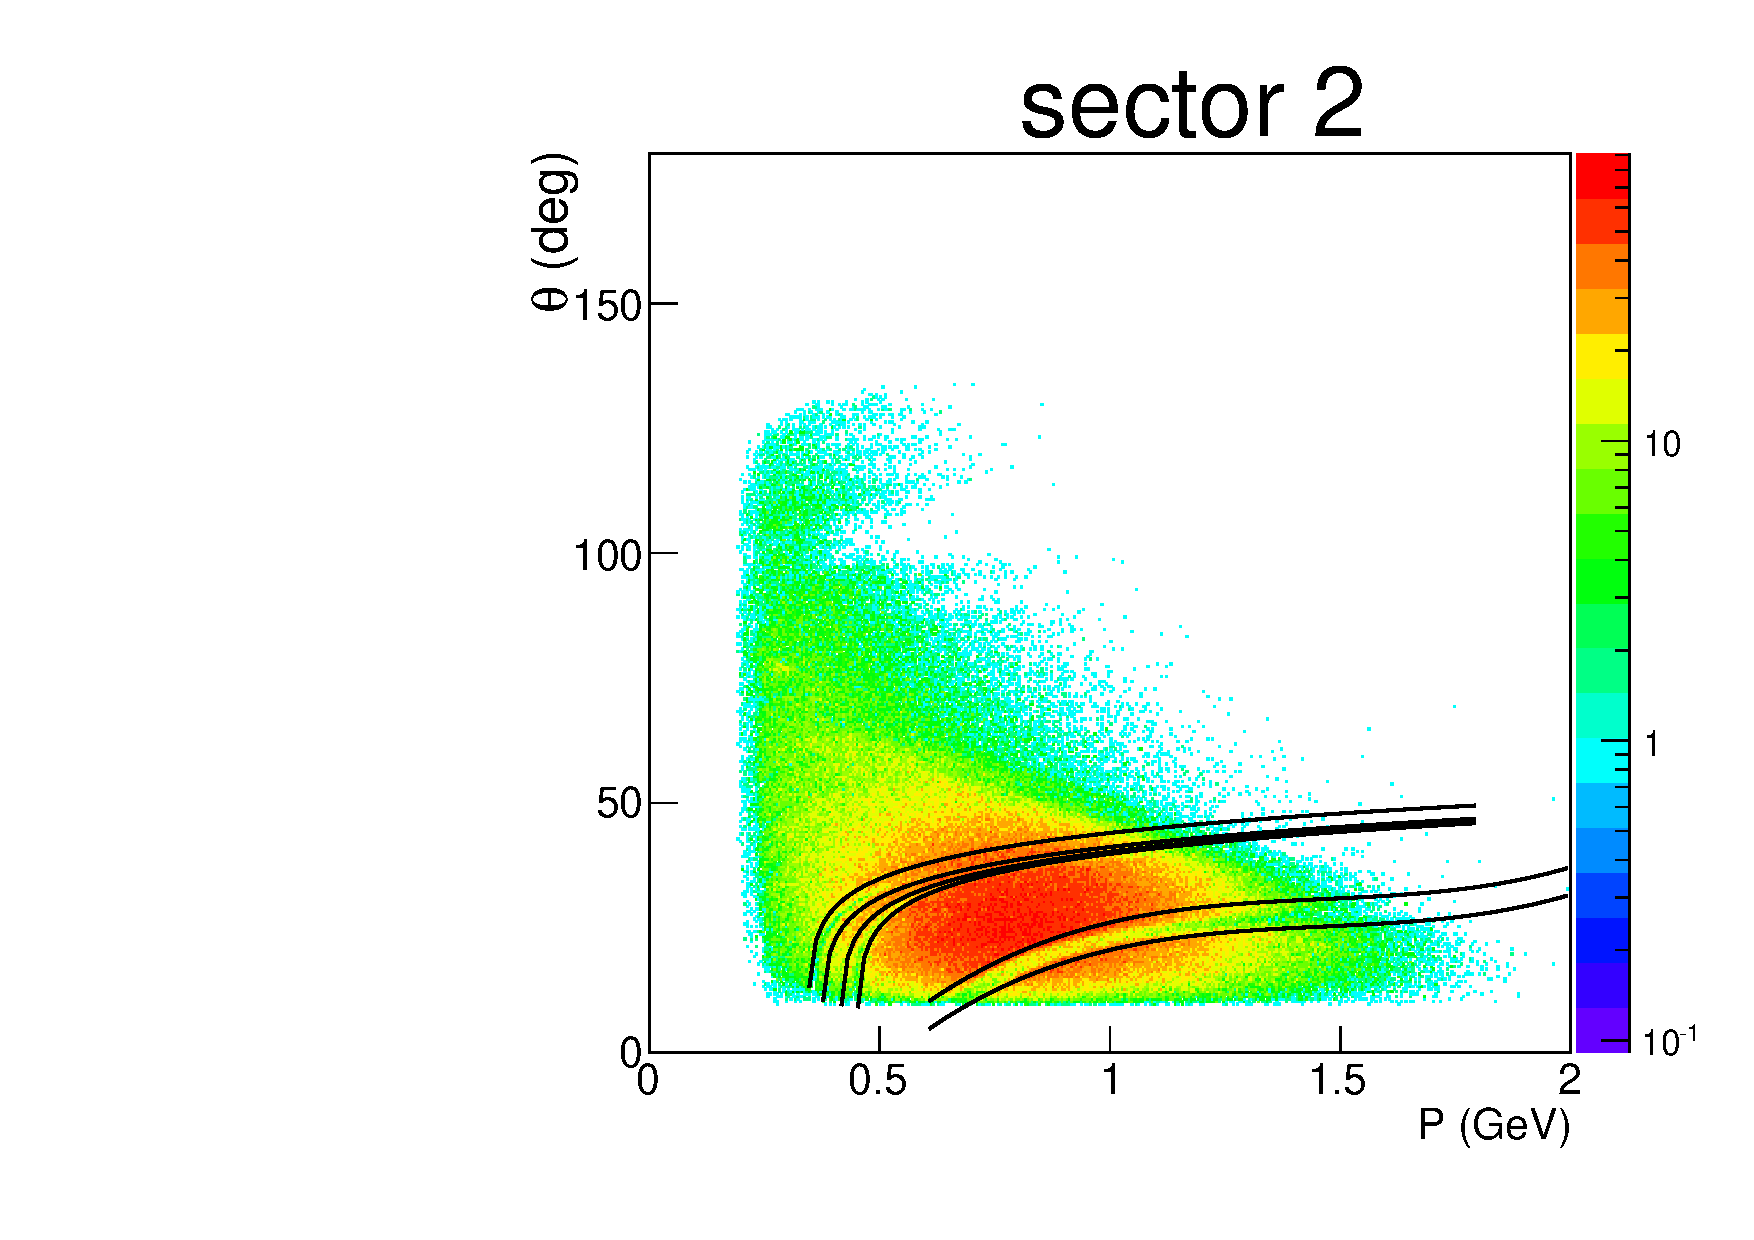
\includegraphics[width=5cm]{pictures/other_cuts/fiduch/th_vs_p_p/p_th_vs_p_sector2.pdf}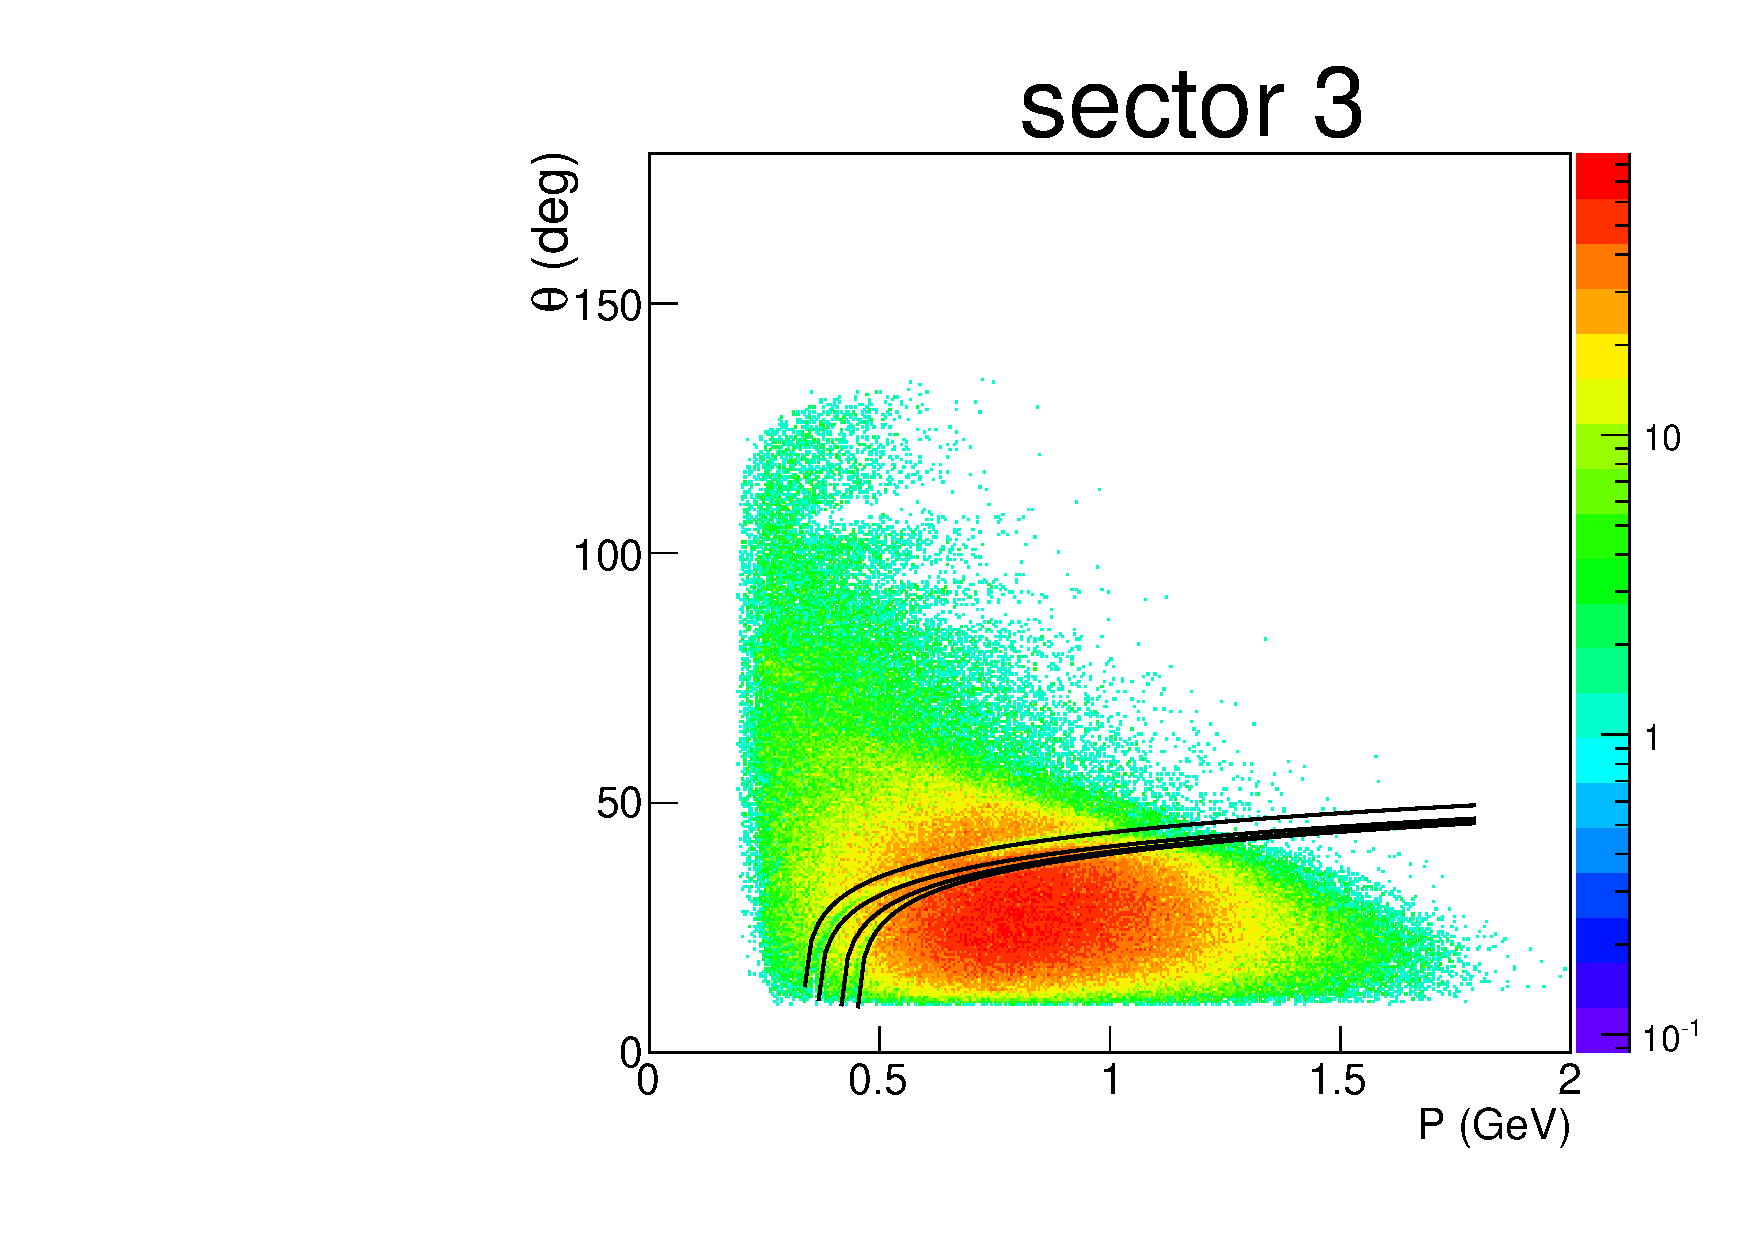
\includegraphics[width=5cm]{pictures/other_cuts/fiduch/th_vs_p_p/p_th_vs_p_sector3.pdf}
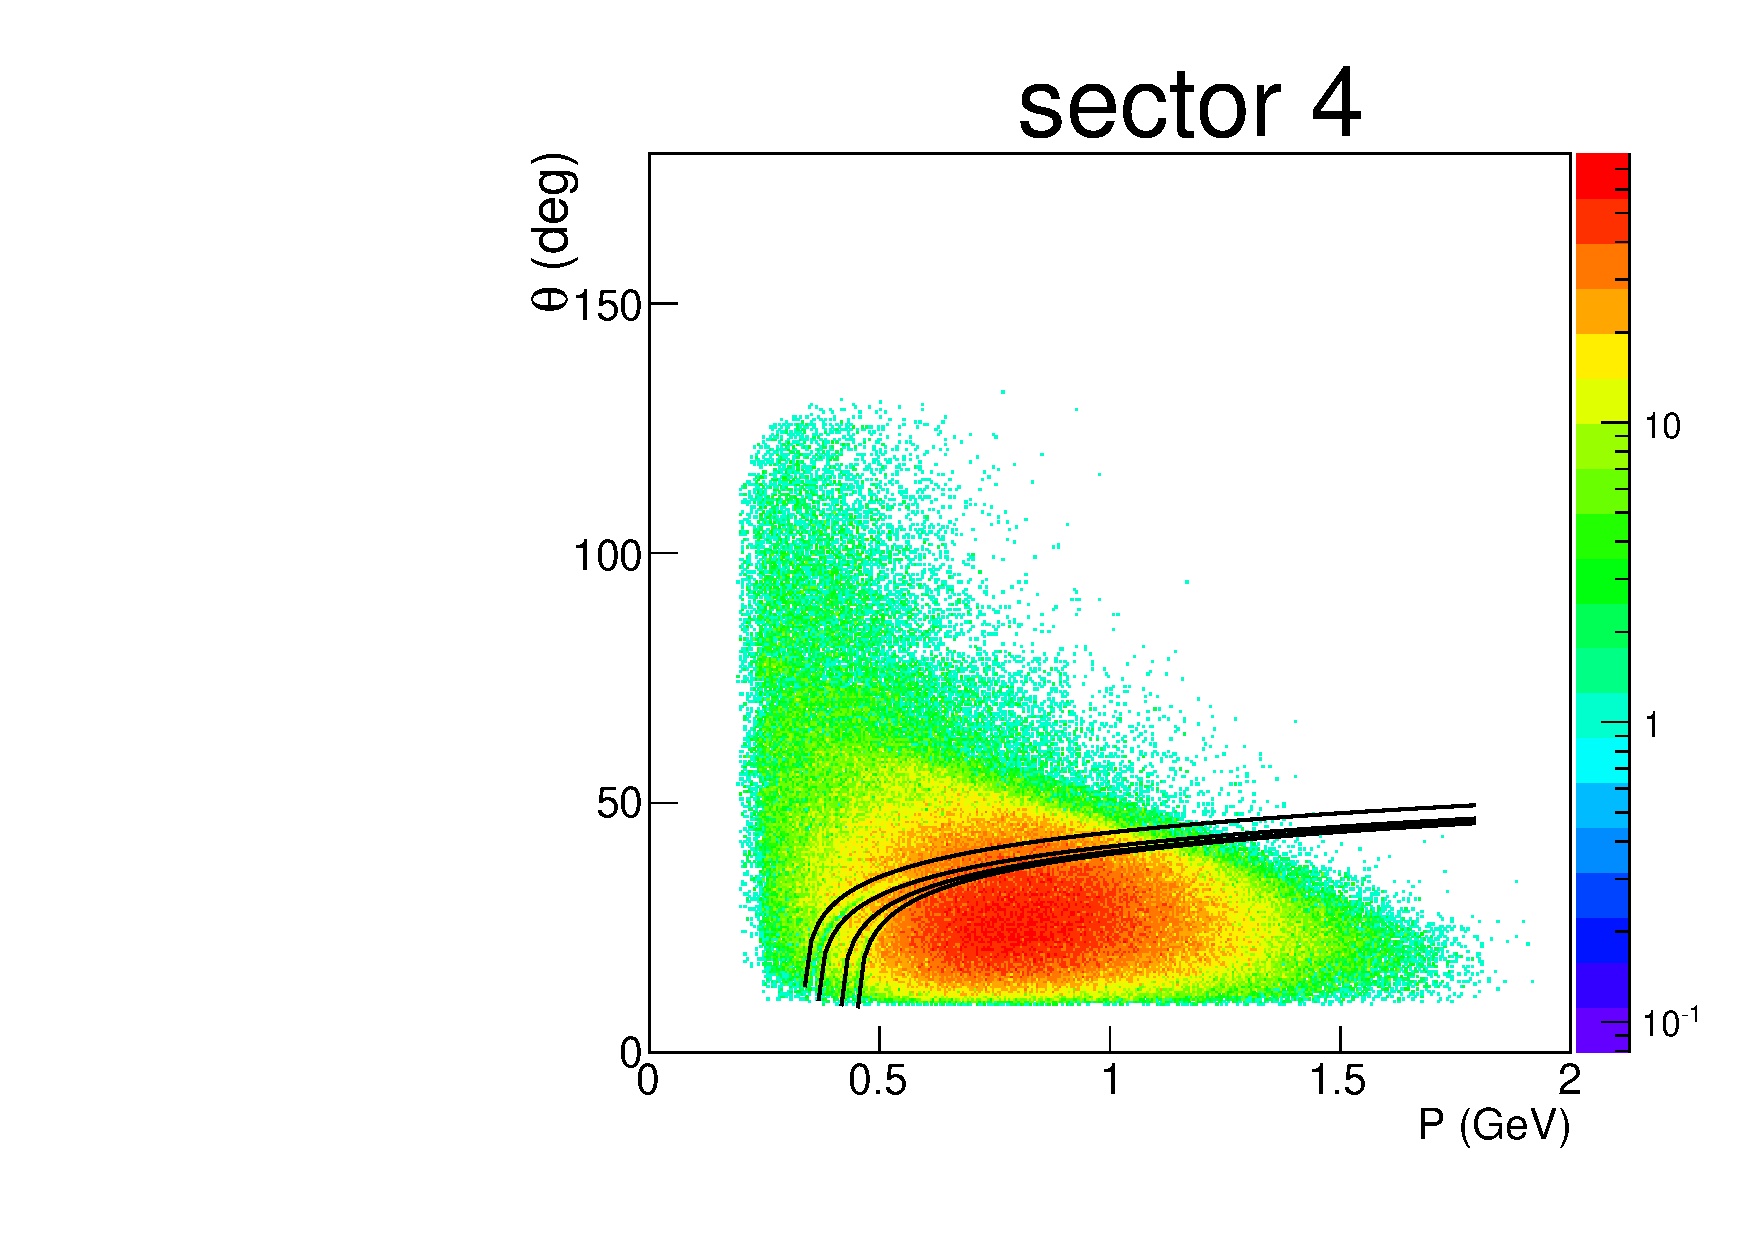
\includegraphics[width=5cm]{pictures/other_cuts/fiduch/th_vs_p_p/p_th_vs_p_sector4.pdf}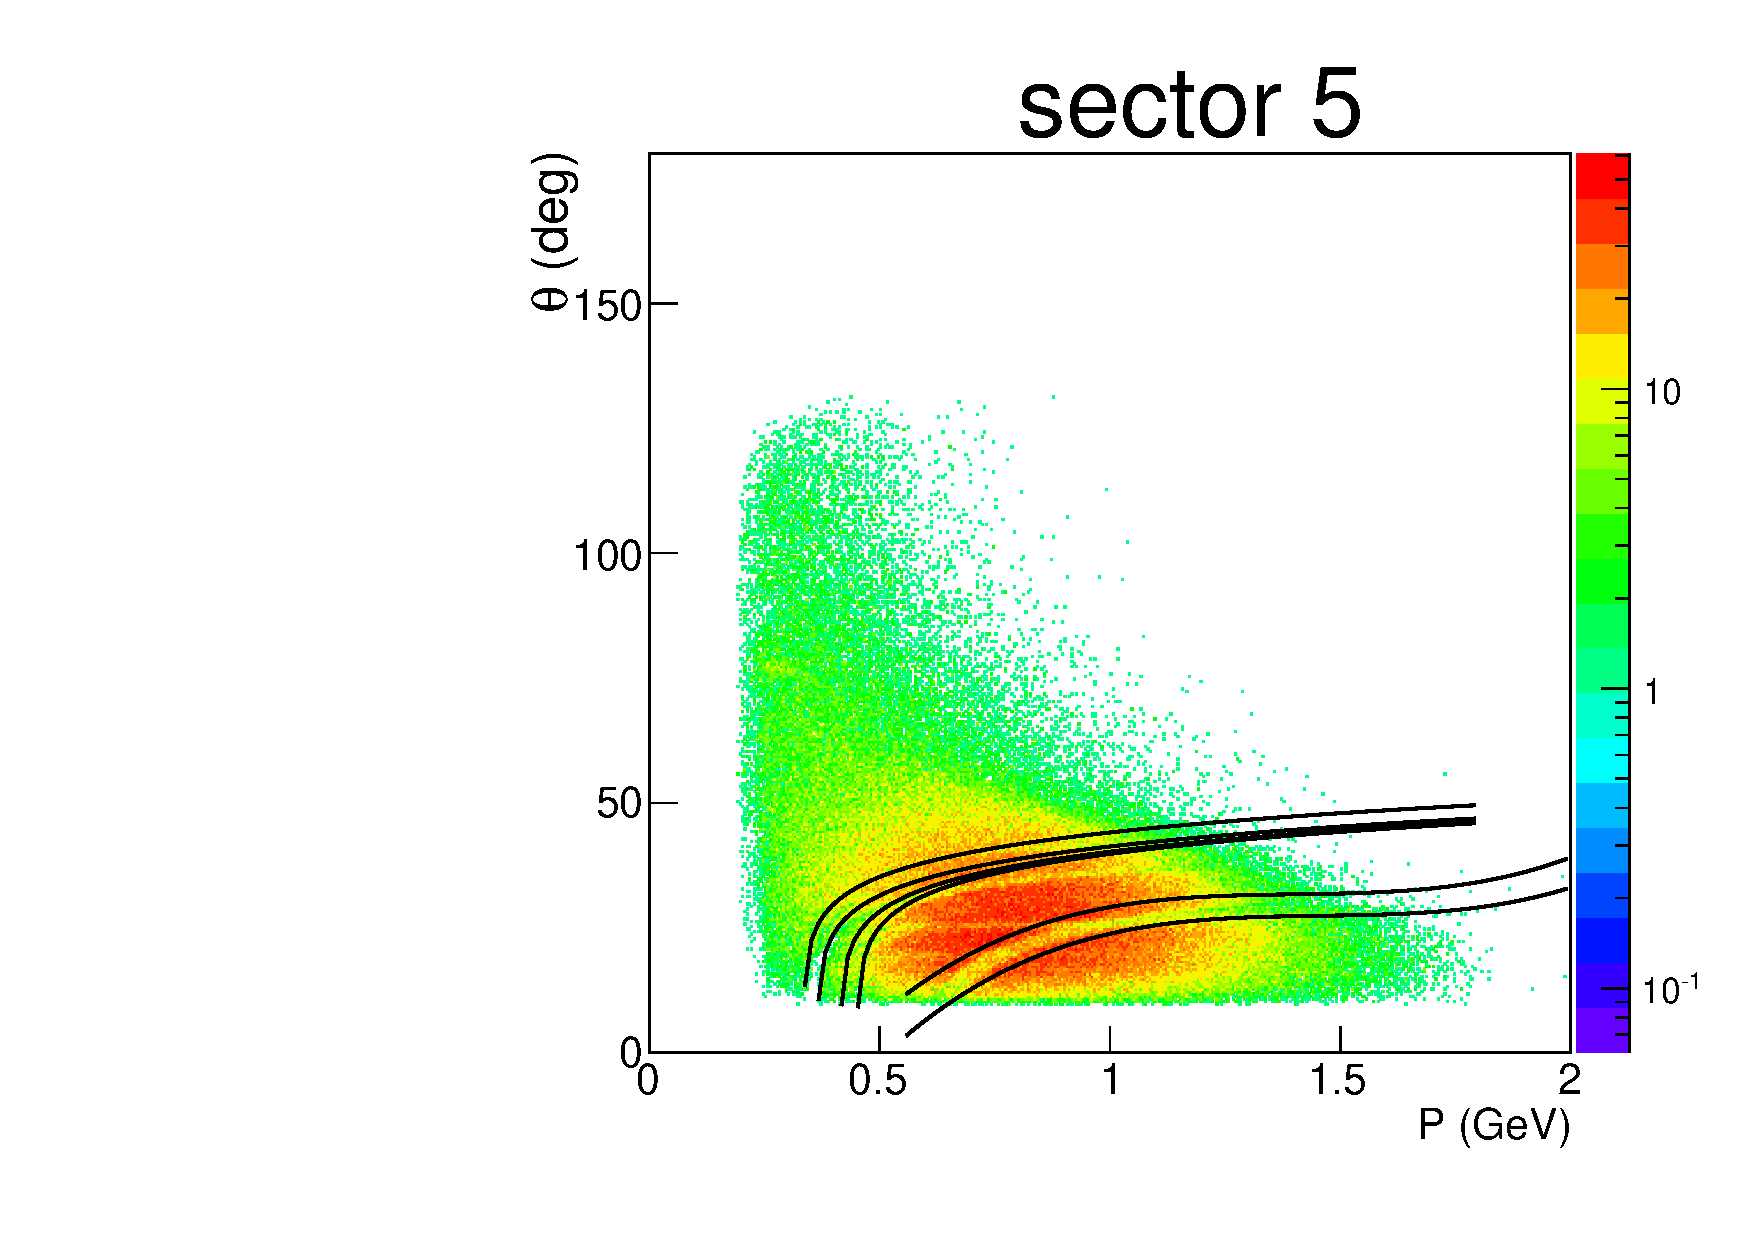
\includegraphics[width=5cm]{pictures/other_cuts/fiduch/th_vs_p_p/p_th_vs_p_sector5.pdf}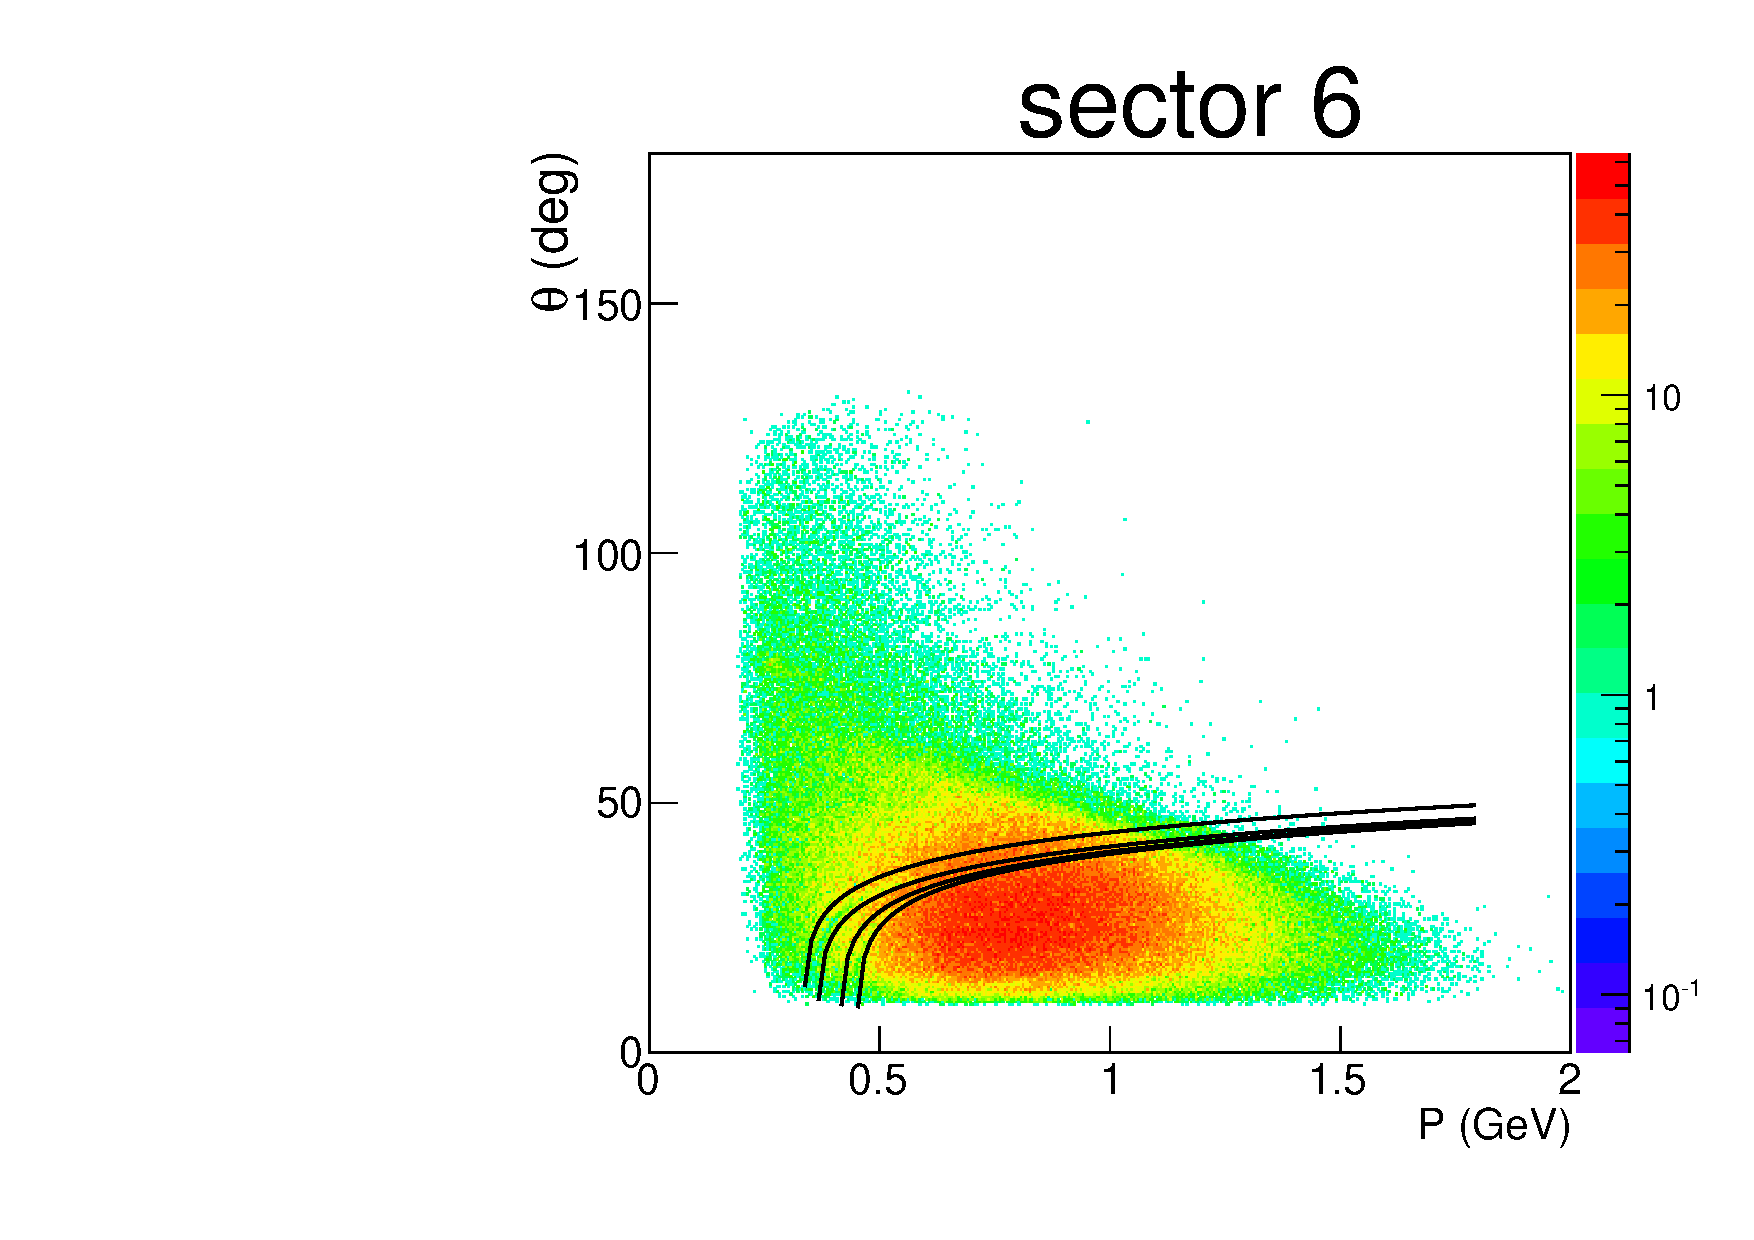
\includegraphics[width=5cm]{pictures/other_cuts/fiduch/th_vs_p_p/p_th_vs_p_sector6.pdf}
\end{framed}
\end{minipage}
\begin{minipage}{.99\textwidth}
\begin{framed}
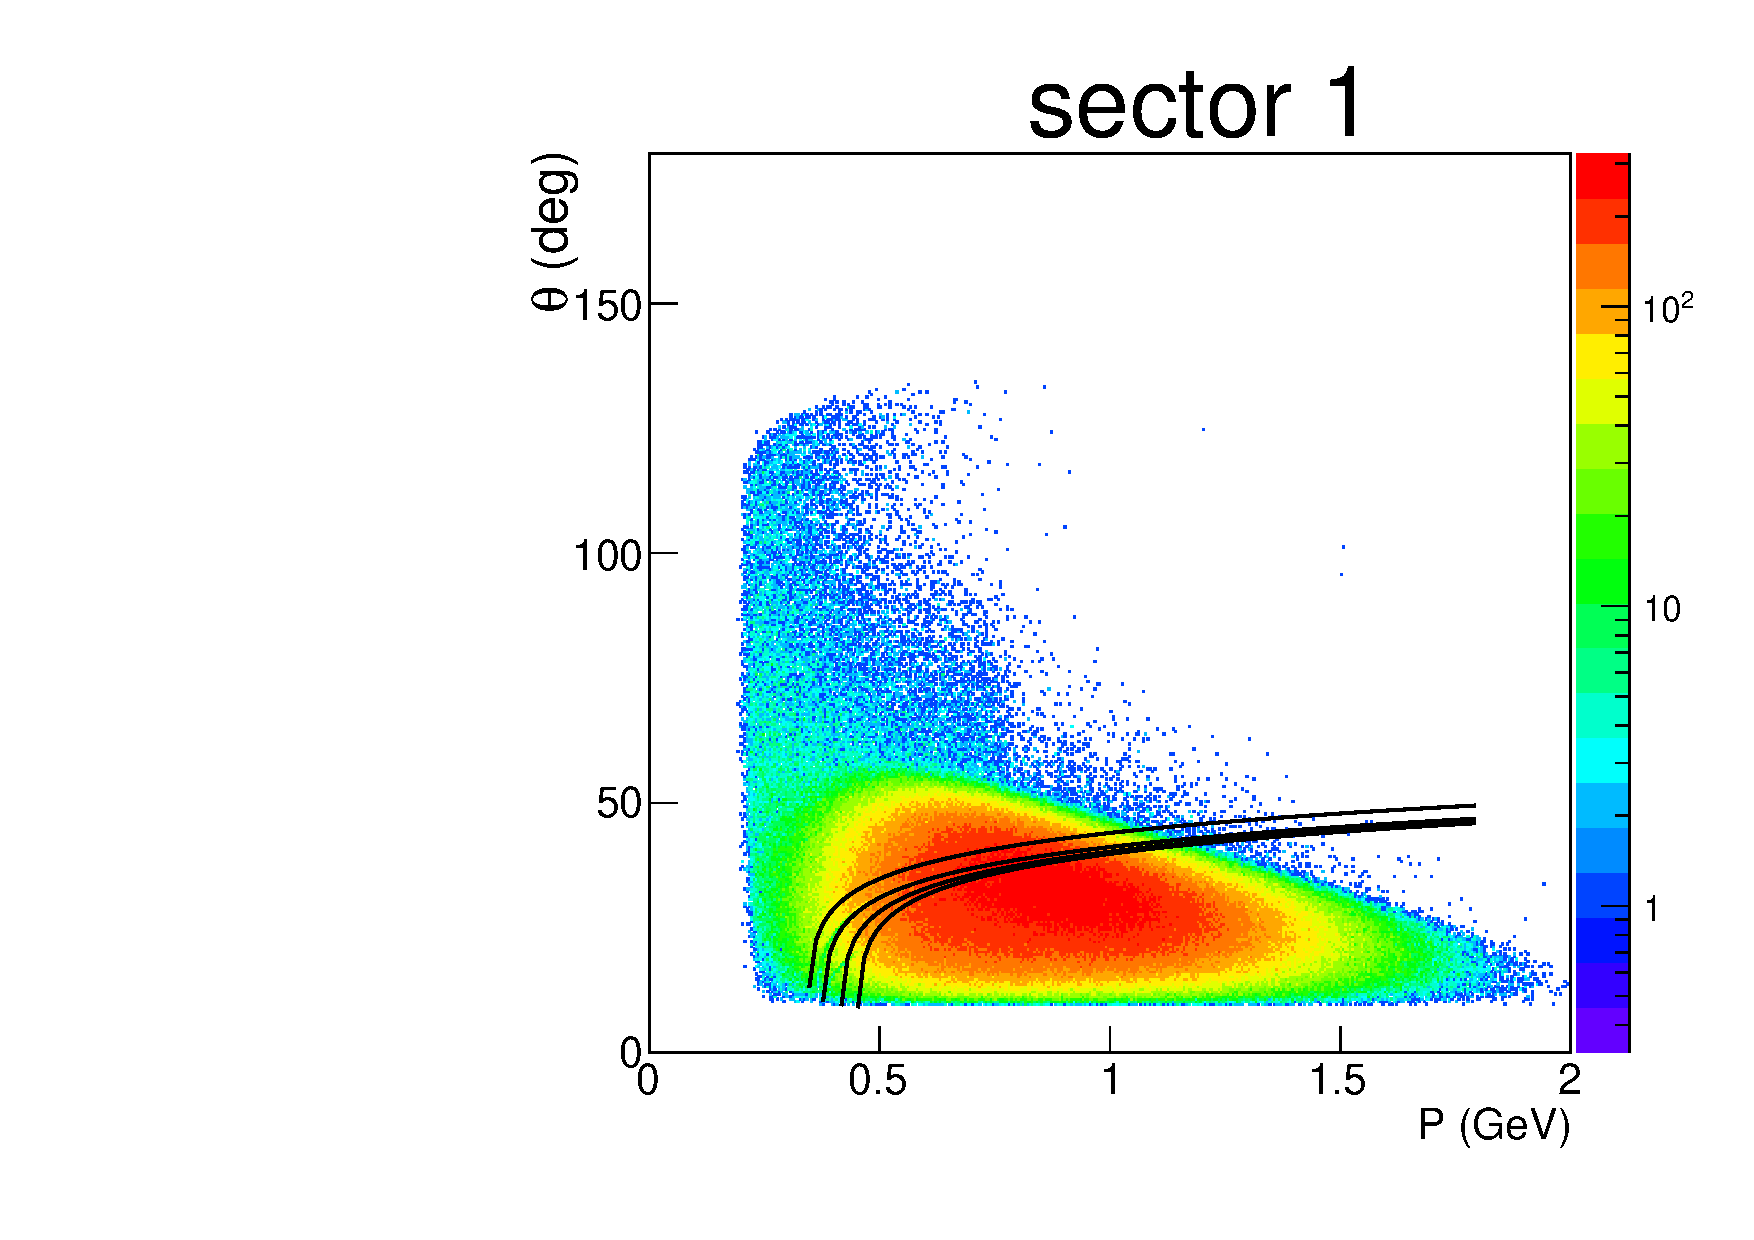
\includegraphics[width=5cm]{pictures/other_cuts/fiduch/th_vs_p_p_sim/p_th_vs_p_sim_sector1.pdf}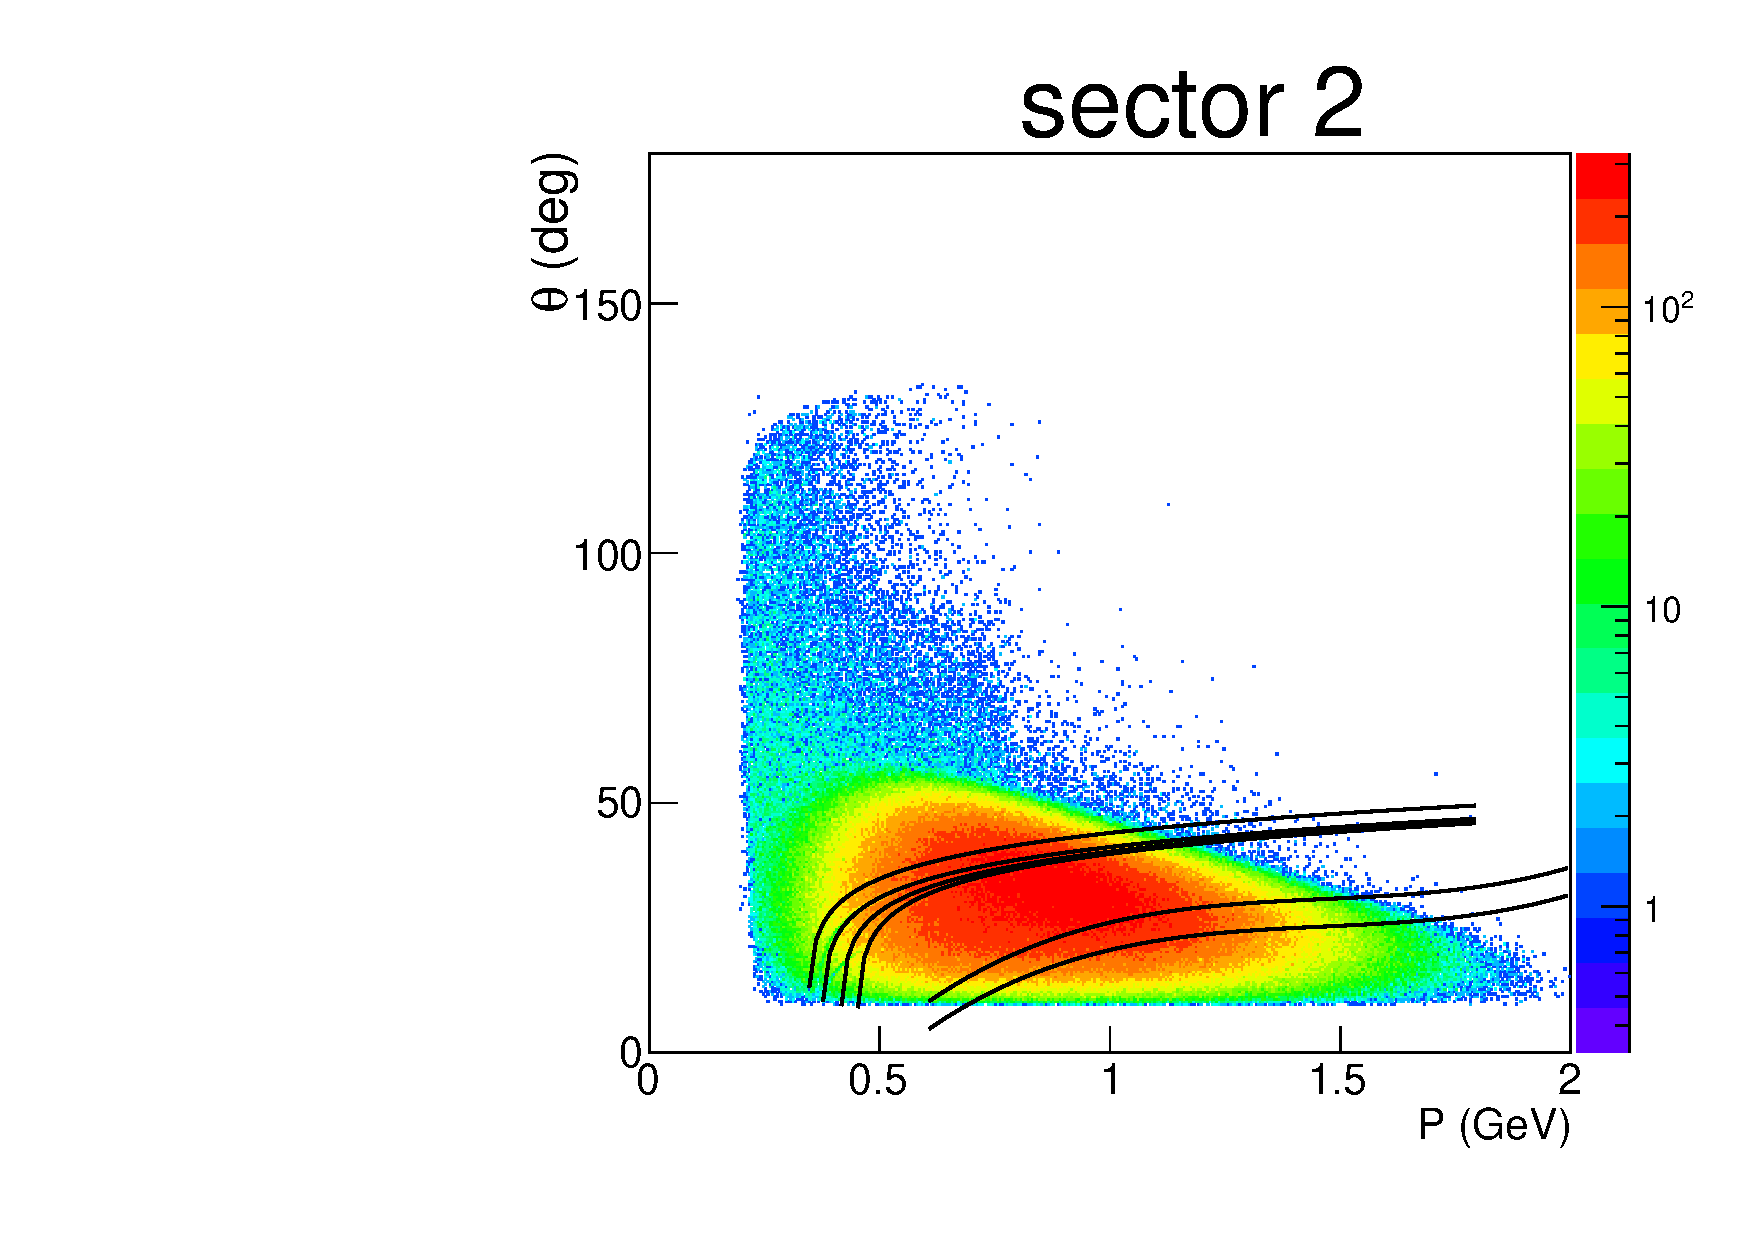
\includegraphics[width=5cm]{pictures/other_cuts/fiduch/th_vs_p_p_sim/p_th_vs_p_sim_sector2.pdf}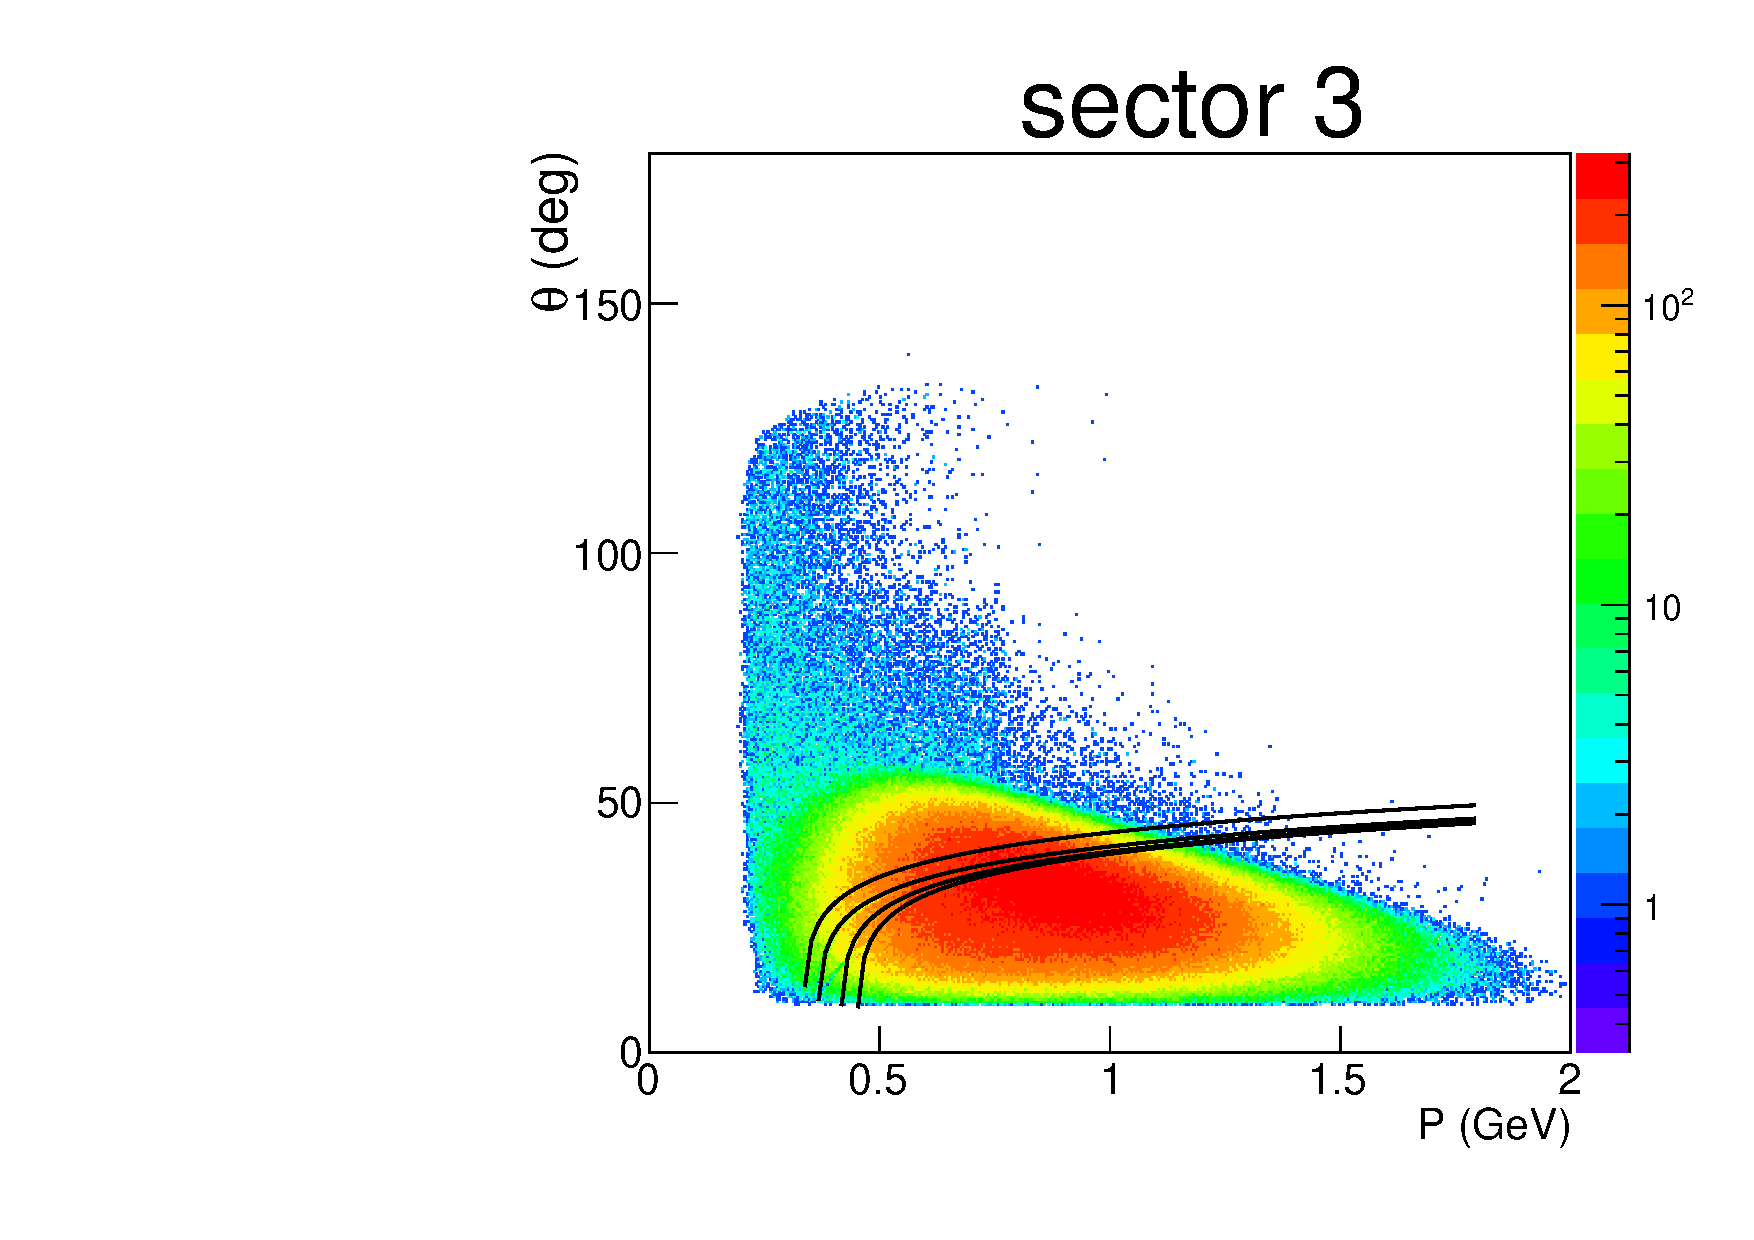
\includegraphics[width=5cm]{pictures/other_cuts/fiduch/th_vs_p_p_sim/p_th_vs_p_sim_sector3.pdf}
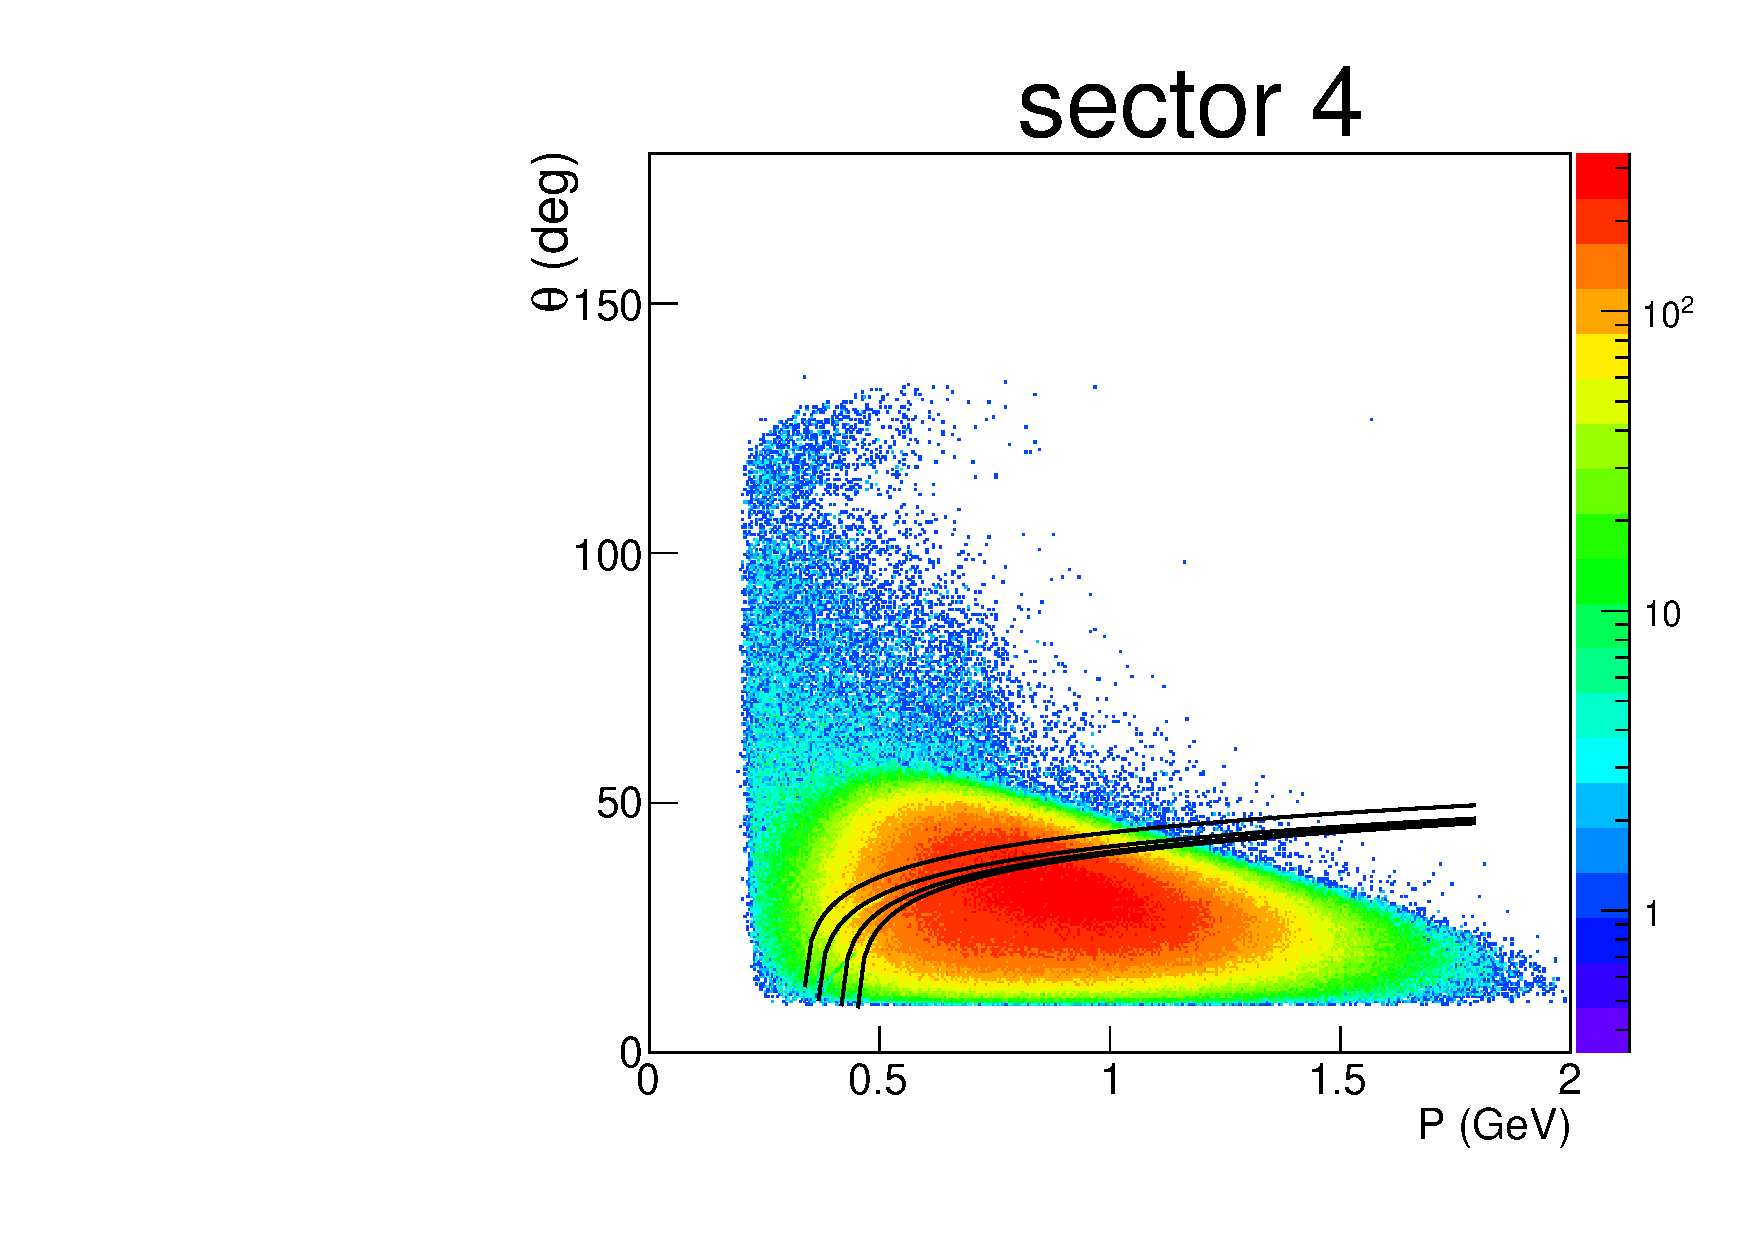
\includegraphics[width=5cm]{pictures/other_cuts/fiduch/th_vs_p_p_sim/p_th_vs_p_sim_sector4.pdf}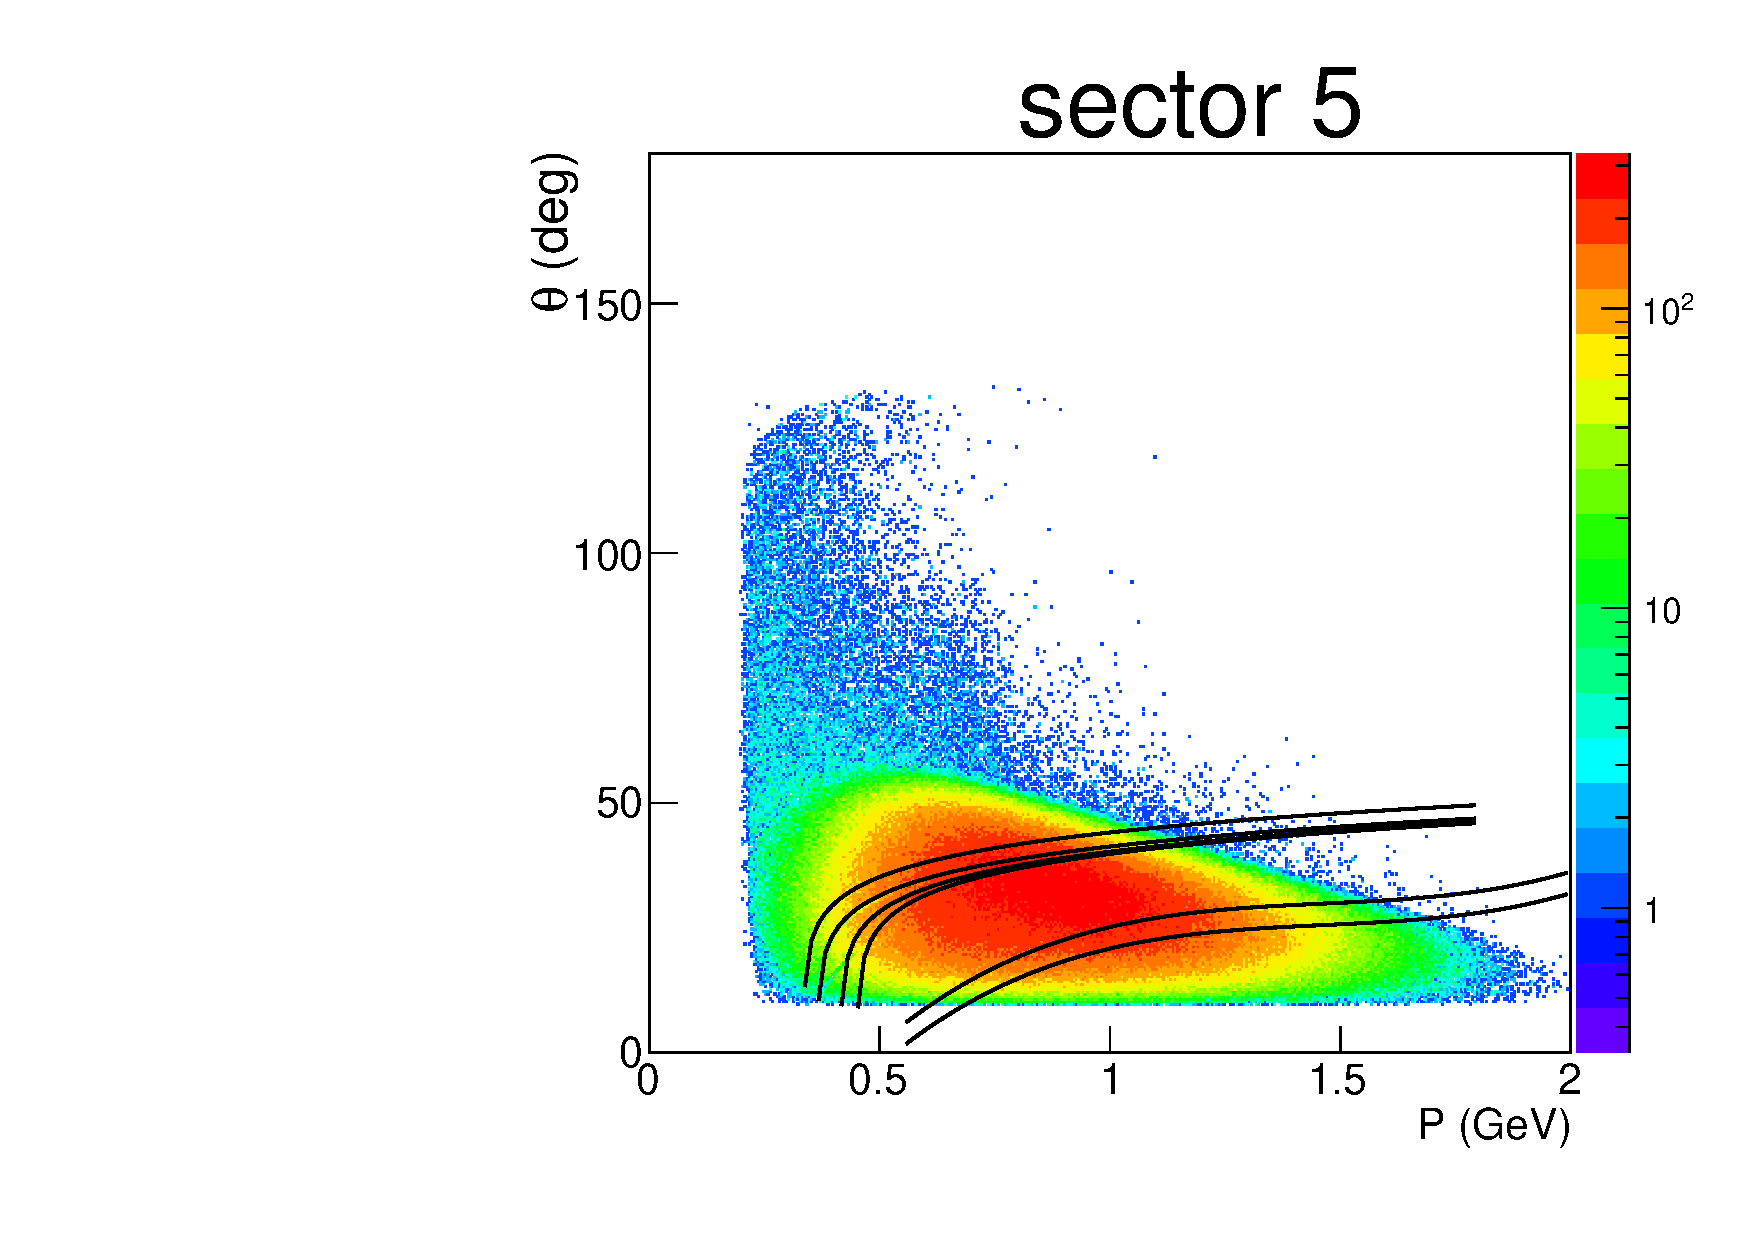
\includegraphics[width=5cm]{pictures/other_cuts/fiduch/th_vs_p_p_sim/p_th_vs_p_sim_sector5.pdf}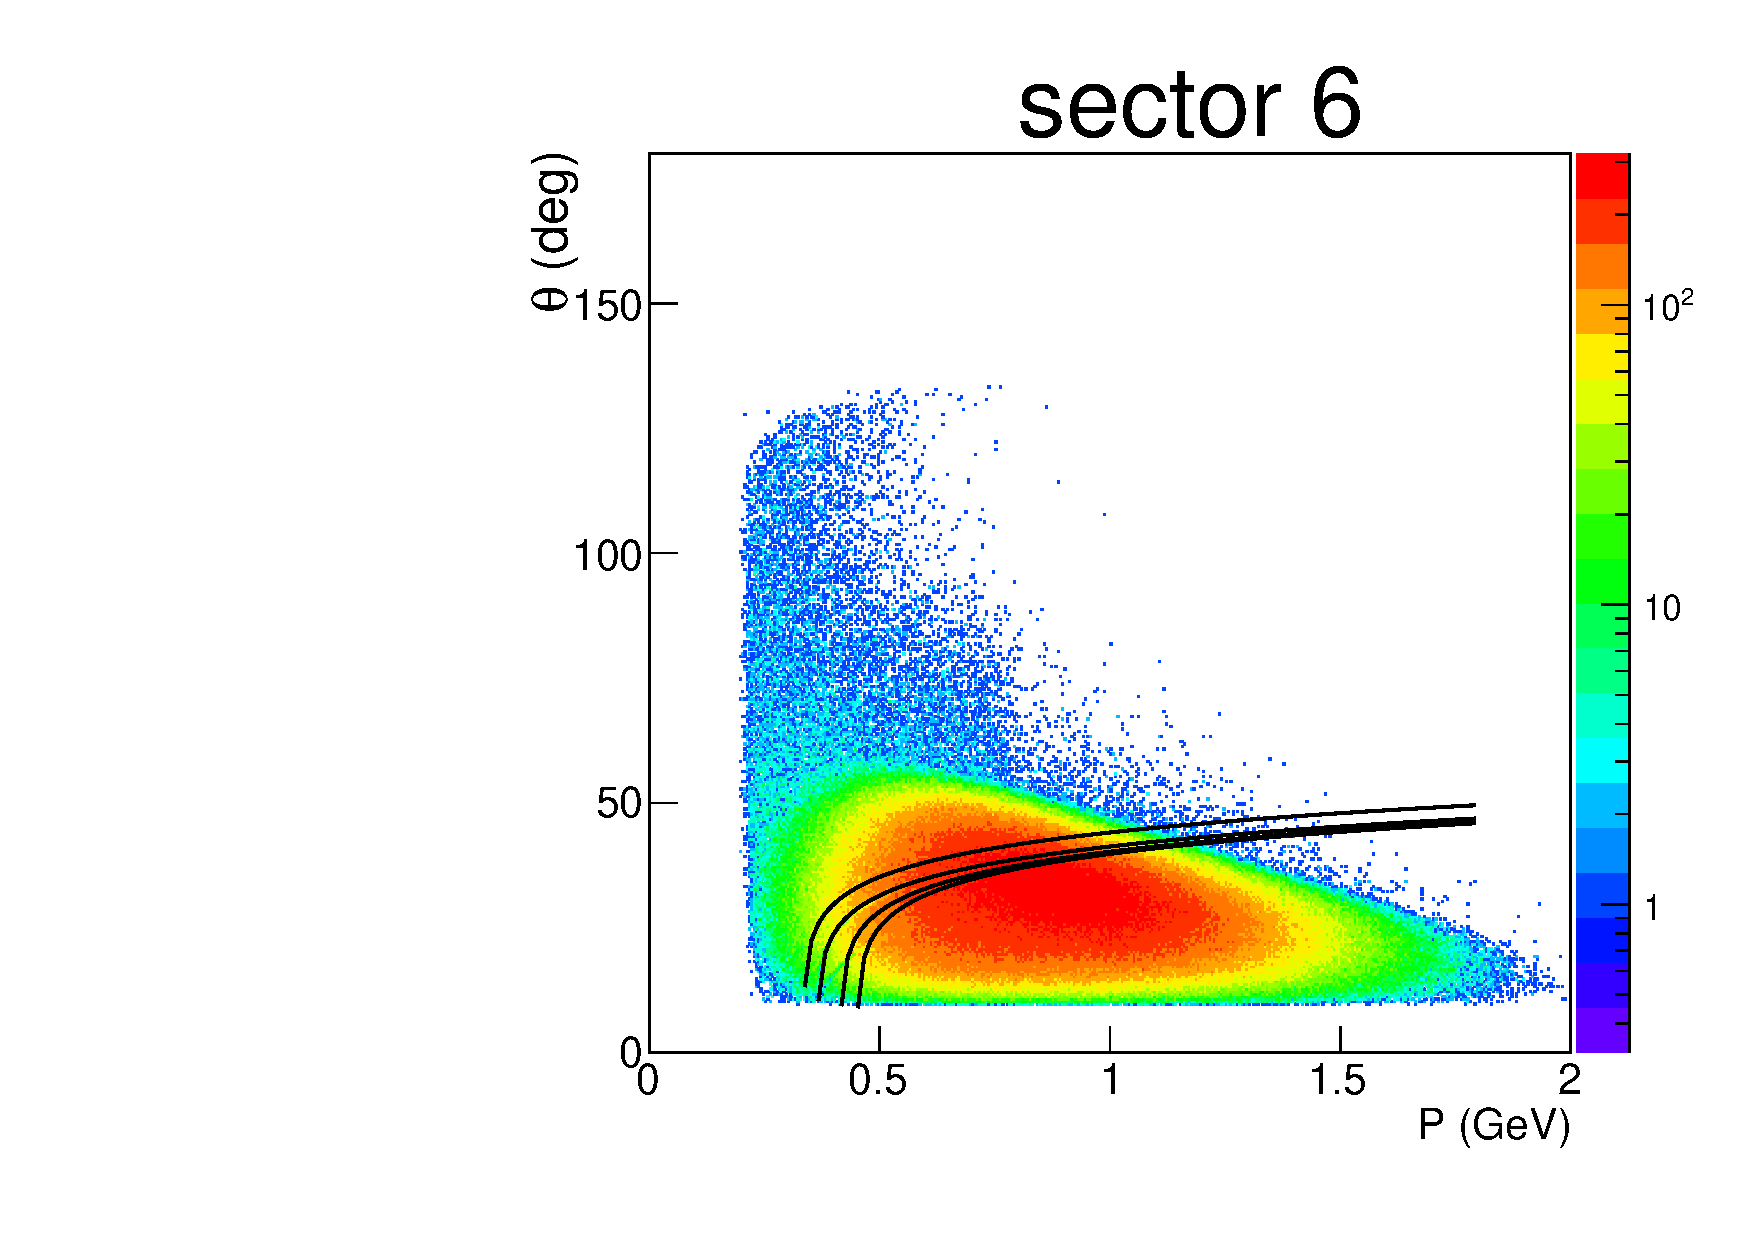
\includegraphics[width=5cm]{pictures/other_cuts/fiduch/th_vs_p_p_sim/p_th_vs_p_sim_sector6.pdf}
\end{framed}
\end{minipage}
%\end{framed}
\caption{\small $\theta$ versus momentum distributions for real proton events (upper frame)  and for Monte Carlo events (lower frame) for all six CLAS sectors. Black curves show cuts applied to remove inefficient areas. \label{fig:other_cuts_positive_th_vs_p_protons}}
\end{center}
\end{figure}


\begin{figure}[htp]
\begin{center}
%\begin{framed}
\begin{minipage}{.99\textwidth}
\begin{framed}
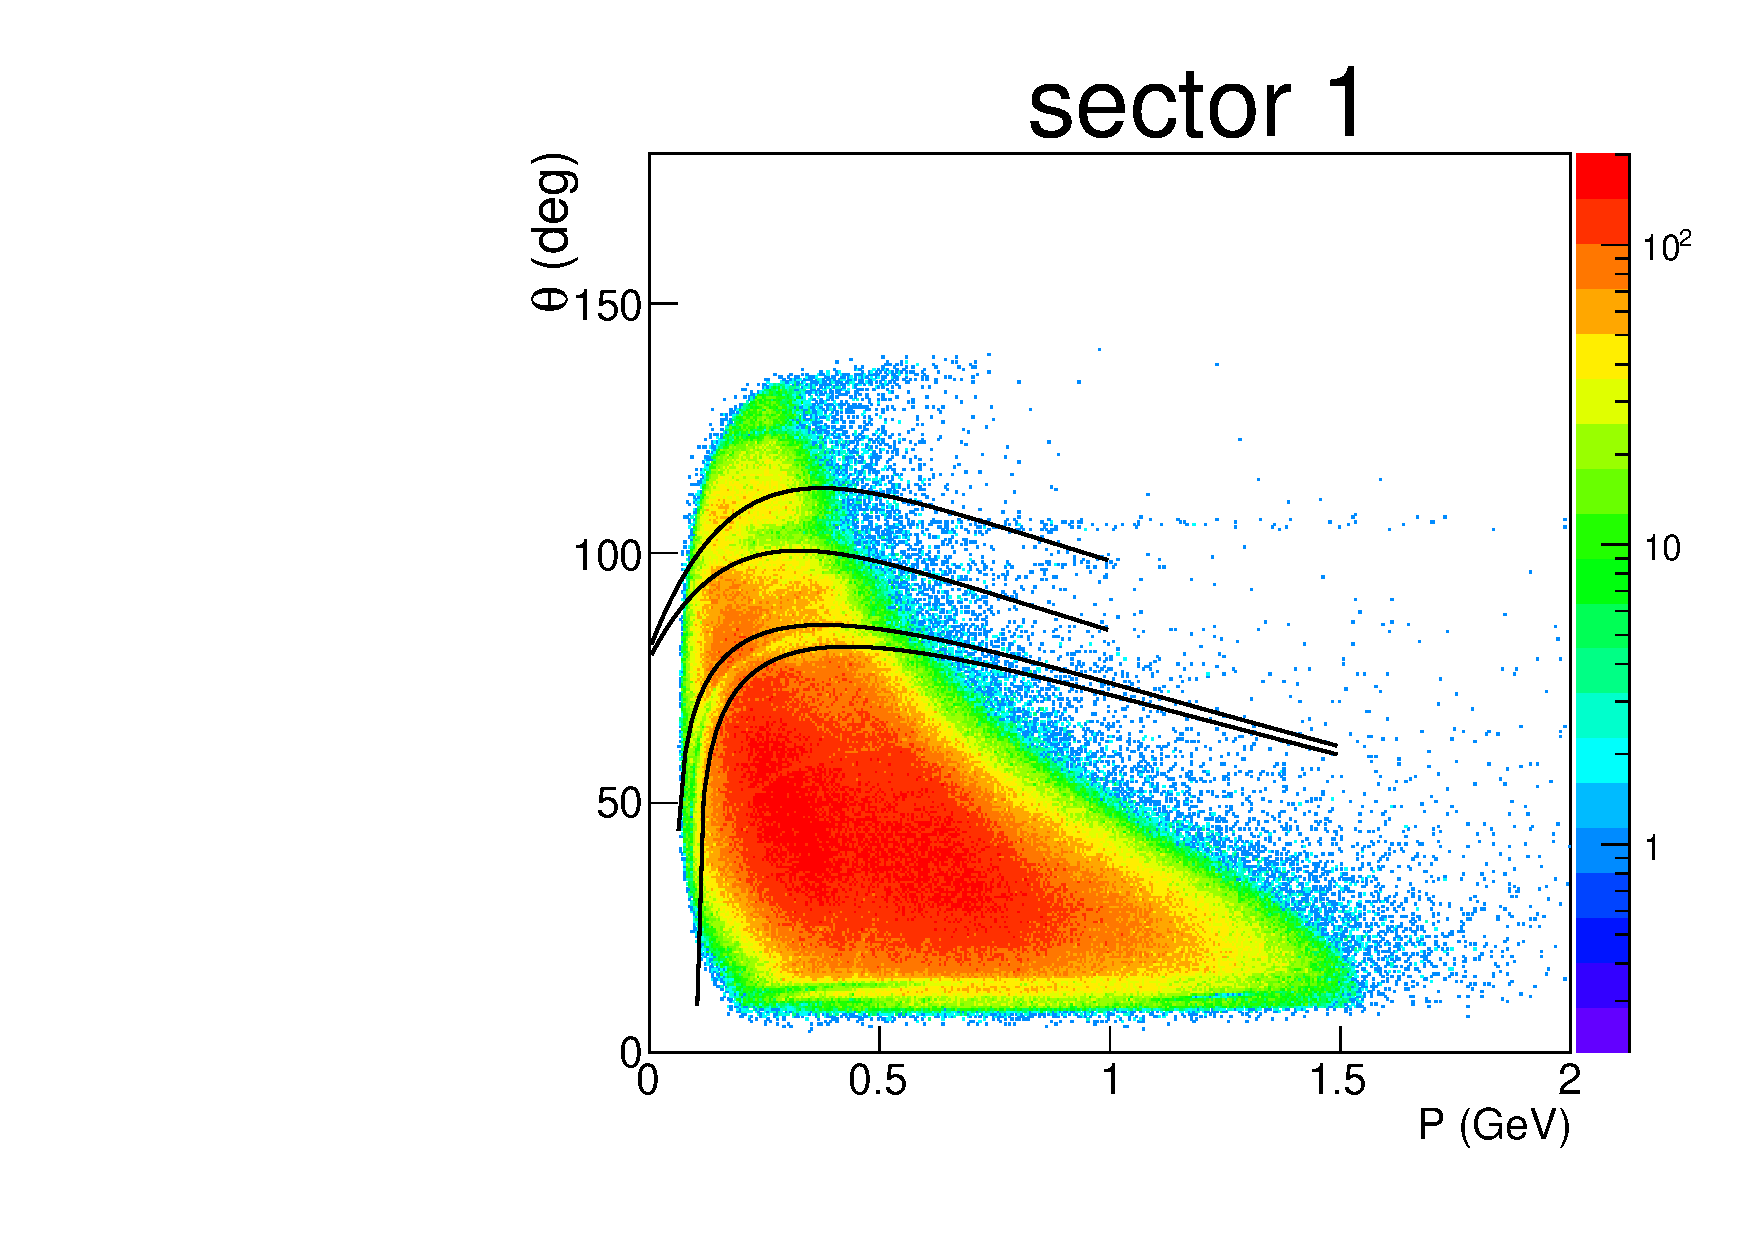
\includegraphics[width=5cm]{pictures/other_cuts/fiduch/th_vs_p_pip/pip_th_vs_p_sector1.pdf}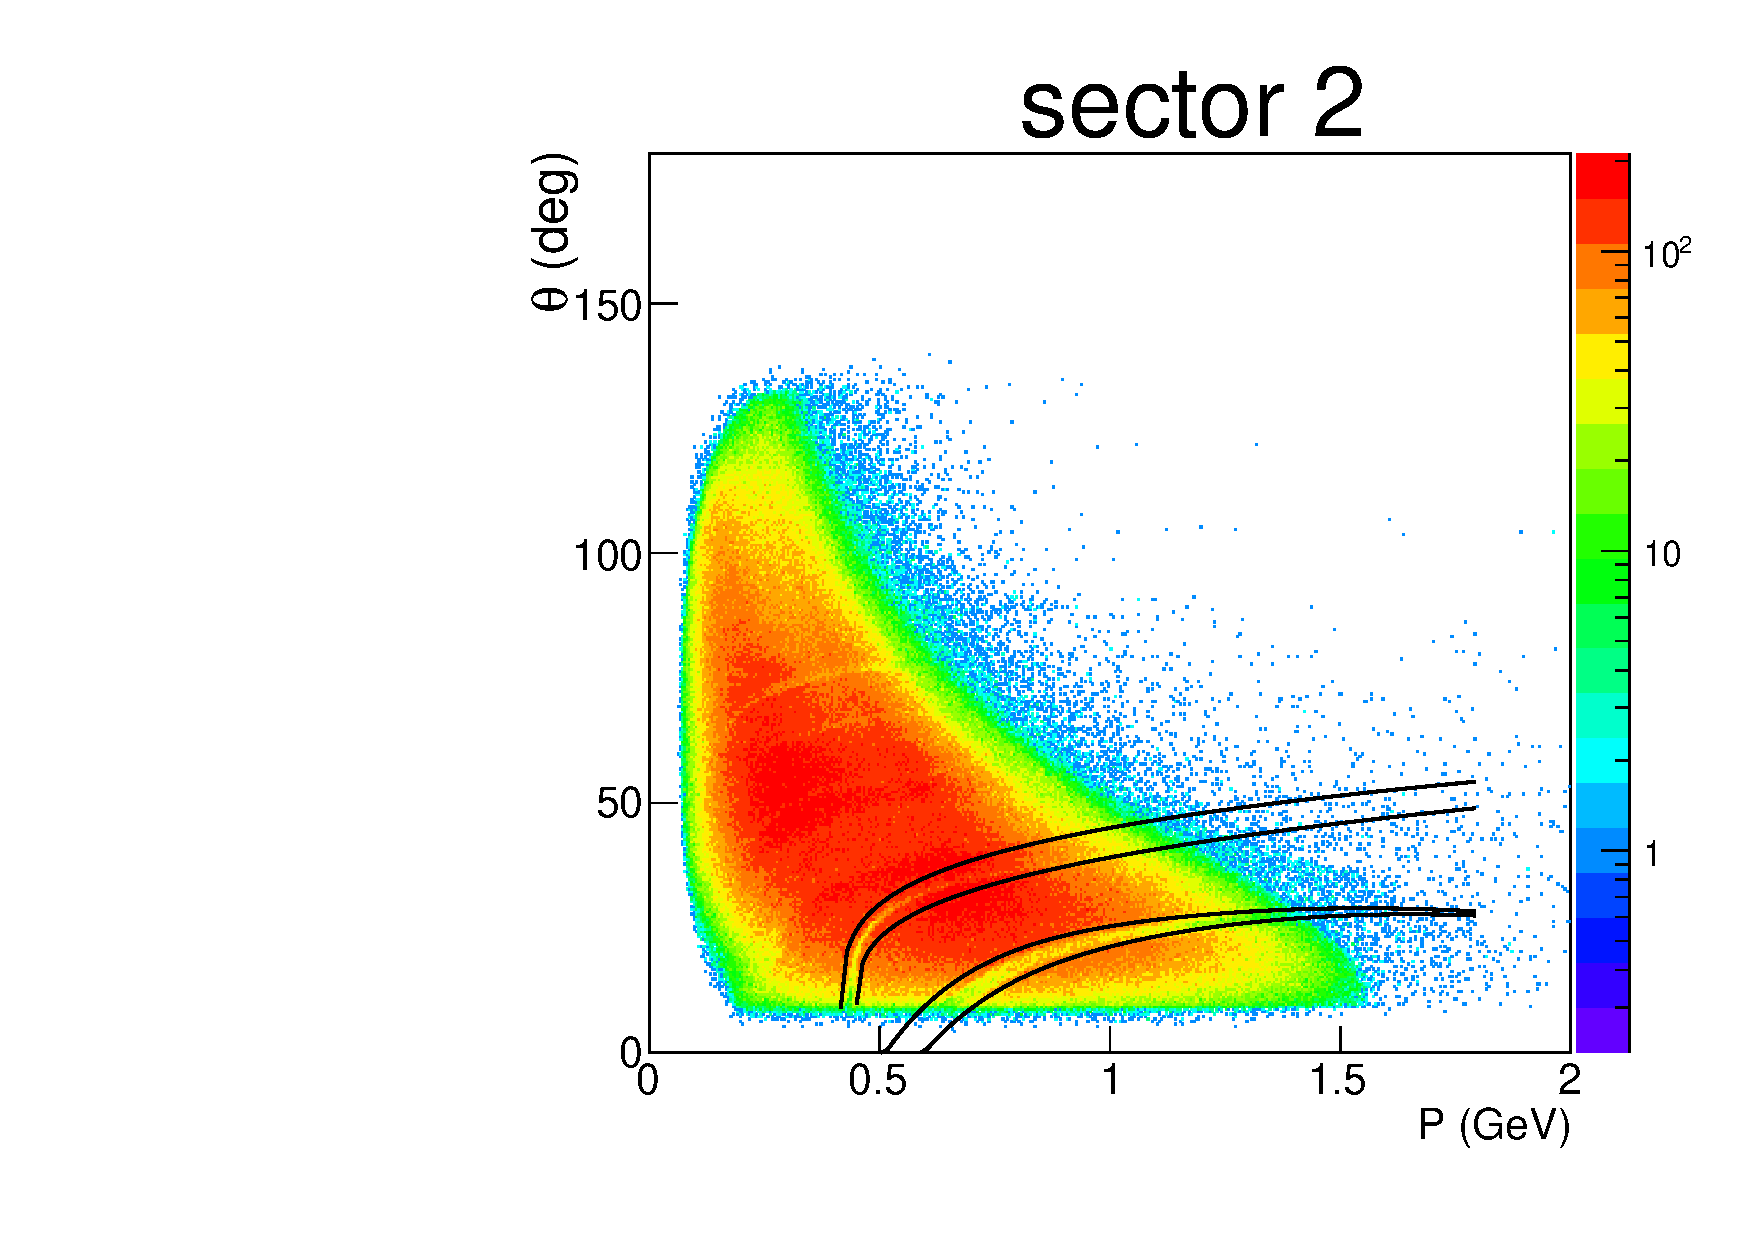
\includegraphics[width=5cm]{pictures/other_cuts/fiduch/th_vs_p_pip/pip_th_vs_p_sector2.pdf}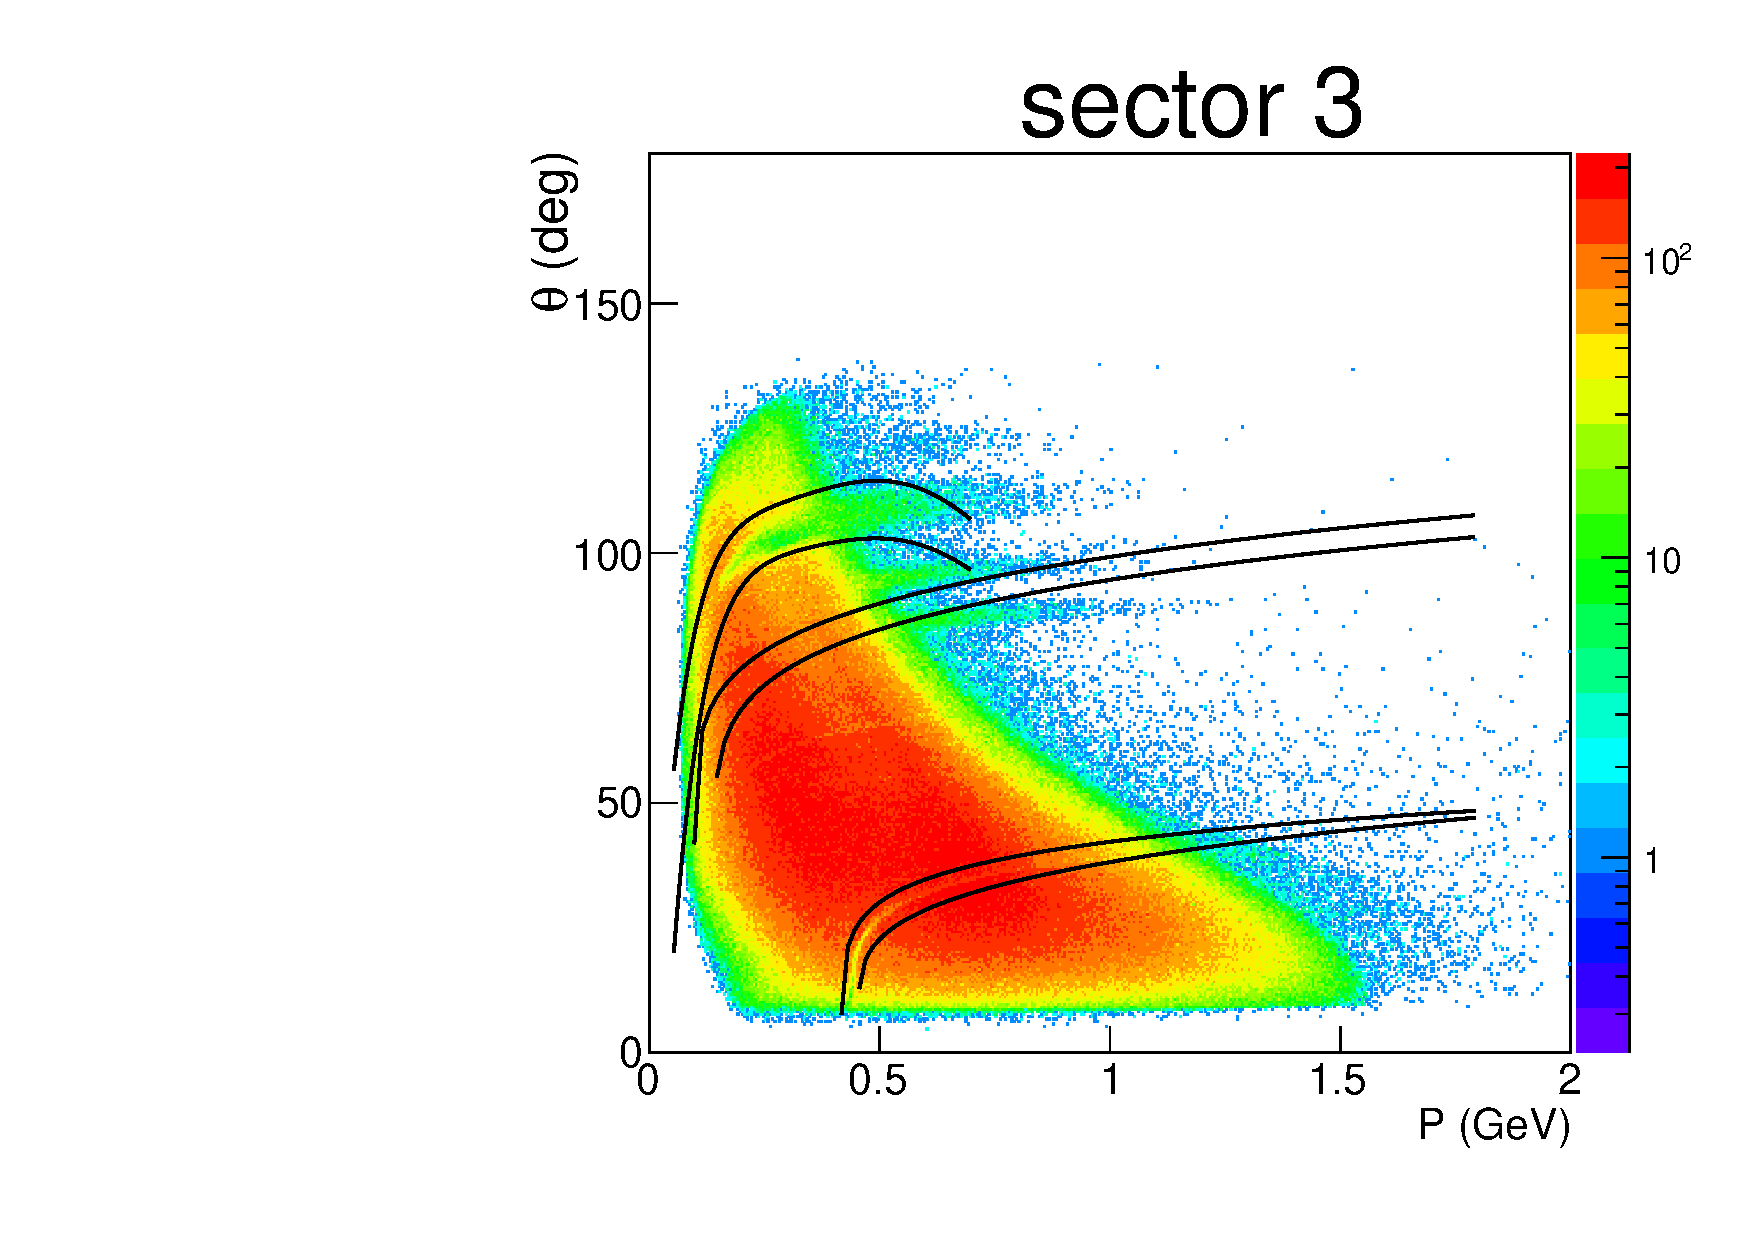
\includegraphics[width=5cm]{pictures/other_cuts/fiduch/th_vs_p_pip/pip_th_vs_p_sector3.pdf}
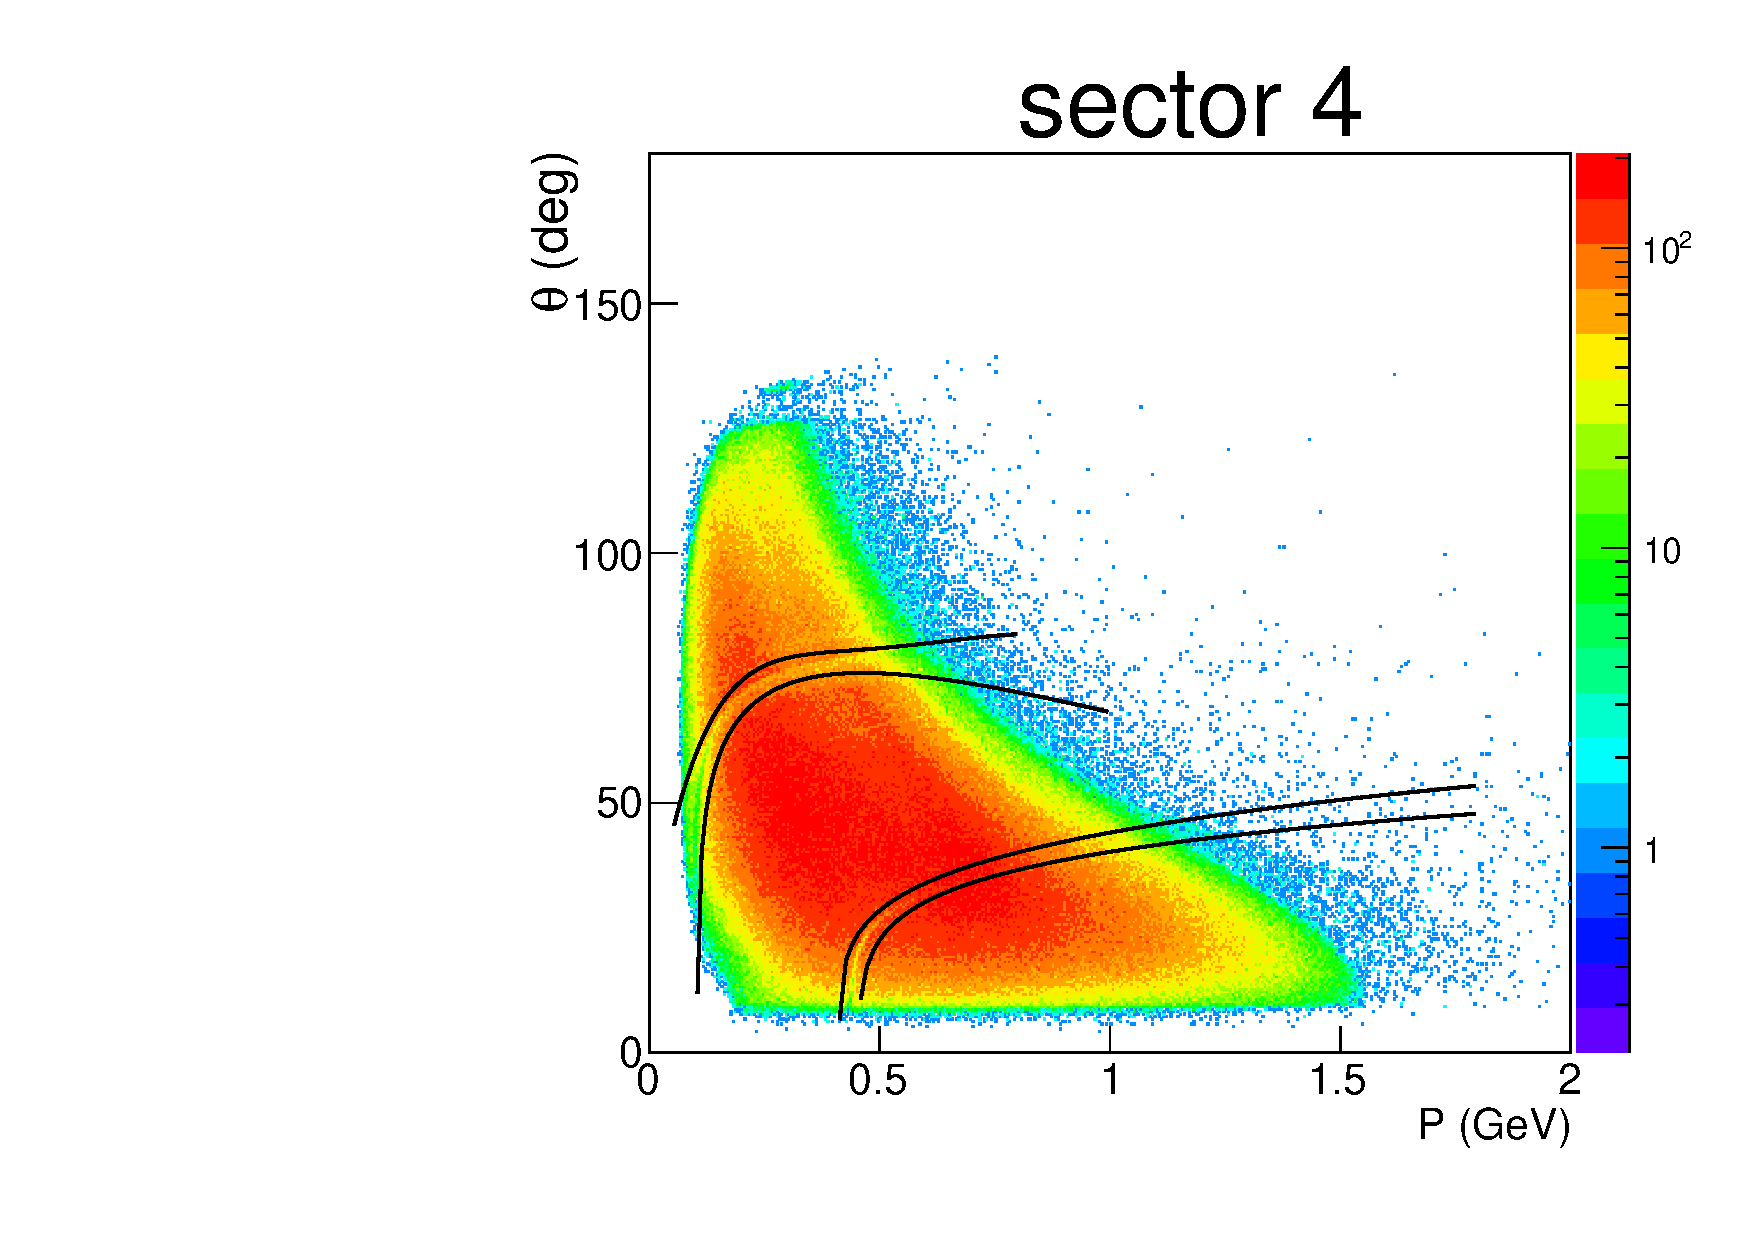
\includegraphics[width=5cm]{pictures/other_cuts/fiduch/th_vs_p_pip/pip_th_vs_p_sector4.pdf}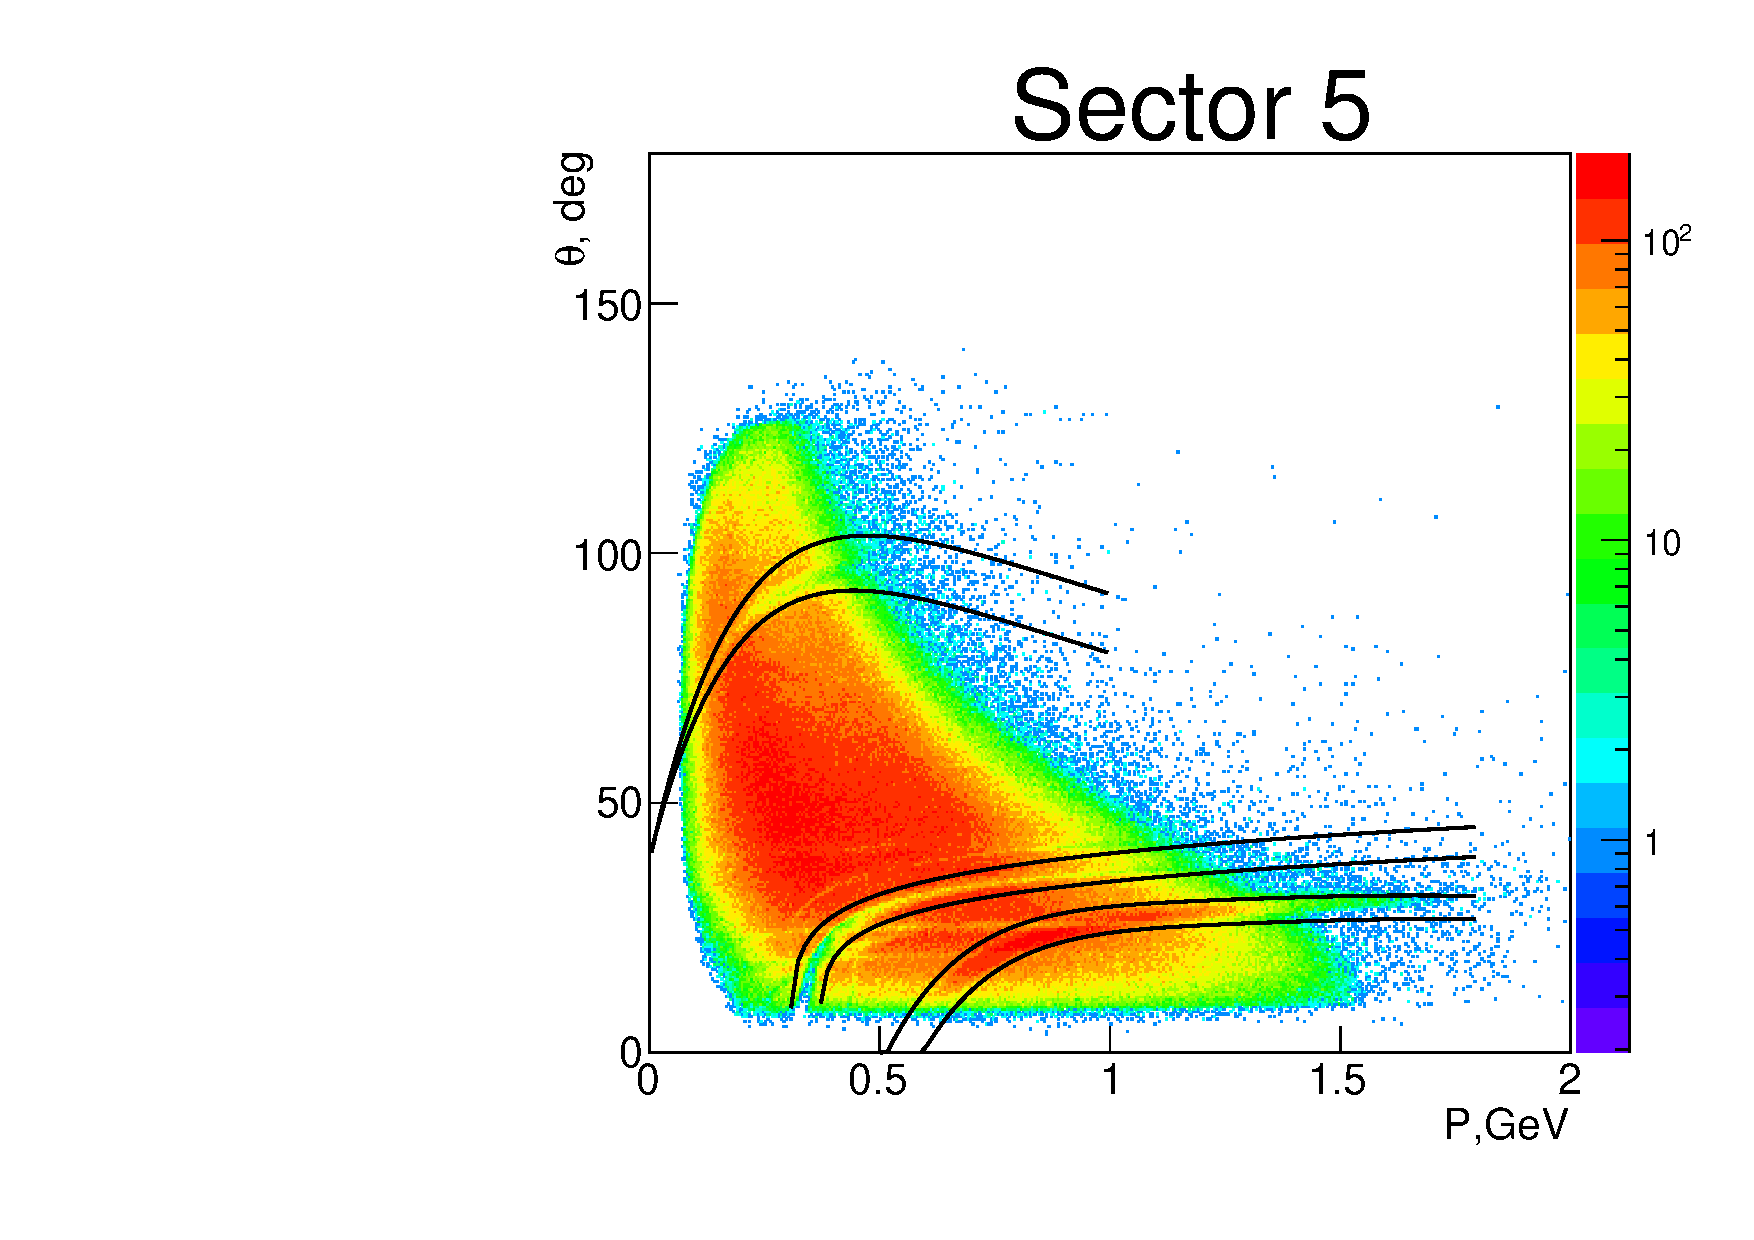
\includegraphics[width=5cm]{pictures/other_cuts/fiduch/th_vs_p_pip/pip_th_vs_p_sector5.pdf}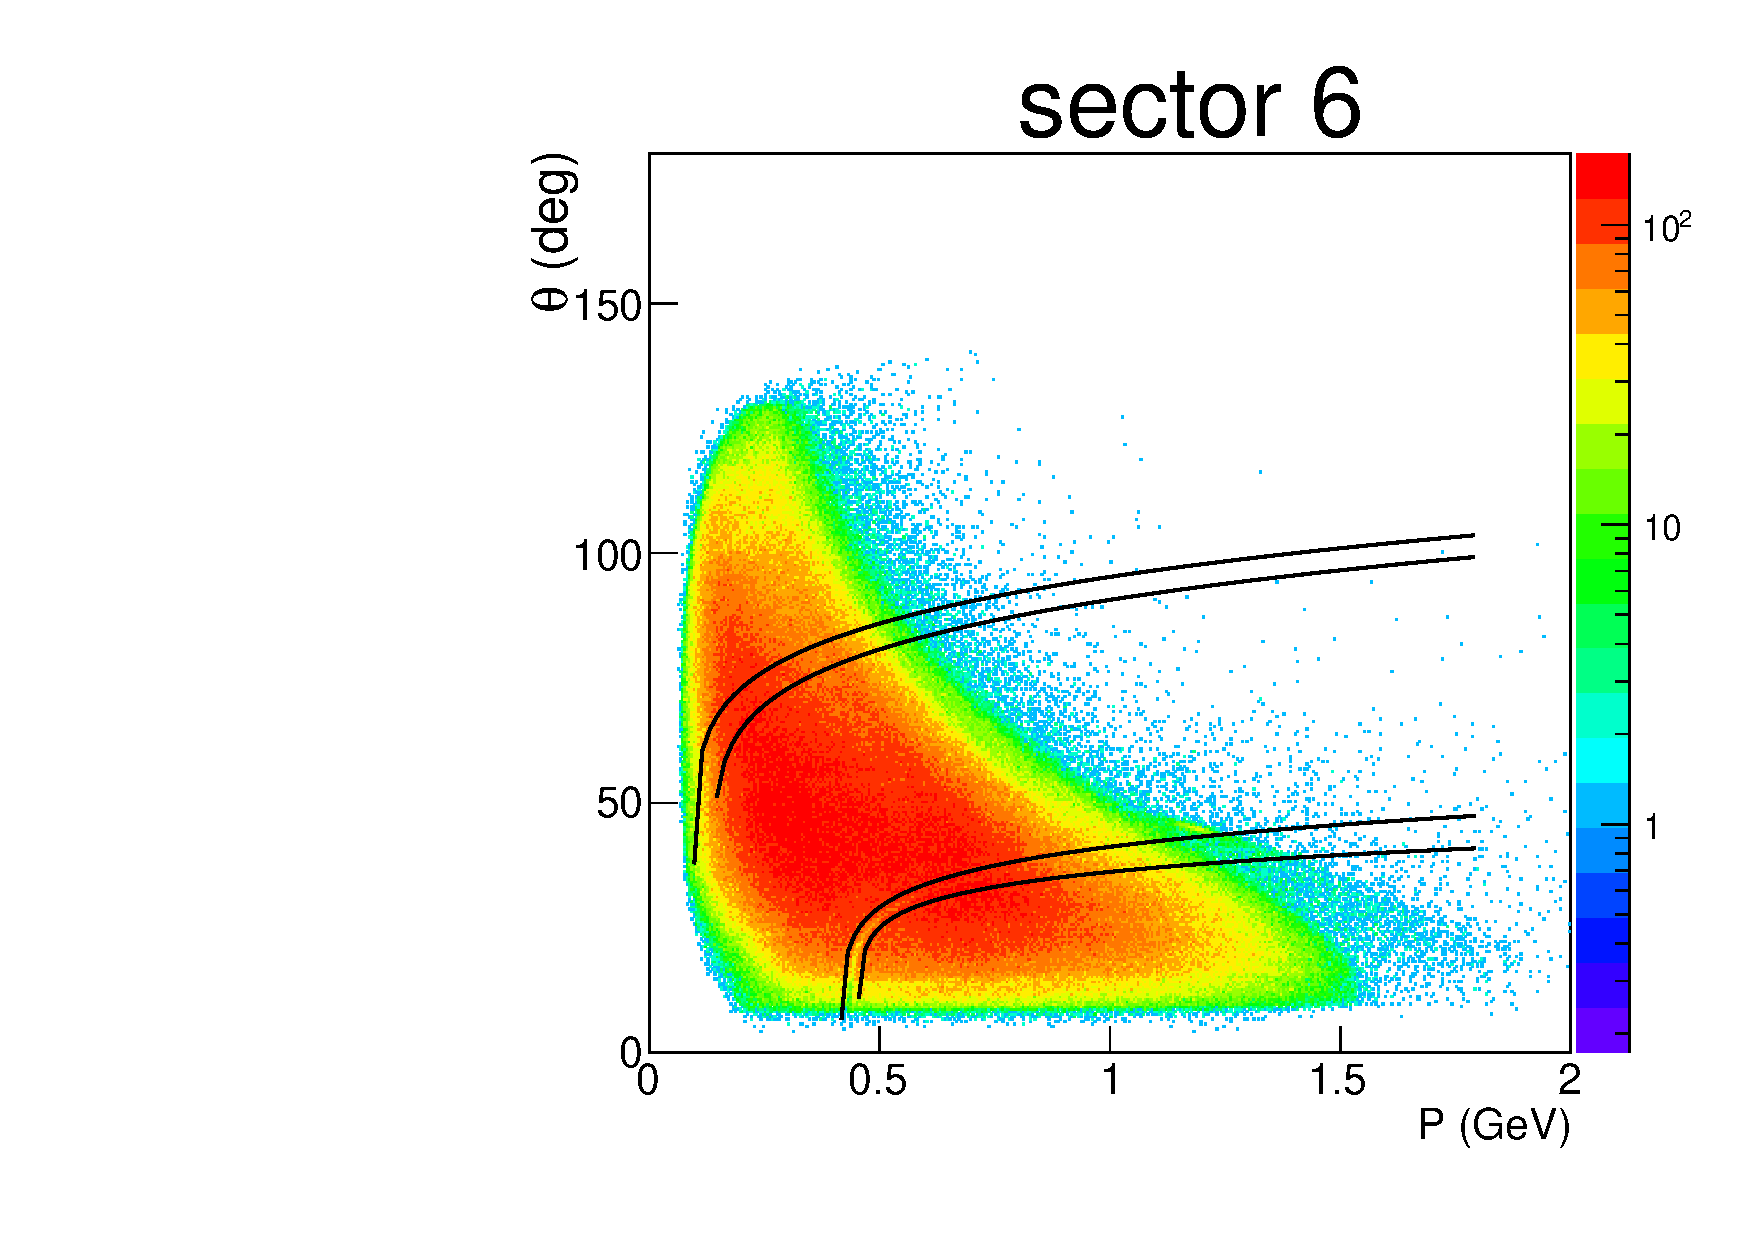
\includegraphics[width=5cm]{pictures/other_cuts/fiduch/th_vs_p_pip/pip_th_vs_p_sector6.pdf}
\end{framed}
\end{minipage}
\begin{minipage}{.99\textwidth}
\begin{framed}
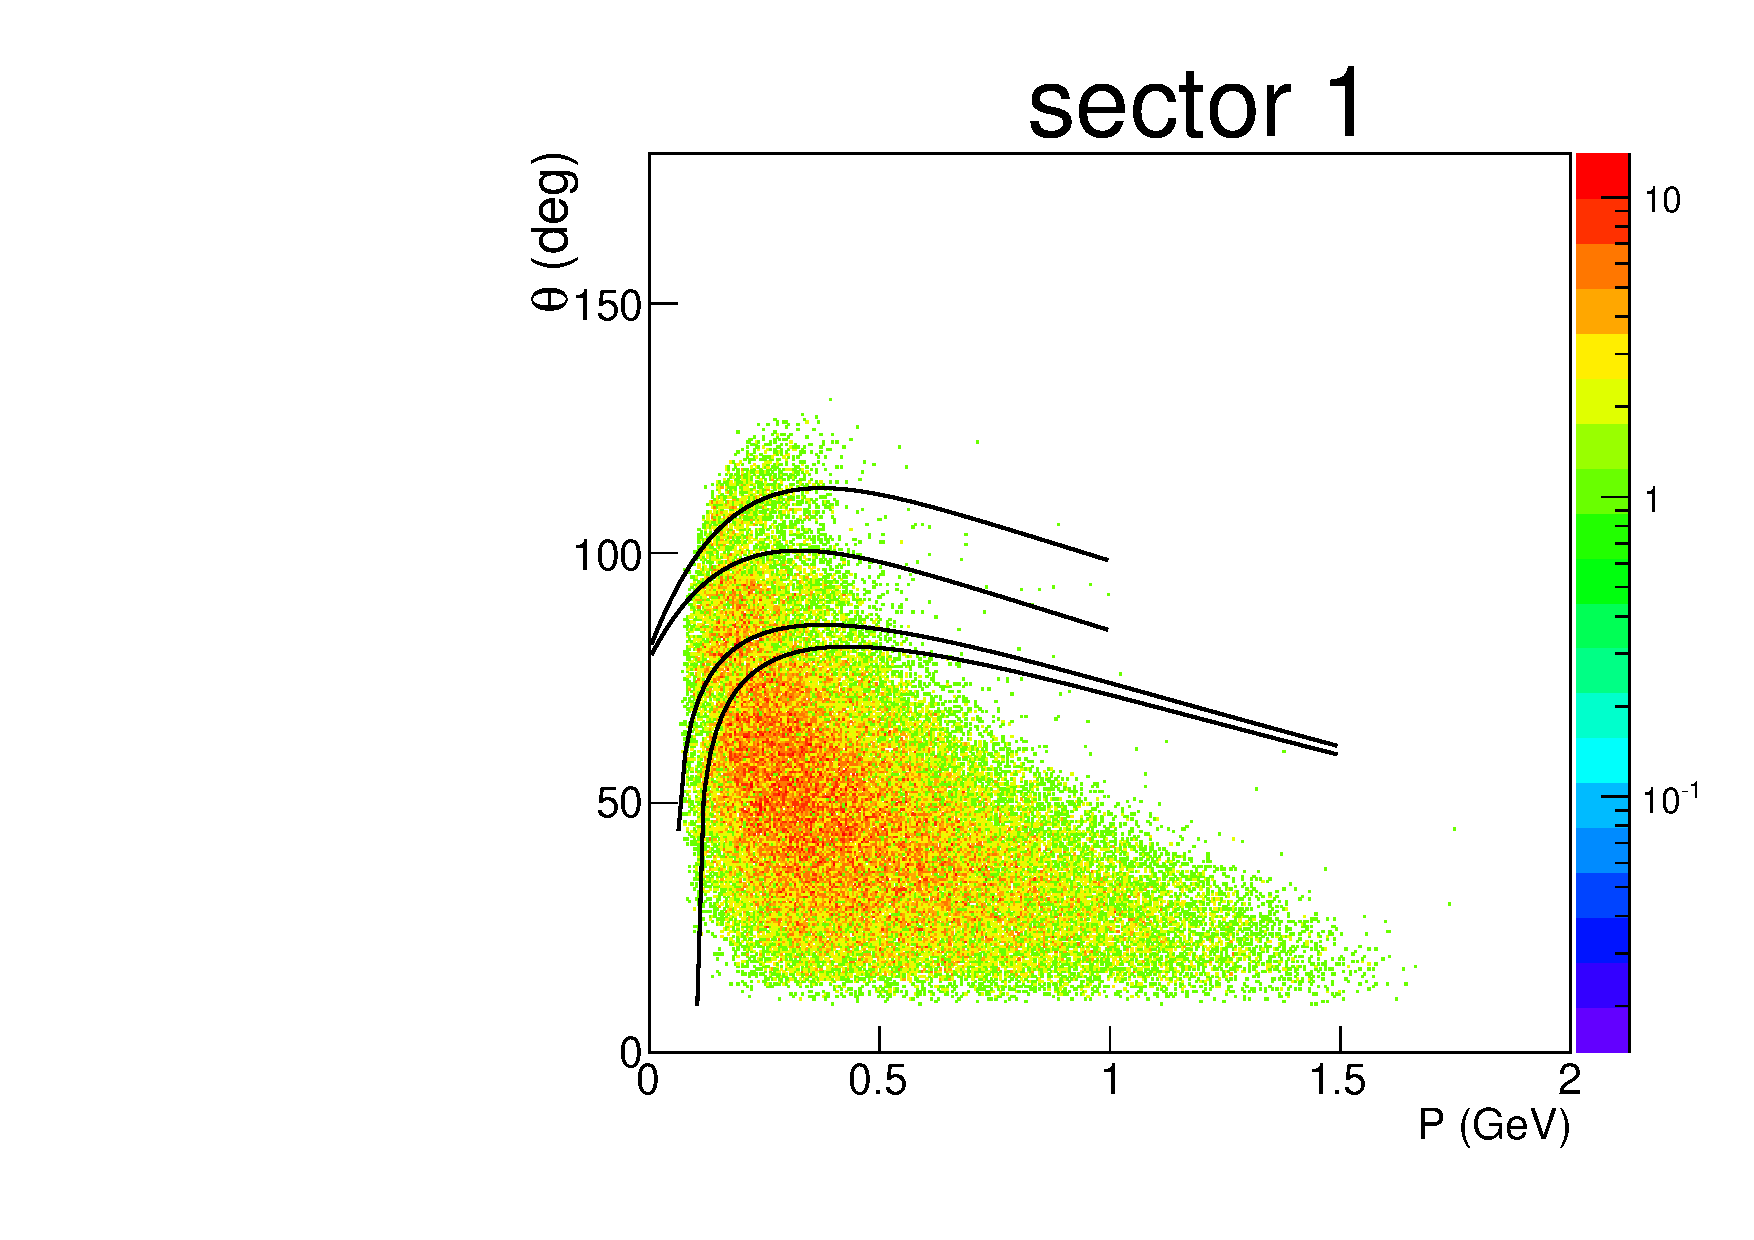
\includegraphics[width=5cm]{pictures/other_cuts/fiduch/th_vs_p_pip_sim/pip_th_vs_p_sim_sector1.pdf}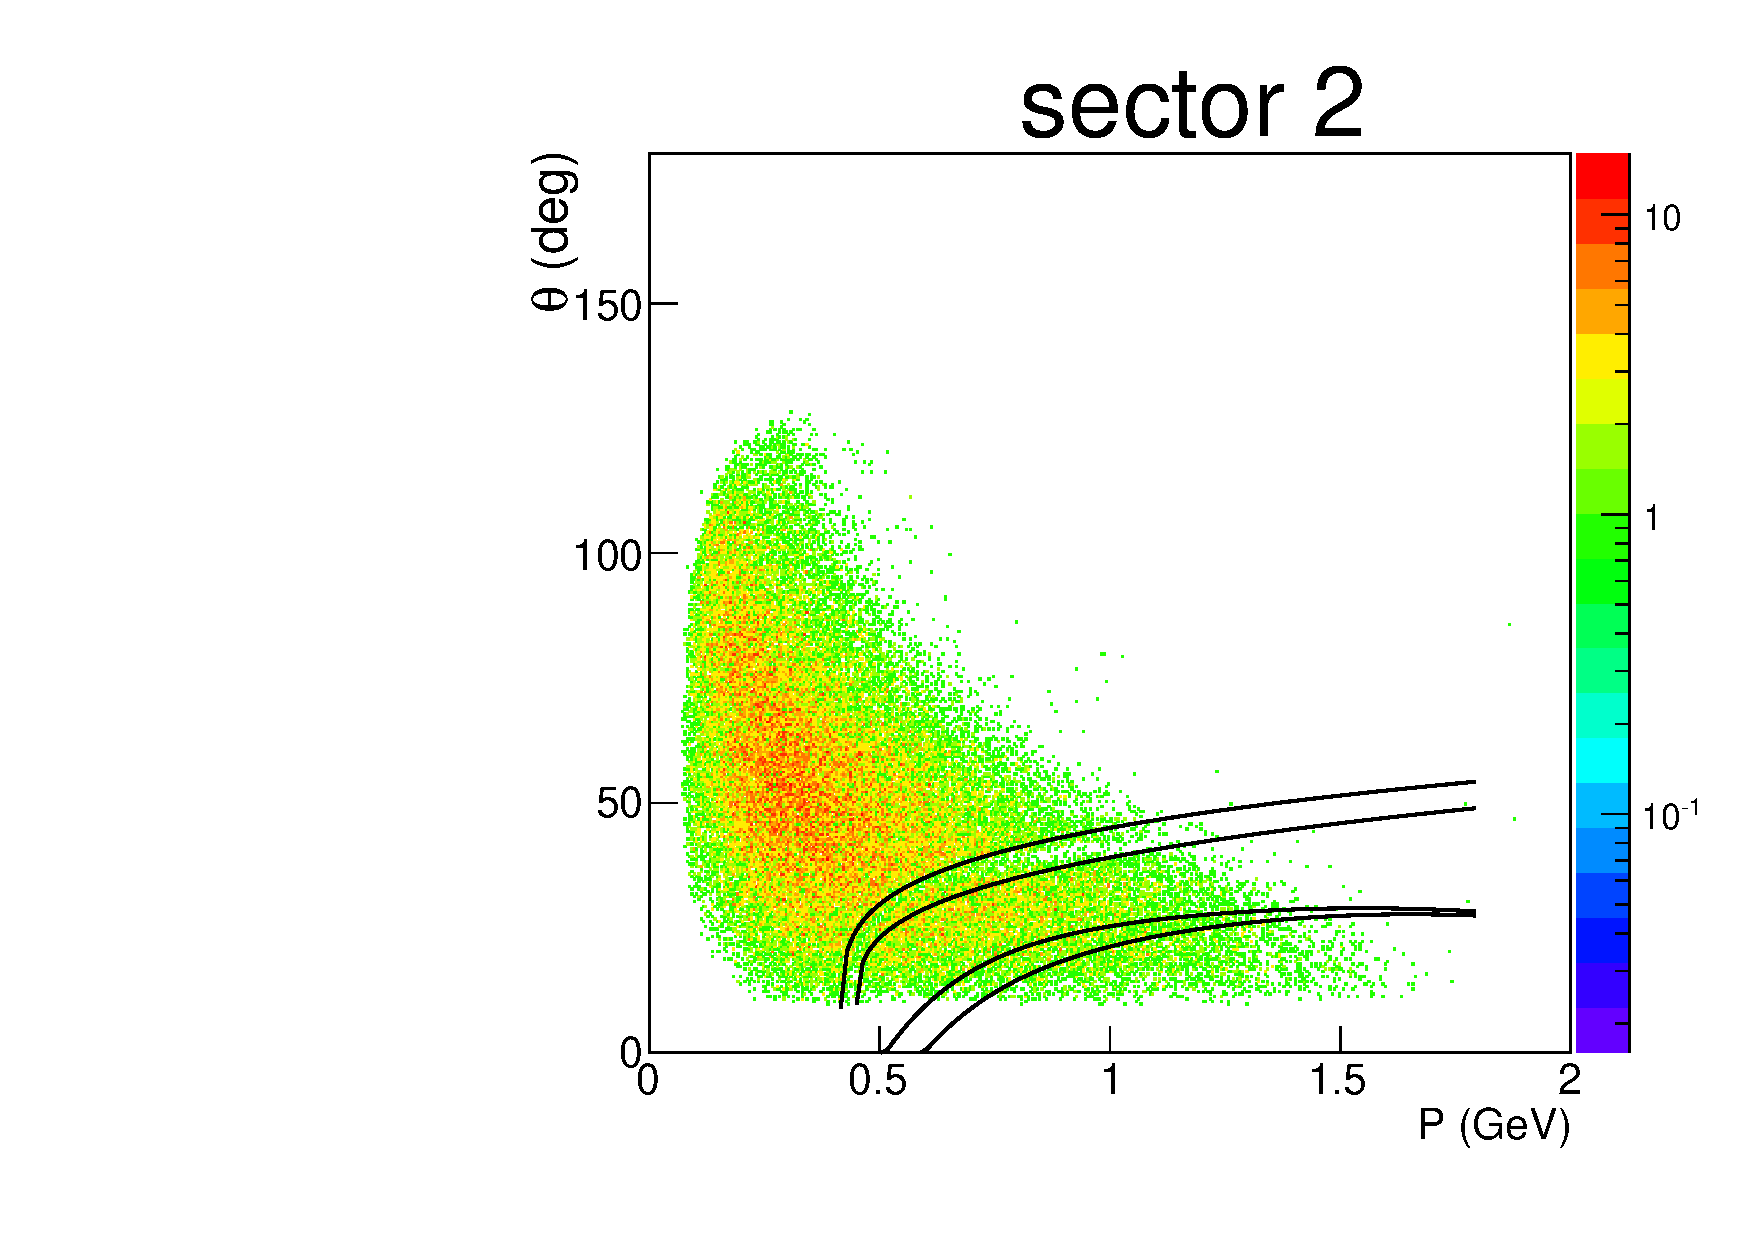
\includegraphics[width=5cm]{pictures/other_cuts/fiduch/th_vs_p_pip_sim/pip_th_vs_p_sim_sector2.pdf}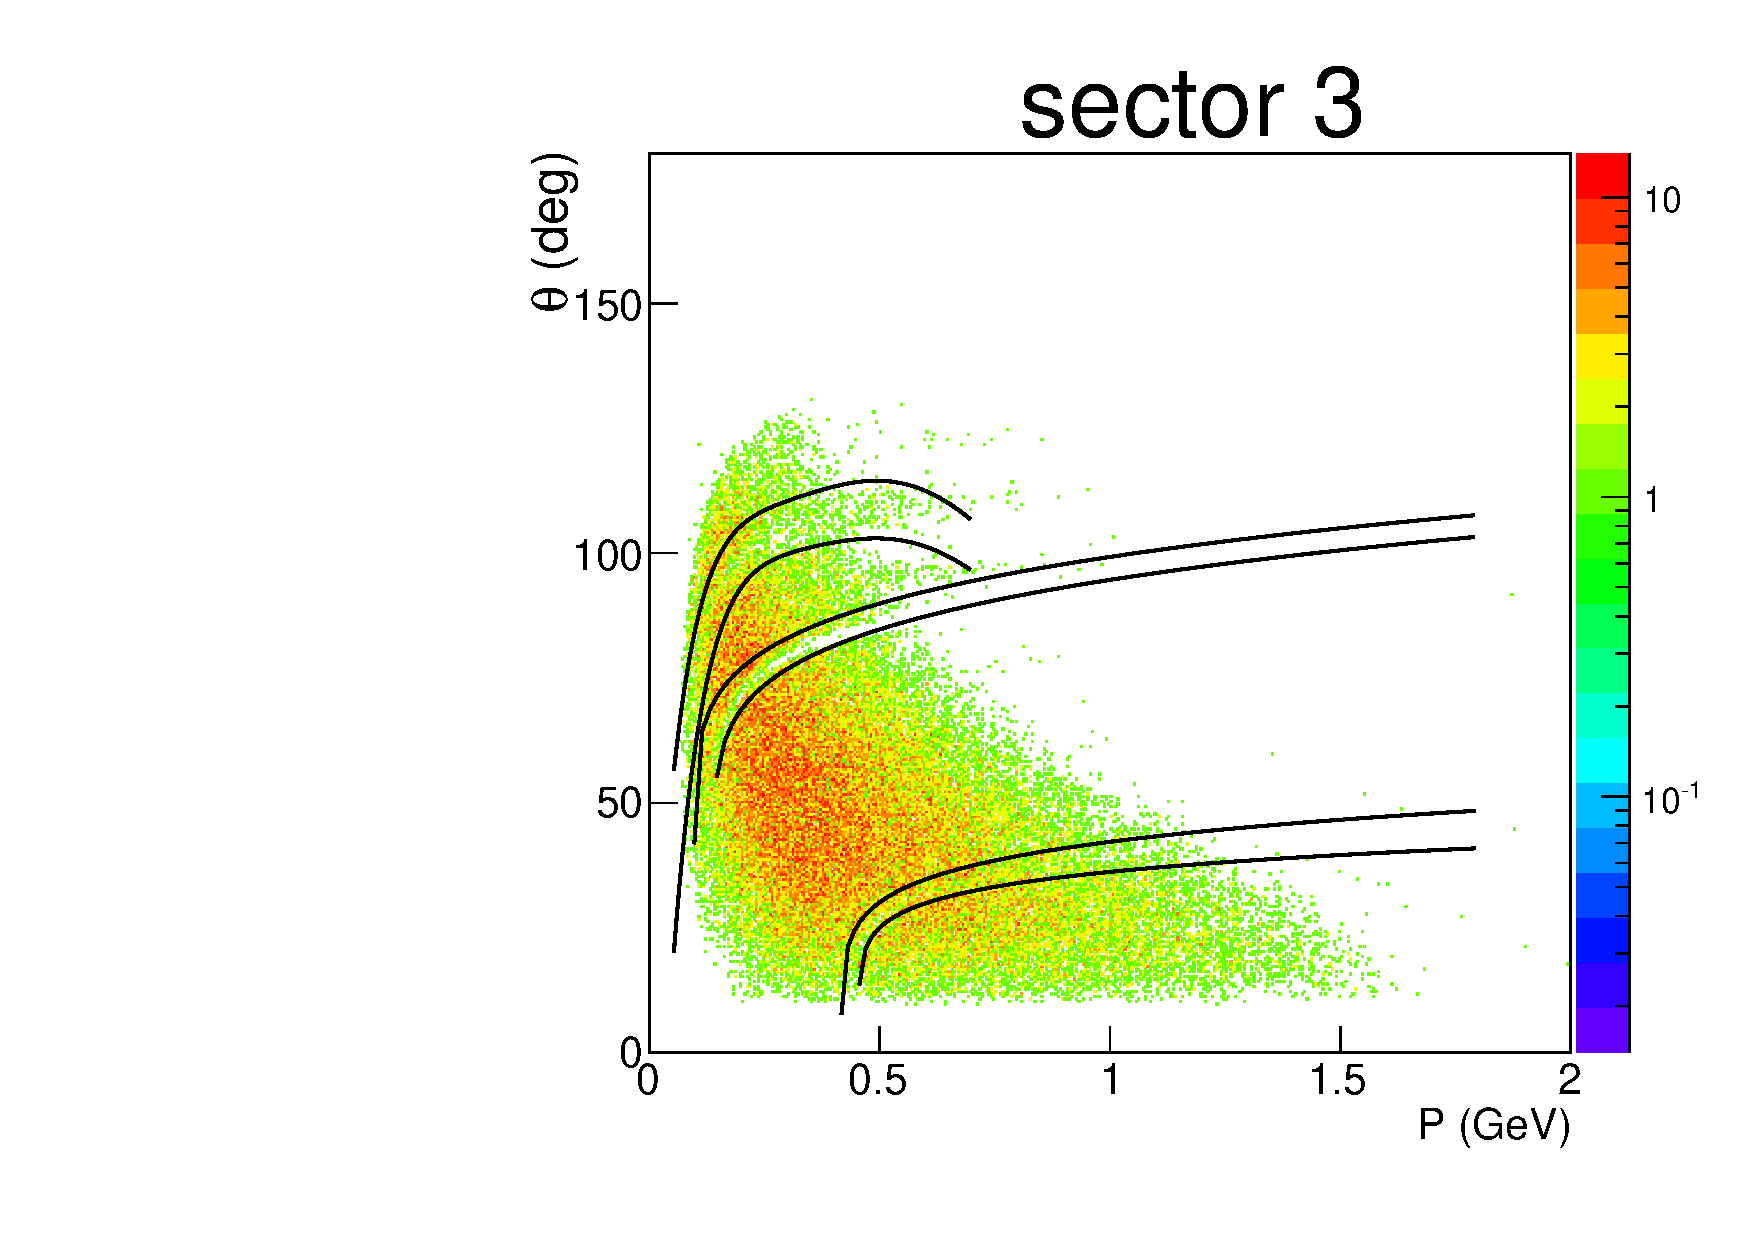
\includegraphics[width=5cm]{pictures/other_cuts/fiduch/th_vs_p_pip_sim/pip_th_vs_p_sim_sector3.pdf}
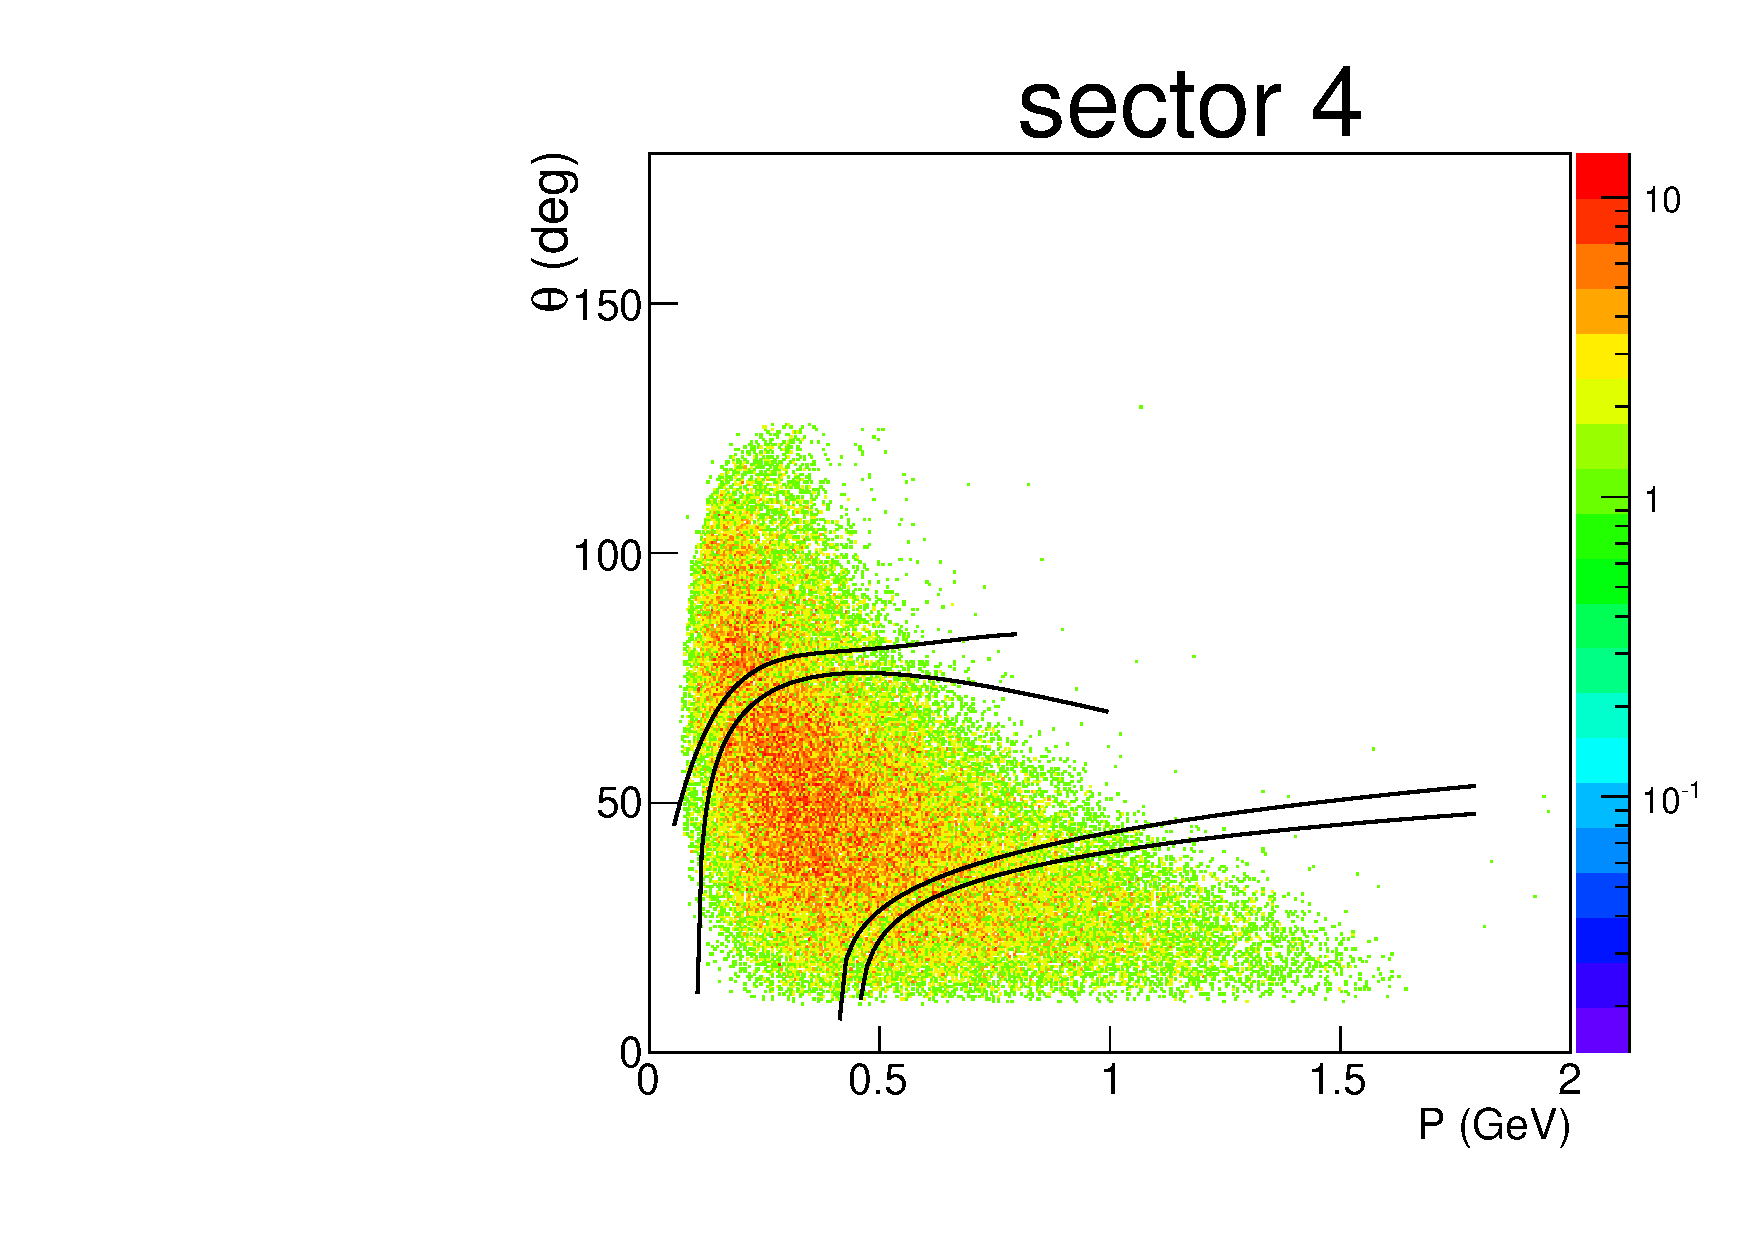
\includegraphics[width=5cm]{pictures/other_cuts/fiduch/th_vs_p_pip_sim/pip_th_vs_p_sim_sector4.pdf}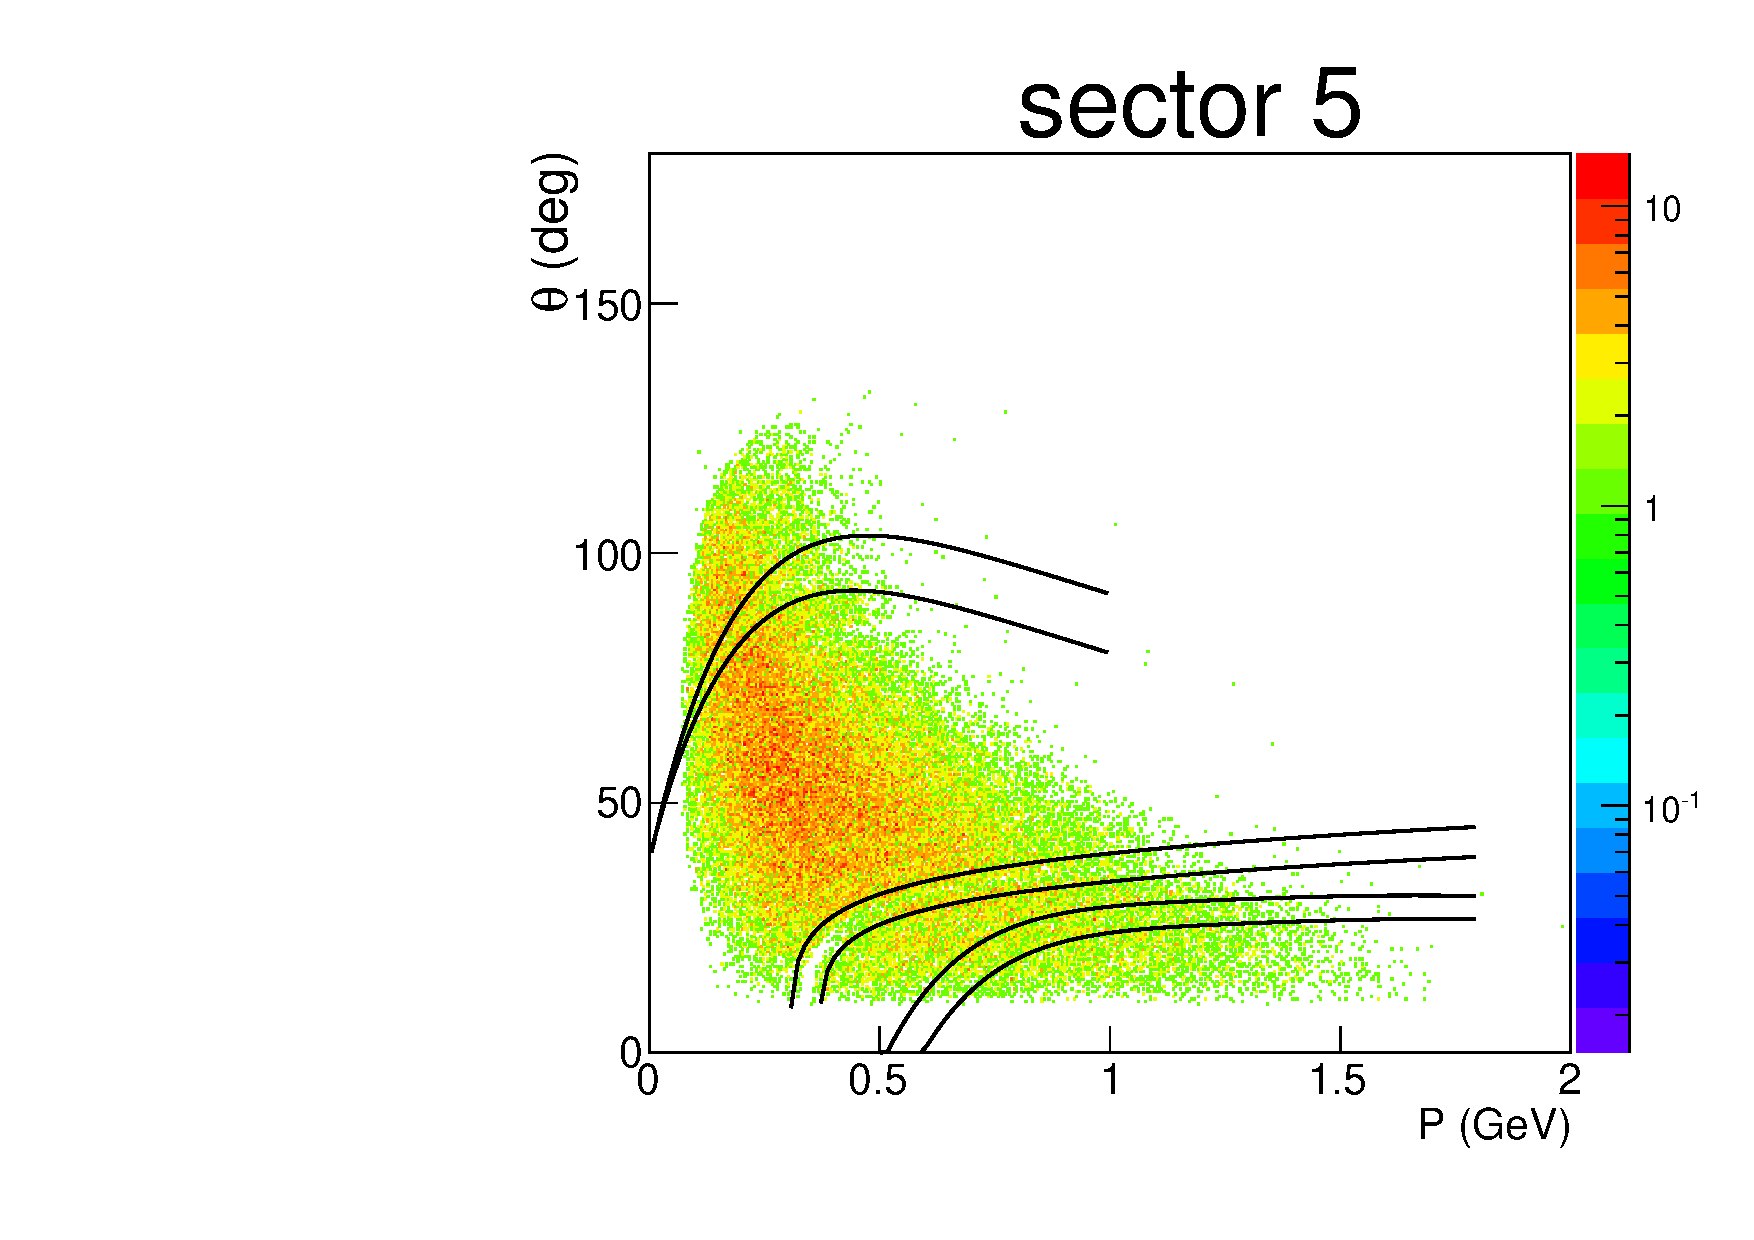
\includegraphics[width=5cm]{pictures/other_cuts/fiduch/th_vs_p_pip_sim/pip_th_vs_p_sim_sector5.pdf}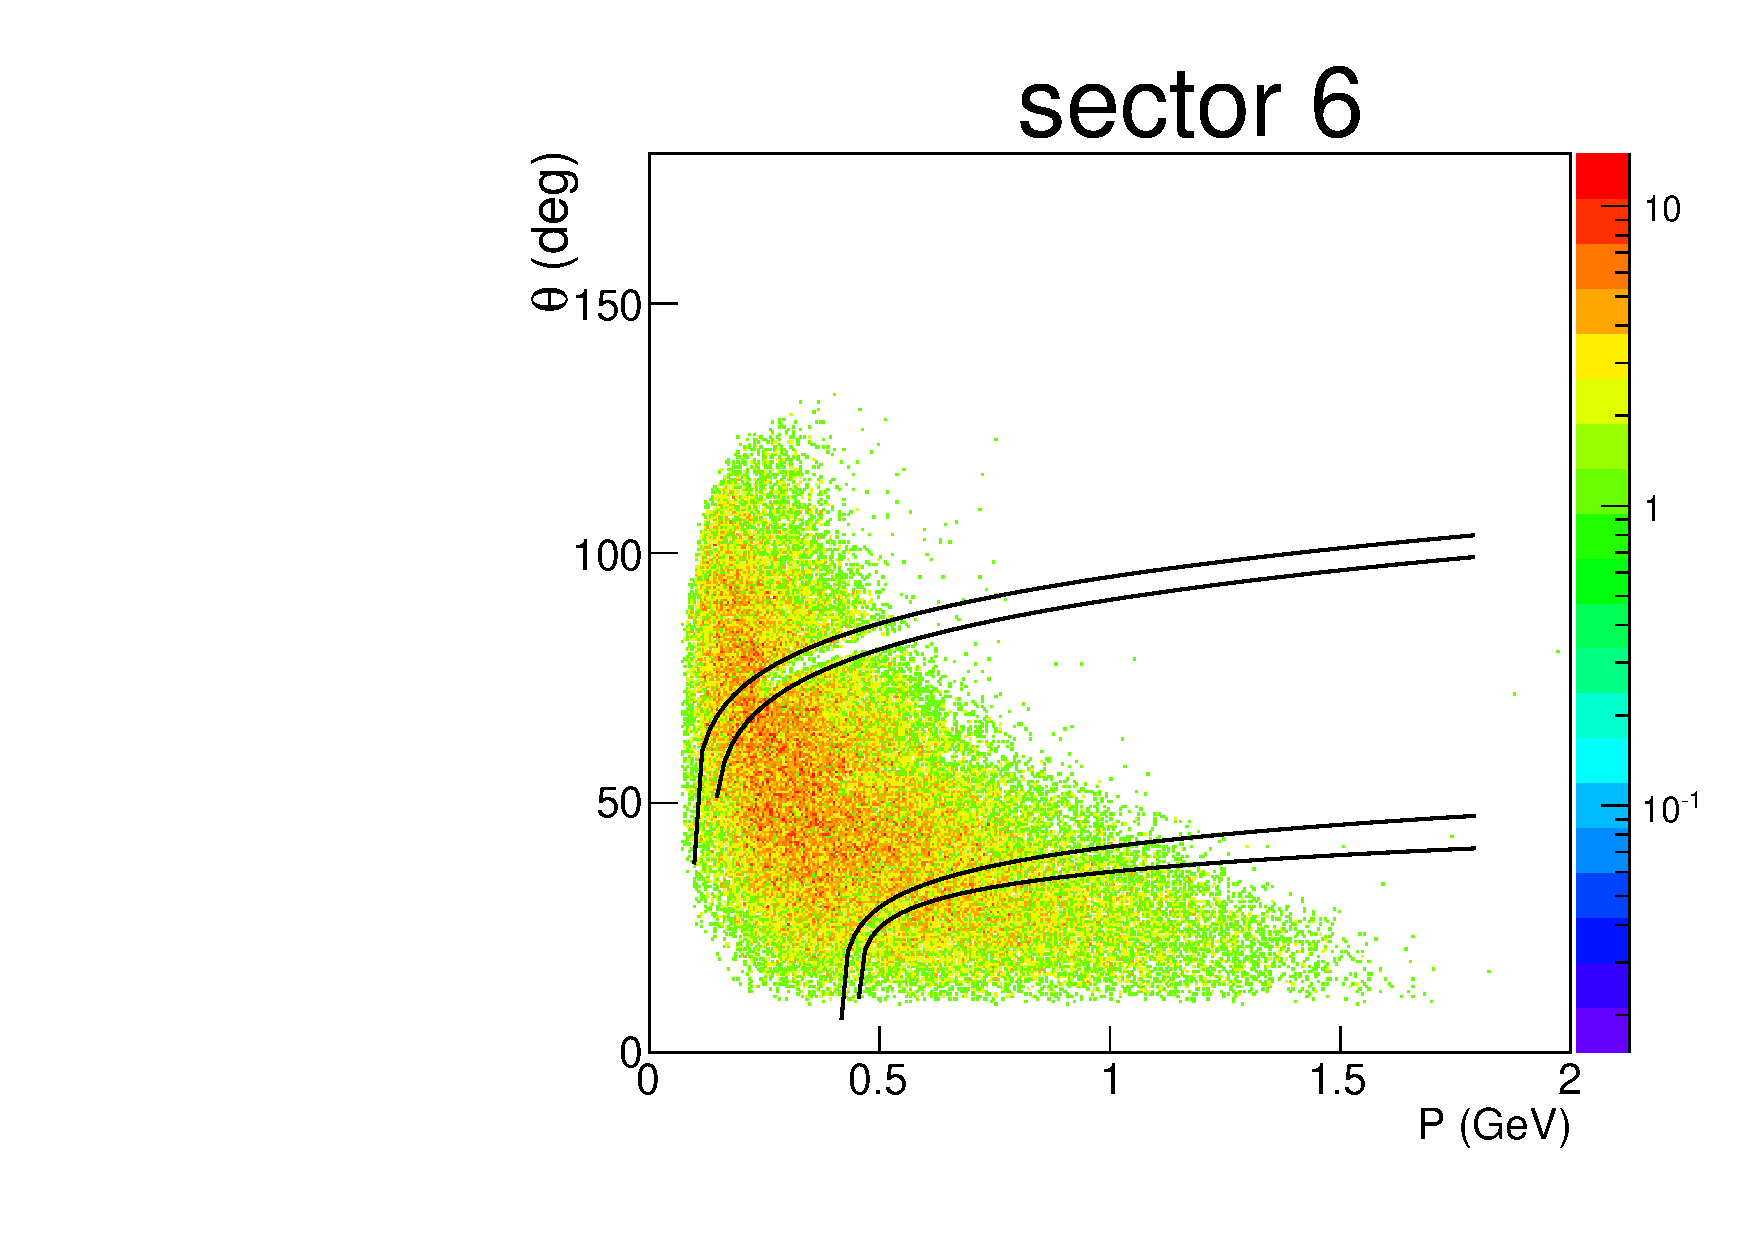
\includegraphics[width=5cm]{pictures/other_cuts/fiduch/th_vs_p_pip_sim/pip_th_vs_p_sim_sector6.pdf}
\end{framed}
\end{minipage}
%\end{framed}
\caption{\small $\theta$ versus momentum distributions for real $\pi^{+}$ events (upper frame)  and for Monte Carlo events (lower frame) for all six CLAS sectors. Black curves show cuts applied to remove inefficient areas. \label{fig:other_cuts_positive_th_vs_p_piplus}}
\end{center}
\end{figure}


%\begin{figure}[htp]
%\begin{center}
%\begin{framed}
%\includegraphics[width=5cm]{pictures/other_cuts/fiduch/th_vs_p_pip/pip_th_vs_p_sector1.pdf}
%\includegraphics[width=5cm]{pictures/other_cuts/fiduch/th_vs_p_pip/pip_th_vs_p_sector2.pdf}
%\includegraphics[width=5cm]{pictures/other_cuts/fiduch/th_vs_p_pip/pip_th_vs_p_sector3.pdf}
%\includegraphics[width=5cm]{pictures/other_cuts/fiduch/th_vs_p_pip/pip_th_vs_p_sector4.pdf}
%\includegraphics[width=5cm]{pictures/other_cuts/fiduch/th_vs_p_pip/pip_th_vs_p_sector5.pdf}
%\includegraphics[width=5cm]{pictures/other_cuts/fiduch/th_vs_p_pip/pip_th_vs_p_sector6.pdf}
%\end{framed}
%\caption{\small $\theta$ versus momentum distributions for $\pi^{+}$ . \label{fig:eother_cuts_pip_th_vs_p}}
%\end{center}
%\end{figure}








\section{Data quality check}
\label{qcheck}

During the quite long experimental run the variations of the experimental conditions, like the target density deviation or improper operation of some parts of the detector, can lead to different yields of events. Only parts of the run with relatively stable event rates are selected for the analysis.
For that purpose cuts on DAQ live time and number of events per Faraday cup (FC) charge are used. 

FC charge updates with given frequency, so the whole run time can be divided into so-called {\em blocks}. Each {\em block} corresponds to the portion of time between two FC charge readouts. FC charge readout happens approximately once in ten seconds. The {\em block} number ranges from one to the maximum number over the run time. The first and last {\em blocks} in each run file are excluded from the analysis since FC readout is not synchronized with begin/end of the file.

DAQ live time is the portion of time within the {\em block} during which the DAQ is able to accumulate events. A significant deviation of the live time from the average value indicates event rate alteration. For instance, if the live time is close to one, then the event rate is too low and vice versa.
In Fig.~\ref{fig:other_cuts_qcheck2d}  DAQ live time and  yields of elastic and inclusive events normalized to FC charge are shown as function of {\em block} number. {\em Blocks} between the horizontal red lines in Fig.~\ref{fig:other_cuts_qcheck2d} are selected for the analysis.
Due to the enormous amount of {\em blocks} all of them can not be made visible in two dimensional histogram, so y-axis projections of histograms in Fig.~\ref{fig:other_cuts_qcheck2d} are produced (see Fig.~\ref{fig:other_cuts_qcheck1d}). The horizontal red cut lines in Fig.~\ref{fig:other_cuts_qcheck2d} correspond to the vertical red cut lines in Fig.~\ref{fig:other_cuts_qcheck1d}.




\begin{figure}[htp]
\begin{center}
\frame{\includegraphics[width=12cm]{pictures/other_cuts/qcheck/qcheck2d.pdf}}
\caption{\small  In the top plot DAQ live time is shown as function of {\em block} number. Each {\em block} corresponds to  the portion of events that is accumulated during a single Faraday cup charge reading cycle. {\em Block} numbers range from one to the maximum number and represents the run duration in Faraday cup reading units. In the middle plot the number of inclusive events accumulated within each {\em block} divided by FC charge accumulated during the {\em block} is  plotted versus {\em block} number. Bottom plot shows the number of elastic events accumulated within each {\em block} divided by FC charge accumulated during the {\em block} as function of {\em block} number. Horizontal red lines show the applied cuts.   \label{fig:other_cuts_qcheck2d}}
\end{center}
\end{figure}

\begin{figure}[htp]
\begin{center}
\frame{\includegraphics[width=12cm]{pictures/other_cuts/qcheck/qcheck1d.pdf}}
\caption{\small Number of {\em block} occurrences (see explanation in the text) as function of DAQ live time (left plot), inclusive event yield normalized to FC charge  (middle plot), and  elastic event yield normalized to FC charge (right plot). \label{fig:other_cuts_qcheck1d}}
\end{center}
\end{figure}


\section{Vertex cut}
\label{vertex_cut}

The target is specific to the e1e experiment and its setup is presented in Fig.~\ref{fig:vertex_cut_e1etarget}. It has a conical shape with diameter varying from 0.4 to 0.6 cm. In some instances cooling system could not extract all the heat generated by the beam and the hydrogen in the target cell could boil. If bubbles stay along the beamline, the real luminosity would be different from the expected value and the absolute measurement will lack accuracy. The conical shape helps to direct bubbles upwards and into a wider area of the target, thus clearing the beamline. The forward aluminum window is made exactly the same as the entry/exit windows of the target cell and can serve for both  the estimation of the number of events originated in the target windows and to precisely measure target $z$ position in the beamline.

In Fig.~\ref{fig:vertex_cut_empty} distributions of electron coordinate $z$ at the interaction vertex are shown for events from both empty and full target runs for six CLAS sectors. The vertex coordinate $z$ is taken from DCPB bank, where already beam-offset corrected values are stored. However small vertex corrections are made to shift the peak that corresponds to the forward aluminum window to the same position for full and empty target runs. Vertical green lines in Fig.~\ref{fig:vertex_cut_empty} show the cut that is applied in addition to the empty target event subtraction. 

In Fig.~\ref{fig:vertex_cut_sim} event distributions after subtraction of empty target contribution are shown in comparison with Monte Carlo events both reconstructed and generated. As it can be seen in Fig.~\ref{fig:vertex_cut_sim} the simulation reproduces data well enough.

 To reduce the number of events  in which the electron comes from one and any hadron from another event, additional cuts on the difference of $z$ coordinates of particles at the vertex are applied. These cuts do not allow the registered particles to have $z$ vertices farther apart than 4 cm. 

\begin{figure}[htp]
\begin{center}
\frame{\includegraphics[width=9cm]{pictures/other_cuts/vertex/e1e_target.pdf}}
\caption{\small The target cell and support structure used during e1e run period. \label{fig:vertex_cut_e1etarget}}
\end{center}
\end{figure}

\begin{figure}[htp]
\begin{center}
\frame{\includegraphics[width=11cm]{pictures/other_cuts/vertex/vertex_empty.pdf}}
\caption{\small Distributions of the electron $z$ coordinate at the vertex for full (blue curves) and empty (red curves) target runs for six CLAS sectors. Vertical green lines show the applied cuts. Both full and empty target distributions are normalized to the corresponding FC charge. \label{fig:vertex_cut_empty}}
\end{center}
\end{figure}

\begin{figure}[htp]
\begin{center}
\frame{\includegraphics[width=11cm]{pictures/other_cuts/vertex/vertex_sim.pdf}}
\caption{\small Distributions of the electron $z$ coordinate at the vertex for data (blue curves) and Monte Carlo (green curves - reconstructed, red - generated)  events for six CLAS sectors. For data empty target contributions are subtracted. All distributions are normalized to the maximum. \label{fig:vertex_cut_sim}}
\end{center}
\end{figure}




\section{Exclusivity cut}
\label{excl_cut}

Due to the experimental conditions the statistics of the double-pion events with all final hadrons registered is rather limited. Moreover, registration of all final hadrons leads to a limited acceptance, so the missing mass technique, when one of the final hadrons is  not registered, is the best choice for the double-pion cross section extraction.


For the analyzed reaction one can distinguish four topologies:
\begin{itemize}
\item $e p \rightarrow e' p' \pi^{+} X$
\item $e p \rightarrow e' p' \pi^{-} X$
\item $e p \rightarrow e' \pi^{+} \pi^{-} X$
\item $e p \rightarrow e' p \pi^{+} \pi^{-} X$
\end{itemize} 

These topologies are defined in a way they do not overlap. For example the topology $e p \rightarrow e' p' \pi^{+} X$ requires the presence of $e'$, $p'$ and $\pi^{+}$ candidates and absence of $\pi^{-}$ candidates, avoiding in this way double counting.


For the case when one of the final hadrons is not registered, the missing mass $M_{X}$ for the reaction $e p \rightarrow e' h_1 h_2 X$ is determined by 



\begin{equation}
M_{X}^{2} = (P_{e} + P_{p} -P_{e'} - P_{h_1} - P_{h_2})^{2},
\label{eg:miss_mass}
\end{equation} 
where $P_{h_1}$ and $P_{h_2}$ are the four-momenta of the registered final hadrons, $P_{e}$ and $P_{p}$ - four-momenta of initial electron and proton, and $P_{e'}$ - four-momentum of the scattered electron.

While for the events with all final hadrons registered, the missing mass $M_{X}$ for the reaction $e p \rightarrow e' p' \pi^+ \pi^- X$ is given by

\begin{equation}
M_{X}^{2} = (P_{e} + P_{p} -P_{e'} - P_{\pi^+} - P_{\pi^-} - P_{p'})^{2},
\label{eg:miss_mass_zero}
\end{equation} 
where $P_{e}$, $P_{p}$, $P_{e'}$, $P_{\pi^+}$, $P_{\pi^-}$,  and $P_{p'}$  are the four-momenta of the initial and final particles.

Distributions of the missing mass squared for various topologies are shown in Fig.~\ref{fig:excl_miss_mass} for different $W$ bins in comparison with Monte Carlo. The top row in Fig.~\ref{fig:excl_miss_mass} stands for the $\pi^-$-missing topology, the second row - for $\pi^+$-missing topology, the third row - for proton-missing topology, and the bottom row for the case when all final hadrons are registered. The green arrows show the applied cuts. The $\pi^-$-missing topology contributes the biggest part to the statistics (about 70\%), while events from other topologies populate kinematical areas with no acceptance for the $\pi^-$-missing topology. 
By combining events from various topologies one can reduce contributions from kinematical cells with zero acceptance (so-called empty cells) (see Sect.~\ref{zero_acc}).

The simulation is carried out with the JM05 version of double-pion production model \cite{Ripani:2000va,Aznauryan:2005tp,Mokeev:2005re} and includes inclusive radiative effects according to \cite{Mo:1968cg}. More details about Monte Carlo simulation are in Sect.~\ref{eff_aval}.



The contribution from the other exclusive channels (exclusive background) to the events within the exclusivity cuts is also taken into account by the Monte Carlo simulation. Most of the exclusive background events come from the $e p \rightarrow e' p' \pi^{+} \pi^{-} \pi^{0}$ channel. Both double-pion and three-pion channels are generated together with the relative weight of their cross sections taken from~\cite{Wu:2005wf}.  A phase space distribution is assumed for the $3\pi$ events. The $3\pi$ background can be barely seen as a separate peak on the right side of the missing mass squared distributions for the exclusive topology in last two $W$ bins (see Fig.~\ref{fig:excl_miss_mass} bottom row). For the other topologies the $3\pi$ background can not be seen as a separate peak and it manifests itself as a contribution to the tail on the right side of the missing mass squared distributions.

\begin{figure}[htp]
\begin{center}
\frame{\includegraphics[width=0.95\textwidth]{pictures/other_cuts/miss_mass/miss_mass.pdf}}
\caption{\small Missing mass squared distributions for various bins in $W$ for $Q^2$ from 0.45~GeV$^2$ to 0.5~GeV$^2$. Blue curves show real and red curves Monte Carlo events. The top row corresponds to $\pi^-$-missing topology, the second to $\pi^+$-missing topology, the third to proton-missing topology, and the bottom to the fully exclusive topology. Green arrows show the applied exclusivity cuts.  \label{fig:excl_miss_mass}}
\end{center}
\end{figure}

\section{Missing energy cut}
\label{miss_energ}

To clean up event samples from misidentified and out-of-time particles, a cut on the missing energy is used in addition to the missing mass cut (Sect.~\ref{excl_cut}). It limits the missing energy to be greater than $m_{miss\_hadron} - 50$~MeV, where $m_{miss\_hadron}$ is equal to the mass of the missing hadron ($\pi^-$, $\pi^+$, or proton depending on the topology) or zero for the topology where all final hadrons are registered. The position of this cut is shown by the green vertical lines in Fig.~\ref{fig:miss_en}.
%\section{Invariant mass cut}
%\label{inv_mass}
\begin{figure}[htp]
\begin{center}
\frame{\includegraphics[width=0.95\textwidth]{pictures/other_cuts/miss_en/miss_en.pdf}}
\caption{\small   Missing energy distributions for various topologies. Left plot corresponds to the topology where all final hadrons are registered and other plots correspond to the topologies with missing $\pi^-$, $\pi^+$, or proton, respectively. Green vertecal lines show the applied cut. All events on the right side of the lines are selected as good for analysis.\label{fig:miss_en}}
\end{center}
\end{figure}

\section{Binning and kinematical coverage}
\label{cuts_sum}

After all described above cuts and corrections about 2.5 million double-pion events survive and are used for the cross section calculation. Figure \ref{fig:summary_q2vsw} shows the available kinematical coverage in electron variables. double-pion cross sections are calculated in 2D cells within the white boundaries in Fig.~\ref{fig:summary_q2vsw}.

\begin{figure}[htp]
\begin{center}
\frame{\includegraphics[width=12cm]{pictures/other_cuts/summary/q2vsw/q2vsw.pdf}}
\caption{\small $Q^2$ versus $W$ distribution populated with selected double-pion events. The cross section is calculated in 2D cells within the white boundaries.  \label{fig:summary_q2vsw}}
\end{center}
\end{figure}

The binning in the final hadron variables is chosen according to the statistics left after the event selection (see Tab.~\ref{tab:summary_bins}) and takes into account the fact that the cross section is small in the $W$ area near the double-pion production threshold. A more detailed description of the final hadron variable choice is given in Sect.~\ref{kin_var}.

It also needs to be mentioned that the right boundary of the invariant mass distributions depends on the value of $W$, while the left does not (see Eq.~\ref{eq:inv_mass_boundary}). 
\begin{equation}
\begin{aligned}
M_{left} = m_{h_1} + m_{h_2} \\
M_{right} = W - m_{h_3}, \label{eq:inv_mass_boundary}
\end{aligned}  
\end{equation}
where $M_{left}$ and $M_{right}$ are the left and right boundaries of  the invariant mass distribution. $m_{h_1}$, $m_{h_2}$, and $m_{h_3}$ are the masses of final hadrons. The value of $W$ is taken in the center of the corresponding $W$ bin.

It leads to the fact that invariant mass distributions are broader at high $W$ and hence a more detailed binning in that area is necessary (see Tab.~\ref{tab:summary_bins}).

%To take into account the finite detector resolution and the fact that the right boundary of the invariant mass distribution is calculated using the $W$ value at the center of the bin, the left and right boundaries of invariant mass distributions are widened with respect to their theoretical values (Eq.~\ref{eq:inv_mass_boundary}) by 50~MeV to the left and right sides, respectively.

Since $M_{right}$  is calculated using the value of $W$ in the center of the corresponding $W$ bin some events are located beyond the boundaries determined by Eq.~\ref{eq:inv_mass_boundary}. Therefore the binning in invariant mass needs special attention.
Firstly the bin width is determined as:
\begin{equation}
\begin{aligned}
width = \frac{M_{right}-M_{left}}{N_{bins}-1}, \label{eq:bin_width}
\end{aligned}  
\end{equation} 
where $N_{bins}$ is the number of bins. 

Then the invariant mass distributions are obtained with the number of bins $N_{bins}$ and the left boundary of the first bin is set to $M_{left}$. That makes the last bin to be situated completely out of the boundaries given by Eq.~\ref{eq:inv_mass_boundary}. Although the cross section obtained in this bin is very small, it is kept in analysis since its content contributes to all other cross sections obtained by integration over the corresponding invariant mass. 
After the binning corrections this effect is assumed to be taken into account and this last bin in invariant masses is neglected. 

It needs to be mentioned that the next to last bin in each invariant mass also needs special attention. Since the cross sections are obtained in $W$ bin, the right boundaries of the invariant mass distributions vary for different events within this bin. In Fig.~\ref{fig:mass_corr} the distribution of the invariant mass of the two final hadrons $X_{1}$ and $X_{2}$ is schematically illustrated for the bin in $W$ from $W_{left}$ to $W_{right}$. 
The green and red vertical dashed lines show  maximal invariant mass values that can be reached with $W_{left}$ and $W_{right}$, respectively, while the vertical black dashed lines show the boundaries of the next to last bin in the invariant mass.
As it is seen in Fig.~\ref{fig:mass_corr} events in this bin with $W$ between $W_{left}$ and $M_{right}^{N_{bins}-1} = W_{center} - m_{X_{3}}$ are distributed in the range in $M_{X_{1}X_{2}}$, which is less than invariant mass bin width defined by Eq.~\ref{eq:bin_width}.

Correction for this effect is made using the new double pion event generator~\cite{Skorodum:EG}. For that purpose for each invariant mass two  one-dimensional distributions are generated in each $W$ bin. The first one mimics the data distribution, for which all events in the next to last bin are divided by the same bin width defined by Eq.~\ref{eq:bin_width}.  For the second one events with $W$ between $W_{center}$ and $W_{right}$ are divided by the same bin width defined by Eq.~\ref{eq:bin_width}, while events with $W$ between $W_{left}$ and $W_{center}$ are divided by the bin width that is individual for each event and equal to $W - m_{X_{3}} - M_{left}^{N_{bins}-1}$. The correction factor, by which obtained single-differential cross sections in the next to last bin should be multiplied, is defined as the ratio of the second distribution over the first one. This factor typically varies from 5\% to 10\%. 


\begin{figure}[htp]
\begin{center}
\frame{\includegraphics[width=12cm]{pictures/cross_sction/mass_corr/mass_tex.pdf}}
\caption{\small Schematic representation of the cross sections in the next to last bin in the invariant mass $(M_{X_{1}X_{2}})$ for various $W$. Green and red vertical dashed lines show  maximal invariant mass values that can be reached with $W_{left}$ and $W_{right}$, respectively, while vertical black dashed lines show the boundaries of the next to last bin in the invariant mass.  \label{fig:mass_corr}}
\end{center}
\end{figure}



\begin{table}[htp]
\centering 

\begin{tabular}{|c|C{0.13\textwidth}|C{0.13\textwidth}|C{0.15\textwidth}|C{0.18\textwidth}|}
\hline \multirow{2}{*}{\diagbox[width=3cm, height=2.3cm]{\raisebox{7pt}{$W$ range}}{\raisebox{-10pt}{Variable}}} &Number of bins in invariant mass $M$ &Number of  bins in polar angle $\theta$ &Number of bins in  azimuthal angle $\varphi$ &Number of bins in angle between two planes $\alpha$ \\
\hline
 1.3 - 1.35 GeV & 8 & 6 & 5 & 5\\
\hline
1.35 - 1.4 GeV & 10 & 8 & 5 & 6\\
\hline 
 1.4 - 1.45 GeV & 12 & 10 & 5 & 8\\
\hline 
 $ > 1.45$ GeV & 12 & 10 & 8 & 8\\
\hline 
\end{tabular}
\caption{\small Number of bins for the given final hadron variables. \label{tab:summary_bins}}
\end{table}
